\documentclass[a4paper]{report}

% \usepackage[utf8]{inputenc}
% \usepackage[T1]{fontenc}
% \usepackage{textcomp}
\usepackage[english]{babel}
\usepackage{amsmath, amssymb}
\usepackage[separate-uncertainty=true, multi-part-units=single, per-mode=power]{siunitx}
\usepackage[]{subfig}
\usepackage[colorlinks=true, anchorcolor=blue, linkcolor=blue, citecolor=blue, bookmarks=false,hyperfootnotes=false]{hyperref}
\usepackage[margin=1in]{geometry}
\usepackage{color,soul}
\usepackage{tabularx}
% \usepackage[clean]{svg}


% figure support
\usepackage{import}
\usepackage{xifthen}
\pdfminorversion=7
\usepackage{pdfpages}
\usepackage{transparent}
\usepackage{physics}
\graphicspath{ {./figures/} }
% \setlength{\parindent}{0pt}
\usepackage{chngcntr}
\usepackage{verbatim}
\usepackage{indentfirst}
\numberwithin{equation}{section}
\counterwithin{figure}{section}
\newcommand{\incfig}[1]{%
		\def\svgwidth{\columnwidth}
		\import{./figures/}{#1.pdf_tex}

}

\pdfsuppresswarningpagegroup=1

% for citations / references
\usepackage[style=ieee, url=false]{biblatex}
\addbibresource{lasers_report.bib}

\begin{document}

%----------------------------------------------------------------------------------------
%	TITLE PAGE
%----------------------------------------------------------------------------------------
\begin{titlepage} % Suppresses displaying the page number on the title page and the subsequent page counts as page 1
	\newcommand{\HRule}{\rule{\linewidth}{0.5mm}} % Defines a new command for horizontal lines, change thickness here
	
	\center % Centre everything on the page
	%------------------------------------------------
	%	Headings
	%------------------------------------------------
	
	\textsc{\LARGE Rheinische Friedrich-Wilhelms-Universit\"at Bonn }\\[4cm] % Main heading such as the name of your university/college
	
	\textsc{\Large Advanced Laboratory Course}\\[0.5cm] % Major heading such as course name
	
	\textsc{\large Performed on: April 4th - 5th, 2022}\\[0.5cm] % Minor heading such as course title

	\textsc{\large Submitted on: May 3, 2022}\\[0.5cm] % Minor heading such as course title
	
	%------------------------------------------------
	%	Title
	%------------------------------------------------
	
	\HRule\\[0.4cm]
	
	{\huge\bfseries A249: Laser Gyroscope}\\[0.4cm] % Title of your document
	
	\HRule\\[1.5cm]
	
	%------------------------------------------------
	%	Author(s)
	%------------------------------------------------
	
	\begin{minipage}{0.4\textwidth}
		\begin{flushleft}
			\large
			\textit{Authors}\\
			Keito Watanabe \\
			Paarth Thakkar
		\end{flushleft}
	\end{minipage}
	~
	\begin{minipage}{0.4\textwidth}
		\begin{flushright}
			\large
			\textit{Tutor(s)}\\
			Thorsten Groh \\
			Marc Vöhringer
		\end{flushright}
	\end{minipage}

	\vspace*{5em}

	\begin{minipage}{0.8\textwidth}
		\begin{centering}
			% \large
			\textbf{Abstract}\\[0.2cm]
			 
		\end{centering}
	\end{minipage}
	
	% If you don't want a supervisor, uncomment the two lines below and comment the code above
	%{\large\textit{Author}}\\
	%John \textsc{Smith} % Your name
	
	%------------------------------------------------
	%	Date
	%------------------------------------------------
	
	%\vfill\vfill\vfill % Position the date 3/4 down the remaining page
	% \vfill\vfill
	
	% {\large\today} % Date, change the \today to a set date if you want to be precise
	
	%------------------------------------------------
	%	Logo
	%------------------------------------------------
	
	%\vfill\vfill
	%\includegraphics[width=0.2\textwidth]{placeholder.jpg}\\[1cm] % Include a department/university logo - this will require the graphicx package
	 
	%----------------------------------------------------------------------------------------
	
	% \vfill % Push the date up 1/4 of the remaining page
	
\end{titlepage}



\tableofcontents

\chapter{Introduction}

The rotation of the Earth has been investigated ever since the advent of calenders. 
The first measurements for the rotation of the Earth has been done by observing the apparent
position of a fixed star, allowing the Mayans to obtain measurements with relative uncertainties of around $10^{-5}$ \cite{Groh2021}.

Today, the rotation of the Earth is measured using interferometry, where radio telescopes
all around the world are linked to construct a very-long base-interferometer system (VBLI). Fig. \ref{fig:vlbi_locs}
show the locations of all radio telescopes under the CONT17 campaign, a continuous VLBI session held for two weeks
in 2017 \cite{Behrend2020}. The relative
uncertainties that are obtained reach approximately $10^{-10}$. Today, the rotation of the Earth is 
measured to be approximately $\SI{72.92}{\micro\radian\per\second}$ along its rotation axis \cite{Groh2021}. \par 

\begin{figure*}[h!]
	\centering
	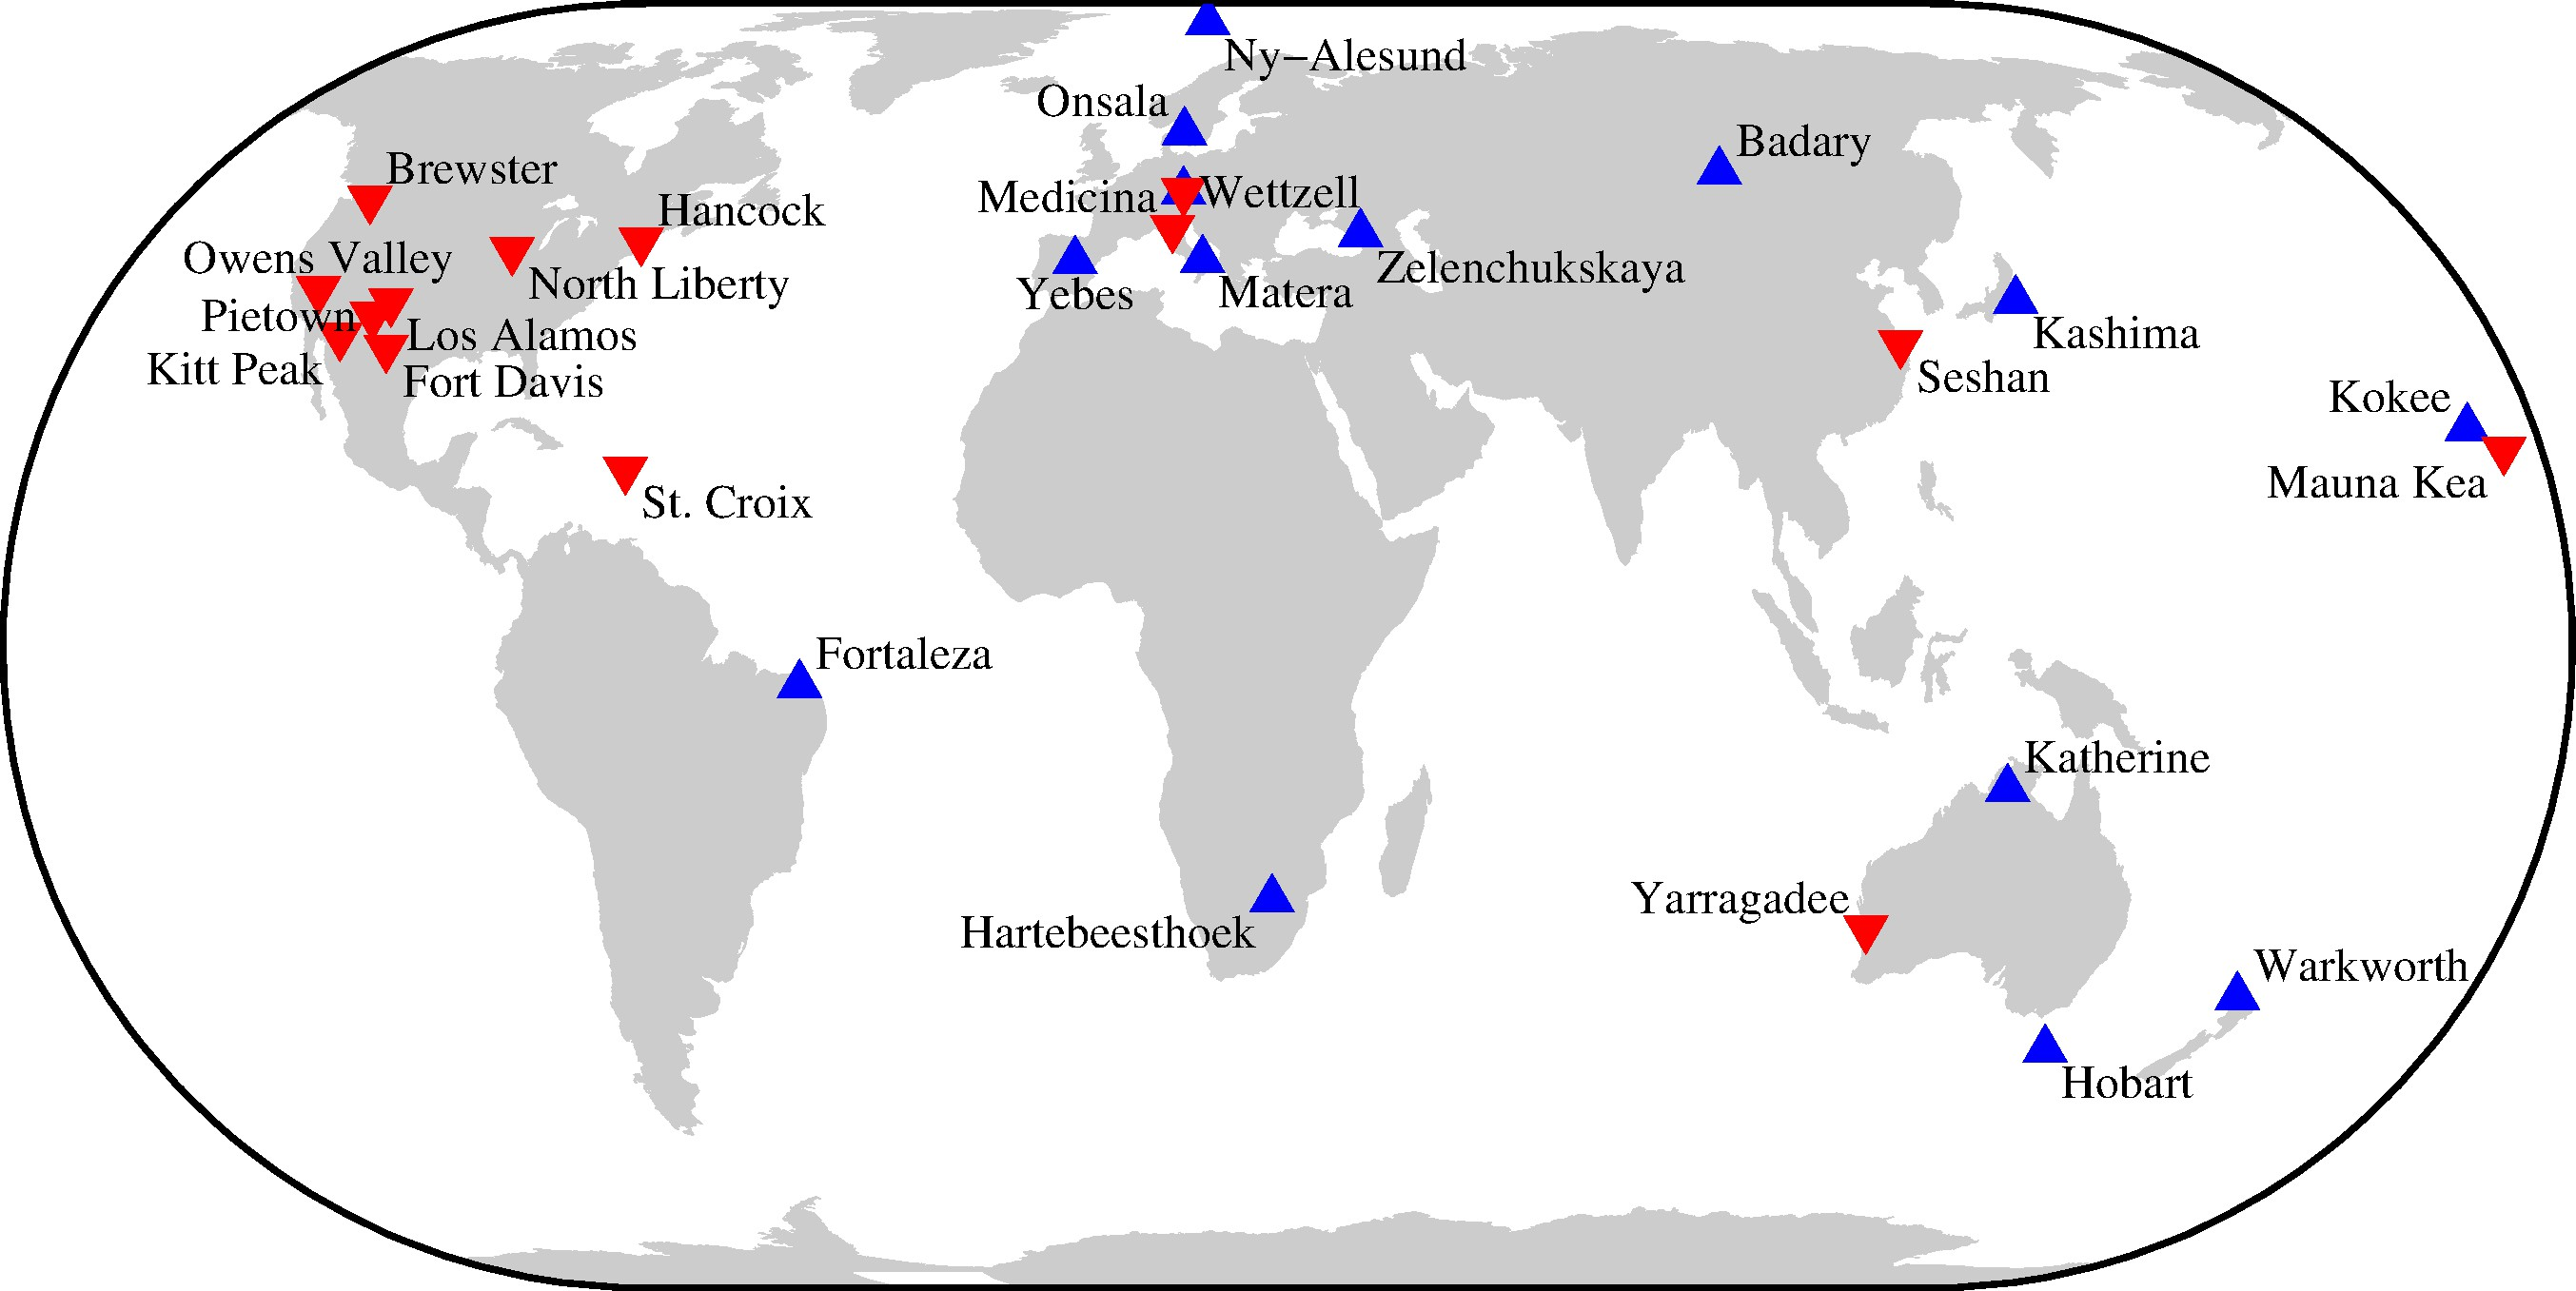
\includegraphics[width=0.6\columnwidth]{cont17_legacy.jpg}
	\caption{Radio telescopes used for CONT17. Both blue and red markers
	indicate legacy stations used for measurements in past sessions.}
	\label{fig:vlbi_locs}
\end{figure*}


Determining the rotation of the Earth allows us to understand the vast phenomena that occur on Earth,
including tidal breaking, seasonal variations, and the Chandler wobble, the nutation that occurs with Earth's
rotation axis. Furthermore, climate change has a strong effect on the rotation rate as the melted ice from the 
polar ice caps gravitate towards the equator, increasing the angular momentum and thus the rotation period of Earth.
This is shown to increase at a rate of $\SI{1.2}{\micro\second}$ per year \cite{Groh2021}. \par 

While the VLBI can determine the rotation rate with high precision, due to the operation times the temporal resolution
is low. As such, transient events such as earthquakes and tides cannot be resolved. As of such, 
laser gyroscopes have been employed to resolve such details. While it lacks in the long-term stability of VLBI,
they have a temporal resolution of approximately an hour or less \cite{Wettzell2005}. The G-ring at the German
Fundamentalstation Wettzell is one of the best ring laser gyroscopes with a sensitivity of around \SI{12}{\pico\radian\per\second\per\sqrt{\hertz}} \cite{Groh2021}. 
See Fig. \ref{fig:gring_gyro} for an image and the setup of the G-Ring gyroscope. Ring laser gyroscopes are still explored today to 
describe other phenomena from the Earth's rotation such as the Lense-Thirring Effect, and gyroscopes such as the GINGERino have been proposed to 
measured such quantities \cite{Beverini2016}.

\begin{figure*}[h!]
	\centering
	\subfloat[]{{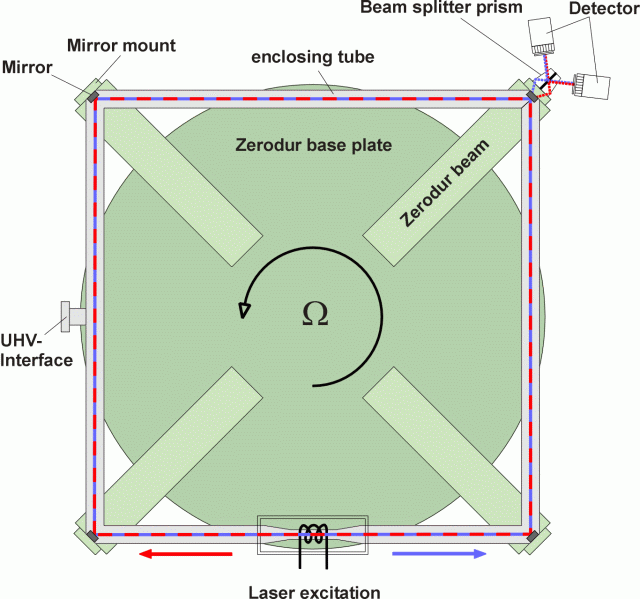
\includegraphics[width=0.4\columnwidth]{gring_gyroscope.png}}}
	\quad
	\centering
	\subfloat[]{{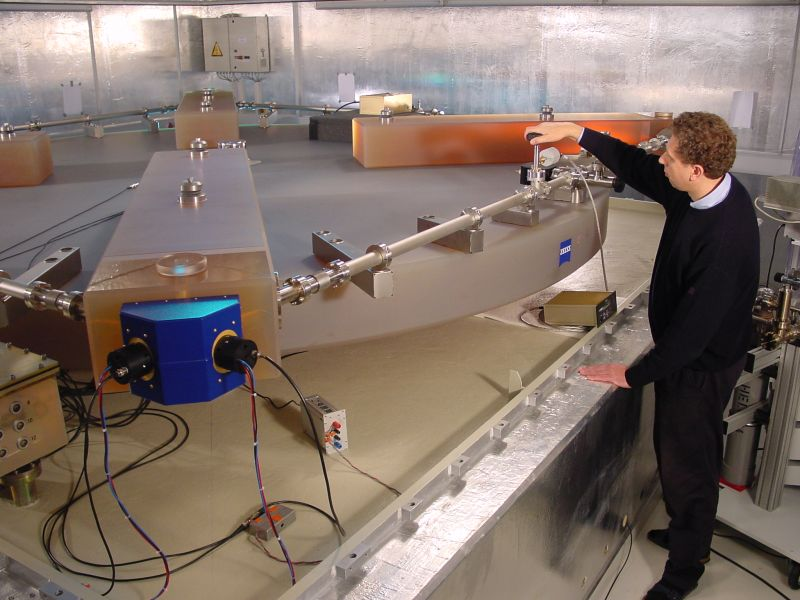
\includegraphics[width=0.4\columnwidth]{G-ring.jpg}}}
	\caption{The G-Ring gyroscope at the Fundamentalstation Wettzell. (a):
	The setup of the gyroscope. (b): Image of the G-ring. Obtained from Ref. \cite{Wettzell2005}.}
	\label{fig:gring_gyro}
\end{figure*}

% The first time that a ring laser gyroscope was employed for measurement of the rotation of the Earth was 
% from the Michelson-Gale experiment, conducted in 1929. In such experiment, Albert A. Michelson sent counter-propagating beams thorough 
% pipelines with a total effective area of around $\SI{0.2}{\kilo\metre\squared}$. He observed that the fringe difference measured
% was well within the expectations of the analytical fringe shift \cite{Groh2021}. 

% add something about the Michelson-Gale experiment here? maybe not needed. otherwise can also add another figure too

In our experiment, we use a ring laser gyroscope to attempt to measure the rotation rate of the Earth. This is done by employing the Sagnac effect,
which allows us to determine the rotation of an inertial system by the path length difference between two light beams. To observe
the quality of the constructed laser gyroscope, we measure optical cavity parameters such as the free spectral range,
PDH locking error signals, lock-in threshold, and the finesse. We further quantify the stability and sensitivity of the gyroscope by 
determining the Allan deviation. \par 

This paper is structured as follows. Chapter 1 motivates the experiment by elaborating on the usage of ring laser gyroscopes
to determine the rotation rate of the Earth. Chapter 2 describes the theory behind the quantities measured in the experiment. Chapter 3
describes the setup used in our experiment and the method used to determine the relevant quantities for each part of our experiment. 
Chapter 4 shows the pre-laboratory tasks that were required before starting the experiment. Chapter 5 shows the results
that we have obtained and discussions related to the results. Finally, we summarize our findings and address possible outlooks for our experiment
in Chapter 6. 

% should we hyperlink the chapters?


\chapter{Theory}

\section{Gyroscopes}

\subsection{The Sagnac Effect}

The Sagnac effect tells us that whilst the motion between two inertial frames cannot be distinguished, two rotating frames can be 
distinguished, allowing one to directly measure the rotation rate of an inertial system \cite{Groh2021}. This effect was first observed by 
George Sagnac in 1913, whom believed that this experiment was a proof that aether exists in an inertial frame  \cite{Darrigol2014}. This, however, was 
disproven by Max von Laue in 1911 where he showed that the Sagnac effect was compatible with special relativity \cite{Laue1911}. 
However, the interpretation of the Sagnac effect due to the general theory of relativity is still investigated today, 
even though it is already well-known in literature \cite{Benedetto2019}. In our analysis, we utilize the Sagnac effect on a gyroscope to 
measure the rotation rate of the Earth.\par

To observe the Sagnac effect, we consider an interferometer setup with light propagating with wavelength $\lambda$ enclosing an area $\vec{A}$
 with perimeter $P$. Placing such a setup onto a rotating platform with frequency $\vec{\Omega}$, we observe that the optical path that
 each light travels changes. For example, if the table rotates counter-clockwise, then the path of the co-rotating light increases, while that of the other light
decreases (see Fig. \ref{fig:Sagnac_effect}). The Sagnac effect then tells us the resulting phase shift between the two lights:
\begin{equation}
	\delta \phi = \frac{8\pi \vec{A} \cdot \vec{\Omega}}{c \lambda} \propto \vec{A} \cdot \vec{\Omega}.
\end{equation} 

\begin{figure*}[h!]
	\centering
	\includegraphics[width=0.6\columnwidth]{Sagnac_effect.jpg}
	\caption{The Sagnac effect. \textit{Left}: Setup without rotation. The beam moving clockwise (blue) and counter-clockwise (orange)
	have the same optical path length. \textit{Right}: Setup with a clockwise rotation $\Omega$. The path length of the 
	clockwise beam is larger than that of the counter-clockwise beam. Obtained from Ref. \cite{Feng2020}.}
	\label{fig:Sagnac_effect}
\end{figure*}

A more detailed derivation using the relativistic law of velocity addition can be found in Ref. \cite{Benedetto2019}. 

\subsection{Ring Laser Gyroscopes}

\subsubsection{Active Ring Laser Gyroscopes}

In order to incorporate the Sagnac effect within our experiment, we utilize ring laser gyroscopes. A laser is placed within an 
enclosed cavity, and emits two counter-propagating beams. Such beams reflect off mirrors and interfere at the end of their 
propagation. When rotating the platform in which such setup is placed, different interference patterns can be observed, and 
transforms the ring cavity system into a cavity resonator. The corresponding beat frequency $\delta \nu$ observed is then the 
Sagnac frequency, which is given as such:

\begin{equation}
	\delta \nu = \frac{4 \vec{A} \cdot \vec{\Omega}}{P \lambda}.
	\label{eq:Sagnac_freq}
\end{equation}

In our experiment, we only consider square ring cavities so that $A = L^2$ and $P = 4L$, where $L$ is the path length of each arm. 
As such, we can simplify Eq. \ref{eq:Sagnac_freq} as such: 
\begin{equation}
	\delta \nu  = \frac{L \Omega}{\lambda} = n \Omega,
	\label{eq:Sagnac_scale}
\end{equation}
where $n = L / \lambda$ is the number of nodes of the light field in each arm. Thus the Sagnac frequency is proportional to the rotation rate
of the inertial system \cite{Groh2021}.\par 

\subsubsection{Passive Ring Laser Gyroscopes}

In contrast to the active ring laser gyroscope, in which the laser is contained within the ring cavity, the passive ring laser
gyroscope places the laser source outside of the cavity system. In this system, the external laser is locked to the counter-propagating
modes of the resonator. By placing the laser outside of the resonator, we can reduce the systematic effects due to the lasing medium and 
the lock-in effect (see Sec. \ref{sec:lockin_effect}), and also increase the available light power for the beam. 
This method, however, also introduces an added complexity of laser locking \cite{Groh2021}. See Fig. \ref{fig:passive_active} for a comparison between the two
systems. In our experiment, we use the passive ring laser gyroscope and thus laser locking becomes an importance in our measurements.

\begin{figure*}[h!]
	\centering
	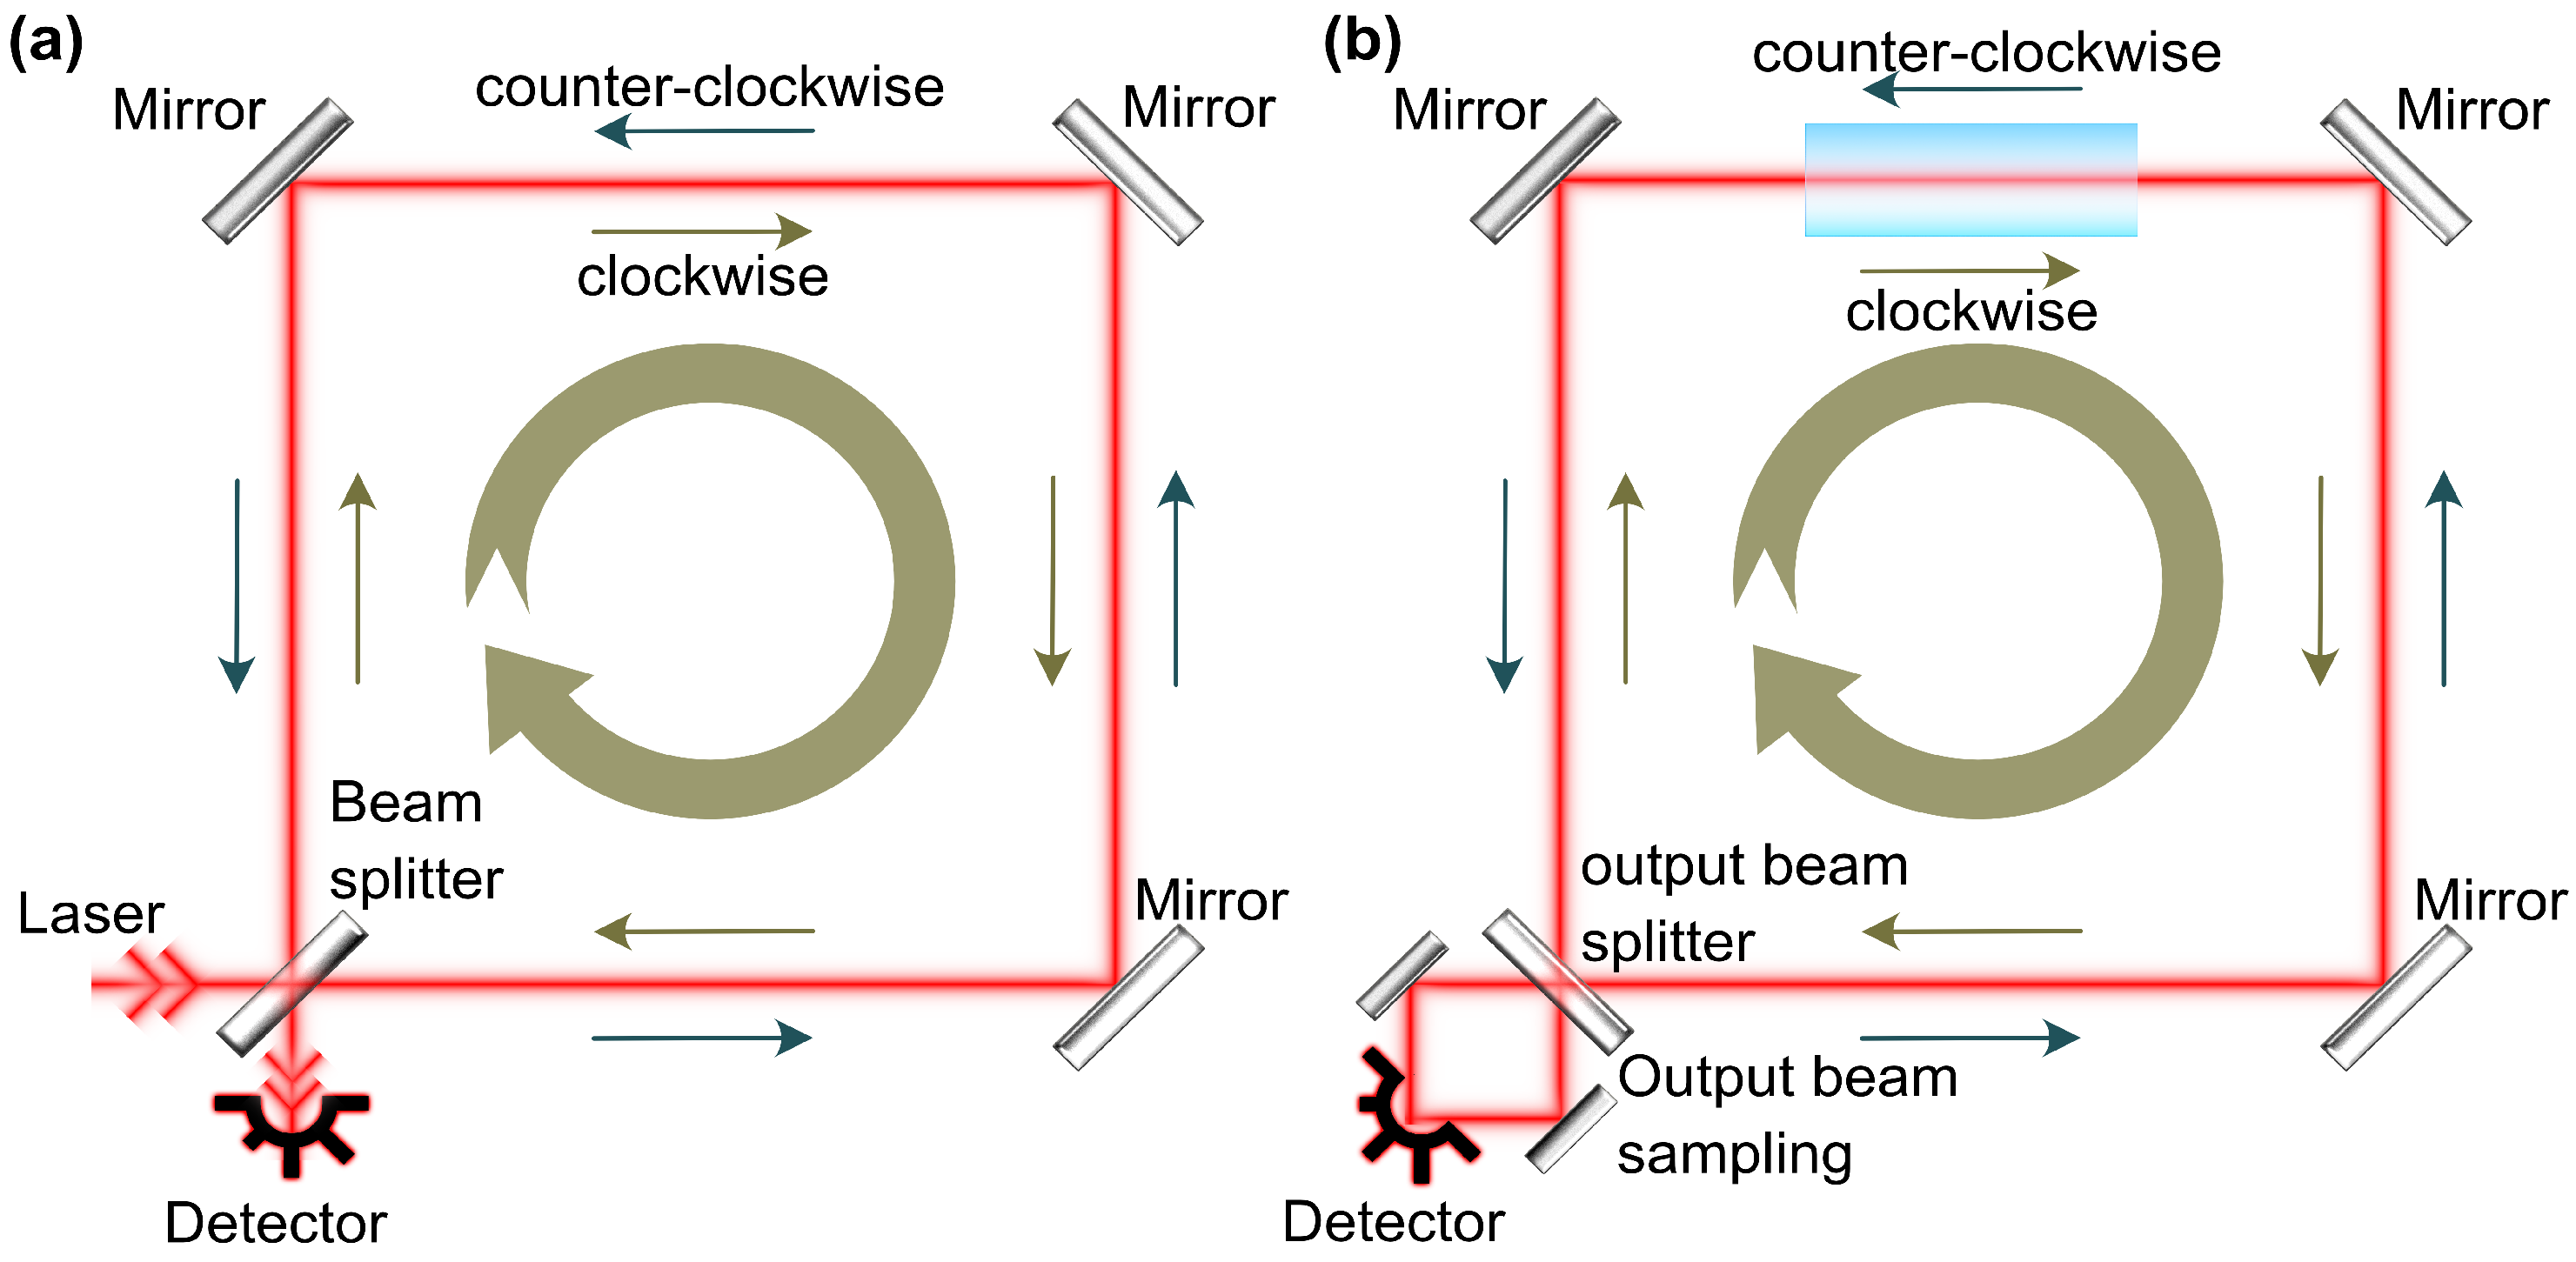
\includegraphics[width=0.6\columnwidth]{passive_active_gyroscope.png}
	\caption{Ring laser gyroscope systems. \textit{Left}: Passive, \textit{Right}: Active. Obtained from Ref. \cite{Kudelin2021}.}
	\label{fig:passive_active}
\end{figure*}

\subsubsection{Gyroscope Sensitivity}

The sensitivity of the ring laser gyroscope depends on a variety of factors, namely the wavelength $\lambda$, arm length $L$, finesse $F$
of the resonator (see Sec. \ref{sec:finesse}), and the shot-noise limited detection given by the number of photons $N = P_{\text{opt}} / h \nu = P_{\text{opt}} \lambda / hc$ detected per unit time. 
$P_{\text{opt}}$ represents the optical power given to the laser. Combining all such factors, we obtain the sensitivity of the ring laser gyroscope for an integration time $\tau$ as such: 
\begin{equation}
	\delta \Omega = \frac{1}{4} \frac{c}{L^2F}\sqrt{\frac{ch\lambda}{P_{\text{opt}}}} \frac{1}{\sqrt{\tau}}.
	\label{eq:gyroscope_sensitivity}
\end{equation}

This gyroscope sensitivity can be directly compared with the Allan deviation $\sigma_{\text{ad}}$ that determines the instability of 
a measurement for some averaged integration time $\tau$ (see Sec. \ref{sec:allan_dev}). 

\section{Optical Cavities}

A cavity is a hollow conductor which contains electromagnetic waves going in and reflecting off the walls. At certain frequencies, these reflected waves form standing waves which correspond to the resonant modes of the cavity. An optical cavity consists of an arrangement of mirrors, which produces standing electromagnetic waves. In our setup, instead of the traditional Fabry-P\'erot interferometer, which consists of two opposing flat mirrors, we use four mirrors. Nevertheless, the same principles of resonance modes applies.

\subsection{Cavity Modes}

The solution to optical resonators with parabolic mirrors and homogeneous medium is given by the Hermite-Gaussian modes. The Hermite-Gaussian modes are the solution to the paraxial Helmholtz equation, when considering Cartesian coordinates with the beam propagating along the $z$-axis (Fig. \ref{fig:hermite}.

\begin{figure}[htpb]
    \centering
    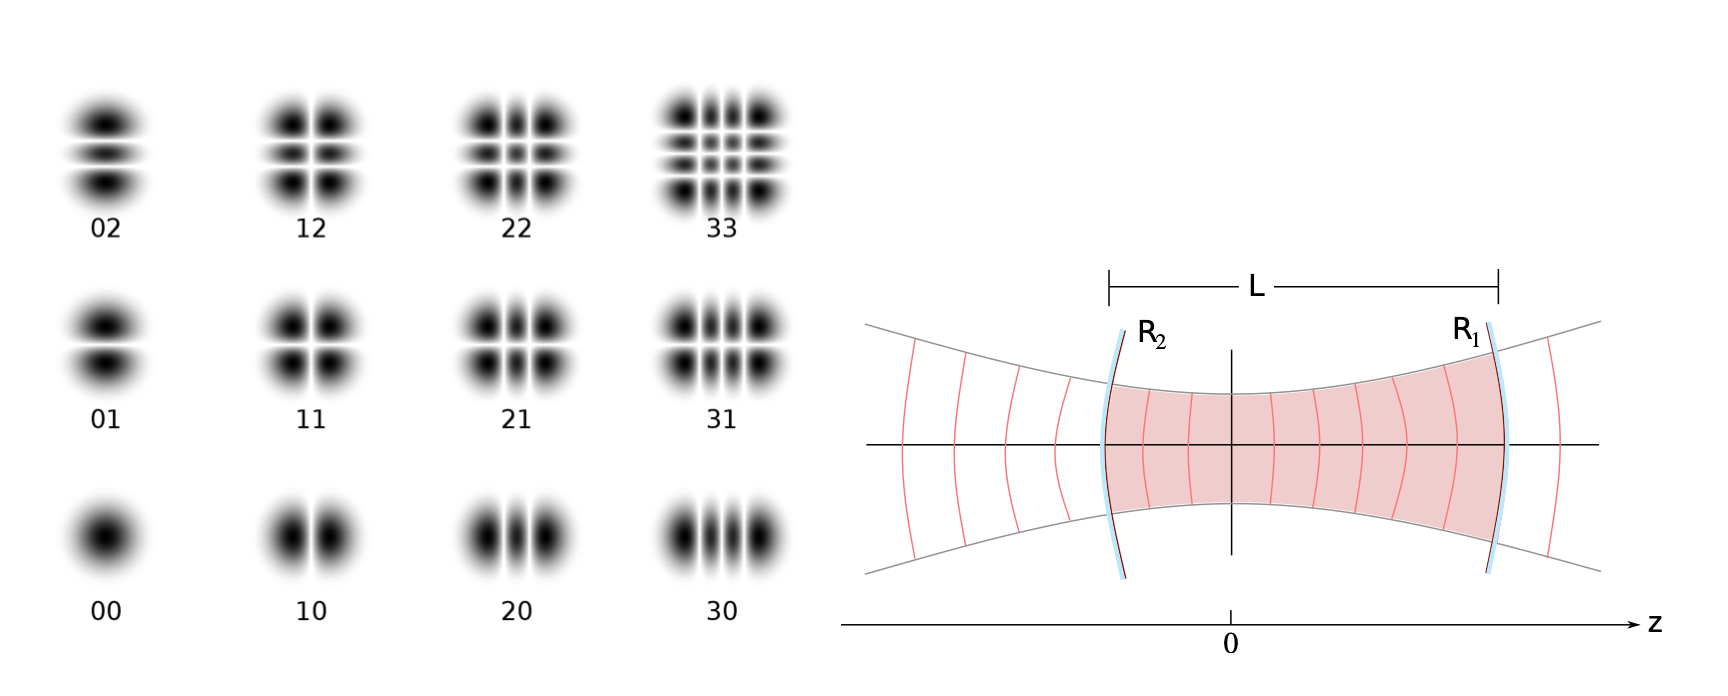
\includegraphics[width=0.8\textwidth]{hermite-gaussian}
	\caption{Hermite-Gaussian Transverse Electromagnetic Mode ($\mathrm{TEM}_{l, m}$) (left) and the beam's wavefront between two mirrors of radii $R_{1}$ and $R_{2}$ with a separation of length $L$, inside a cavity (right) \cite{Groh2021}. }
    \label{fig:hermite}
\end{figure}	

The Hermite-Gaussian modes are also called Transverse Electromagnetic Mode (TEM) and are labelled as $\mathrm{TEM}_{m,n}$, where $m, n \in \mathbb{N}^{\ge 0}$ are the integers, which represent the order of Hermite-polynomials along the $x$ and $y$ direction. The resonance frequency is given by

\begin{equation}
		\nu_{l, m, n} = \delta \nu_{\mathrm{FSR}}  \left(l + \left( m + n + 1 \right) \frac{\delta \zeta}{\pi  }\right) ,
\end{equation}
where $l \in \mathbb{N}^{\ge 0}$ represents the different longitudinal nodes. The spacing between these longitudinal modes is given by the free spectral range, $\delta \nu_{\mathrm{FSR}}$,

\begin{equation}
	\delta\nu_{\\mathrm{FSR}} = \frac{c}{P} .
	\label{eq:fsr}
\end{equation}

The fundamental mode, $\mathrm{TEM}_{0, 0}$ is the Gaussian mode and is used for locking the lasers beam in our setup, as can been seen in Fig. \ref{fig:tem00-lock}. In order to achieve stability, the following condition on the radii of two mirrors, $R_{1}$ and $R_{2}$, has to be met

\begin{equation}
		0 \leq g_{1}g_{2} = \left(1 + \frac{L}{R_{1}} \right)\left(1 + \frac{L}{R_{2}} \right) \leq 1.
\end{equation}
The above condition is true for a two mirror setup. In order to extend this to four mirror setup, we simply compute the magnitude of eigenvalues of ABCD transfer matrix for the roundtrip. 

\subsubsection{Airy Lineshape and Optical Cavity Ringing}
We expect the power transmitted through the cavity to have a Lorentzian like lineshape, called an Airy function, when the laser is scans through the frequencies of coupled modes. This occurs even with cavities with high Finesse cavities because the laser sweeps through different frequencies faster than the storage time of the cavity. This does not allow the cavity to recover and fill itself when resonance is approached. This leads to a beat, as the evolving field inside and the incoming field start to interfere and create an oscillatory behaviour. 

\subsection{Finesse} \label{sec:finesse}
The Finesse of a cavity essentially quantifies the number of bounces a beam makes before leaking out or being absorbed. Mathematically, it is the ratio of the free spectral range, $\delta \nu_{\mathrm{FSR}}$, to the spectral linewidth $\delta \nu_{1/2}$, the Full Width Half Maximum (FWHM) of the transmission peak. Since it is inversely proportional to the FWHM, a high finesse equals a narrow resonance line and vice versa. A narrow resonance line is better for high precision frequency applications. The formula is given by

\begin{equation} \label{eqn:finesse}
		\mathcal{F} = \frac{\delta \nu_{\mathrm{FSR}}}{\delta \nu_{1/2}} \approx \frac{\pi \sqrt{\mathcal{R}}}{1 - \mathcal{R}},
\end{equation}
where $\mathcal{R} = \sqrt{\mathcal{R}_{1} \mathcal{R}_{2} \mathcal{R}_{3} \mathcal{R}_{4}}$, where $\mathcal{R}_{i}$ is the reflectivity of the cavity mirrors. 

\subsection{Cavity-Ring-Down Technique} \label{sec:ring-down}
To precisely compute the finesse of mirrors in the cavity, we employ ring-down technique. In this, we look at how the power in the cavity evolves temporally, when the cavity-locked laser is switched off quickly. In order to achieve the latter, we switch the RF signal driving the Acousto-Optical Modulator (AOM). 

Neglecting the losses in the cavity medium, the time evolution of the laser intensity is given by

\begin{equation}
		\label{eqn:ring-down}
		I(t) = I_{0}\mathcal{R}^{2t/\tau _{r}} = I_{0} \exp\left(-\frac{t}{\tau _{dec}}\right),
\end{equation}
where $\tau _{r} = P /c $ is the roundtrip time and $\tau _{dec}$ is the decay time, which is given by

\begin{equation}\label{eqn:reflec}
		\tau _{dec} = -\frac{\tau _{r}}{\log \mathcal{R}^2} = - \frac{P}{c \log \mathcal{R}^2}.
\end{equation}

\subsection{Pound-Drever-Hall Locking}
Pound-Drever-Hall (PDH) technique is a way to stabilize the frequency of light emitted by the laser by locking to a stable cavity. The central idea of this technique is the following - phase modulated light, typically by an Electro-Optical Modulator (EOM), consisting of carrier frequency $\omega$ and two side bands $\Omega$ is inserted into the cavity. The reflected light from the cavity is recorded with a fast photodiode, which consists of the two unaltered side bands and a phase shifted carrier. This phase shifted carrier is mixed with the local oscillator and passed through a low pass filter in order to remove high frequency components. The resulting signal shows how far off the laser carrier is from resonance. This signal is then fed into the Proportional-Integral-Derivative (PID) controller, which then applies an error signal (Fig. \ref{fig:error-signal}) and which is then fed back into the cavity, allowing the laser to remain locked.

\begin{figure}[htpb]
    \centering
    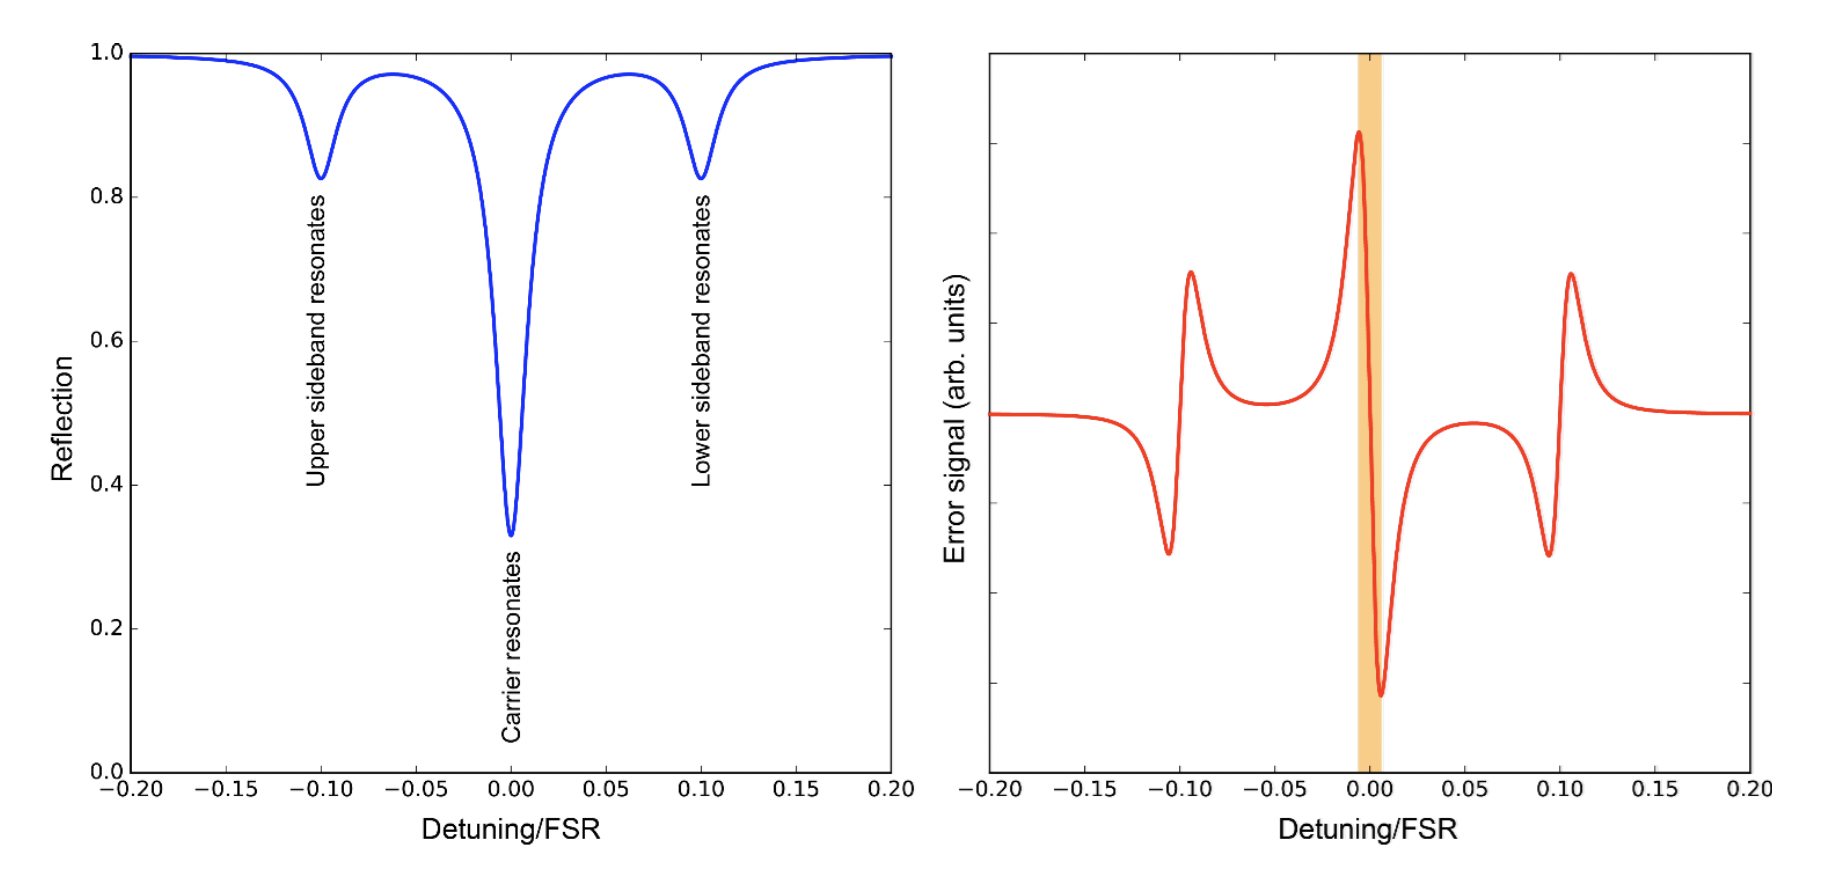
\includegraphics[width=0.8\textwidth]{error-signal}
	\caption{Pound-Drever-Hall (PDH) cavity reflection (left), which shows the ingoing carrier frequency along with two sidebands. The error signal after frequency demodulation (right) that is used for PID feedback to stabilize the laser \cite{pdhmanual}.}
    \label{fig:error-signal}
\end{figure}

To the first order, the frequency components can be approximated to: 

\begin{equation}
		E_{\mathrm{in}} = E_{0} e^{i \left(\omega t + \beta \sin(\Omega t) \right) } \approx E_{0} \left(J_{0} (\beta) e^{i \omega t } + J_{1}(\beta) e^{i(\omega + \Omega) t} - J_{1}(\beta) e^{i (\omega - \Omega)t} \right),
\end{equation}
where $J_{k}$ are the Bessel functions and $\beta$ is the modulation depth. The reflection coefficient is give by $F(\omega) = E_{\mathrm{ref}} / E_{\mathrm{in}}$.

The slope of the error signal is given by

\begin{equation}
		\epsilon \propto - \frac{4}{\pi} \sqrt{P_{c} P_{s}} \delta \nu _{1/2}, 
\end{equation}
where $P_{c}$ is the carrier power given by $P_{c} = J_{0}^2 (\beta) \left| E_{0}^2 \right| $ and $P_{s}$ is the sideband powder which is given by $P_{s} = J_{1}^2 (\beta) \left| E_{0}^2 \right| $.
Selecting good PID parameters for correcting both fast and slow laser lock disturbances can help achieve frequency stabilization to a fraction of the cavity linewidth. 

\subsection{Lock-In Effect} \label{sec:lockin_effect}
The lock-in effect occurs when the two oscillator modes with a small delta frequency between them start oscillating at the same frequency due to weak coupling between them. This is a common occurrence in the field of physics and the best example are two oscillating pendulums hung upon the same wooden wall, oscillating with slightly different frequency eventually synchronize and start oscillating at the same frequency. In general, the frequency difference between two pendulums is, 

\begin{equation}
		\delta f = \sqrt{f_{0}^2 - f_{L}^2},
\end{equation}
where $f_{L}$ is the lock-in threshold below which the two pendulums synchronize. This effect can also be seen in RF electronics and optics. 

In our setup, we can encounter this phenomenon due to the back scattering losses in the mirrors of the cavity, which is usually only a few ppm, but can amplified due to presence of dust. These losses lead to a delta in the frequency, which leads to the lock-in effect. The lock-in threshold is given by

\begin{equation}
		\Omega_{L} = \frac{c \lambda^2 r_{s}}{32 \pi  A d},
		\label{eq:lockin_thresh}
\end{equation}
where $\lambda$ is the laser wavelength, A is the enclosed area of the cavity, d is the cavity mode beam diameter and $r_{s}$ the fraction of backscattering as compared to other losses \cite{Liu}.

With the present setup, the lock-in threshold is much greater than the Earth rotation, which will limit our ability to measure it accurately. In order to reduce the locking threshold, a larger ring and reduced scattering losses will be required. 

\section{Allan Deviation} \label{sec:allan_dev}

The Allan deviation is used to quantify the instability of any device that measures differences in frequencies. Assuming that the
measurement is only limited by the photon shot-noise (amongst others), we can describe the Allan variance as the deviation
between temporal averages of measurements $y$ over some time interval or integration time $\tau$:
\begin{equation}
	\sigma_{{\text{ad}}}^2 = \frac{1}{2M} \sum\limits_{n=1}^M (\bar{y}(\tau)_{n+1} - \bar{y}(\tau)_n)^2,
	\label{eq:allan_def}
\end{equation}
where $M$ is the number of samples. The Allan deviation is then the square root of the variance. \par 

The Allan deviation is especially helpful to understand the sensitivity in gyroscopes. Imposing the same assumptions as above,
we can describe the Allan deviation with typical shot noise scaling $\propto 1 / \sqrt{\tau}$ as such:
\begin{equation}
	\sigma_{\text{ad}} = \mathcal{A} \tau ^ m = \frac{\mathcal{A}}{\sqrt{\tau}},
	\label{eq:allan_shotnoise}
\end{equation}
where $\mathcal{A}$ (given in $\si{\radian\per\second\per\sqrt{\hertz}}$) is known as the shot-noise limited sensitivity of the gyroscope and $m = -\frac{1}{2}$ \cite{Groh2021}. \par 

To compare this value to the sensitivity of the laser gyroscope, we use the relation between the Sagnac frequency and the 
rotation rate given in Eq. \ref{eq:Sagnac_scale} and evaluate the Allan deviation at the shot-noise time interval $\tau_{\mathrm{sn}}$:
\begin{equation}
	\delta \Omega_{\mathrm{ad}} = \frac{\sigma_{\text{ad}} (\sqrt{\tau_{\mathrm{sn}}})}{n} = \frac{\mathcal{A}}{\sqrt{\tau_{\mathrm{sn}}}n} . 
	\label{eq:allan_sensitivity}
\end{equation}



\chapter{Pre-Lab Exercises}

Before conducting the experiment, we were required to determine the rotation rate of the Earth using our phone. Our phones
contain a microelectromechanical system (MEMS), which is a portable and inexpensive inertial sensor that track the motion of
the phone. Using the application \texttt{phyphox} constructed by RWTH Aachen University, we evaluated the capabilities
of the MEMS gyroscope within our phones. 

\section{Task 1: Getting Started}

We downloaded the \texttt{phyphox} app made by RWTH Aachen University, and we played around with the Gyroscope function. We rotated the phone in several directions 
to observe the relationship between the orientation of the phone and the corresponding coordinates used in the application. This is shown in Fig. \ref{fig:phone_sketch}. 
Fig. \ref{fig:gyro_plot_z} - \ref{fig:gyro_plot_x} show the corresponding time series for the $x, y, z$ coordinates for each rotation that we performed. 

\begin{figure*}[hbt!]
	\centering
	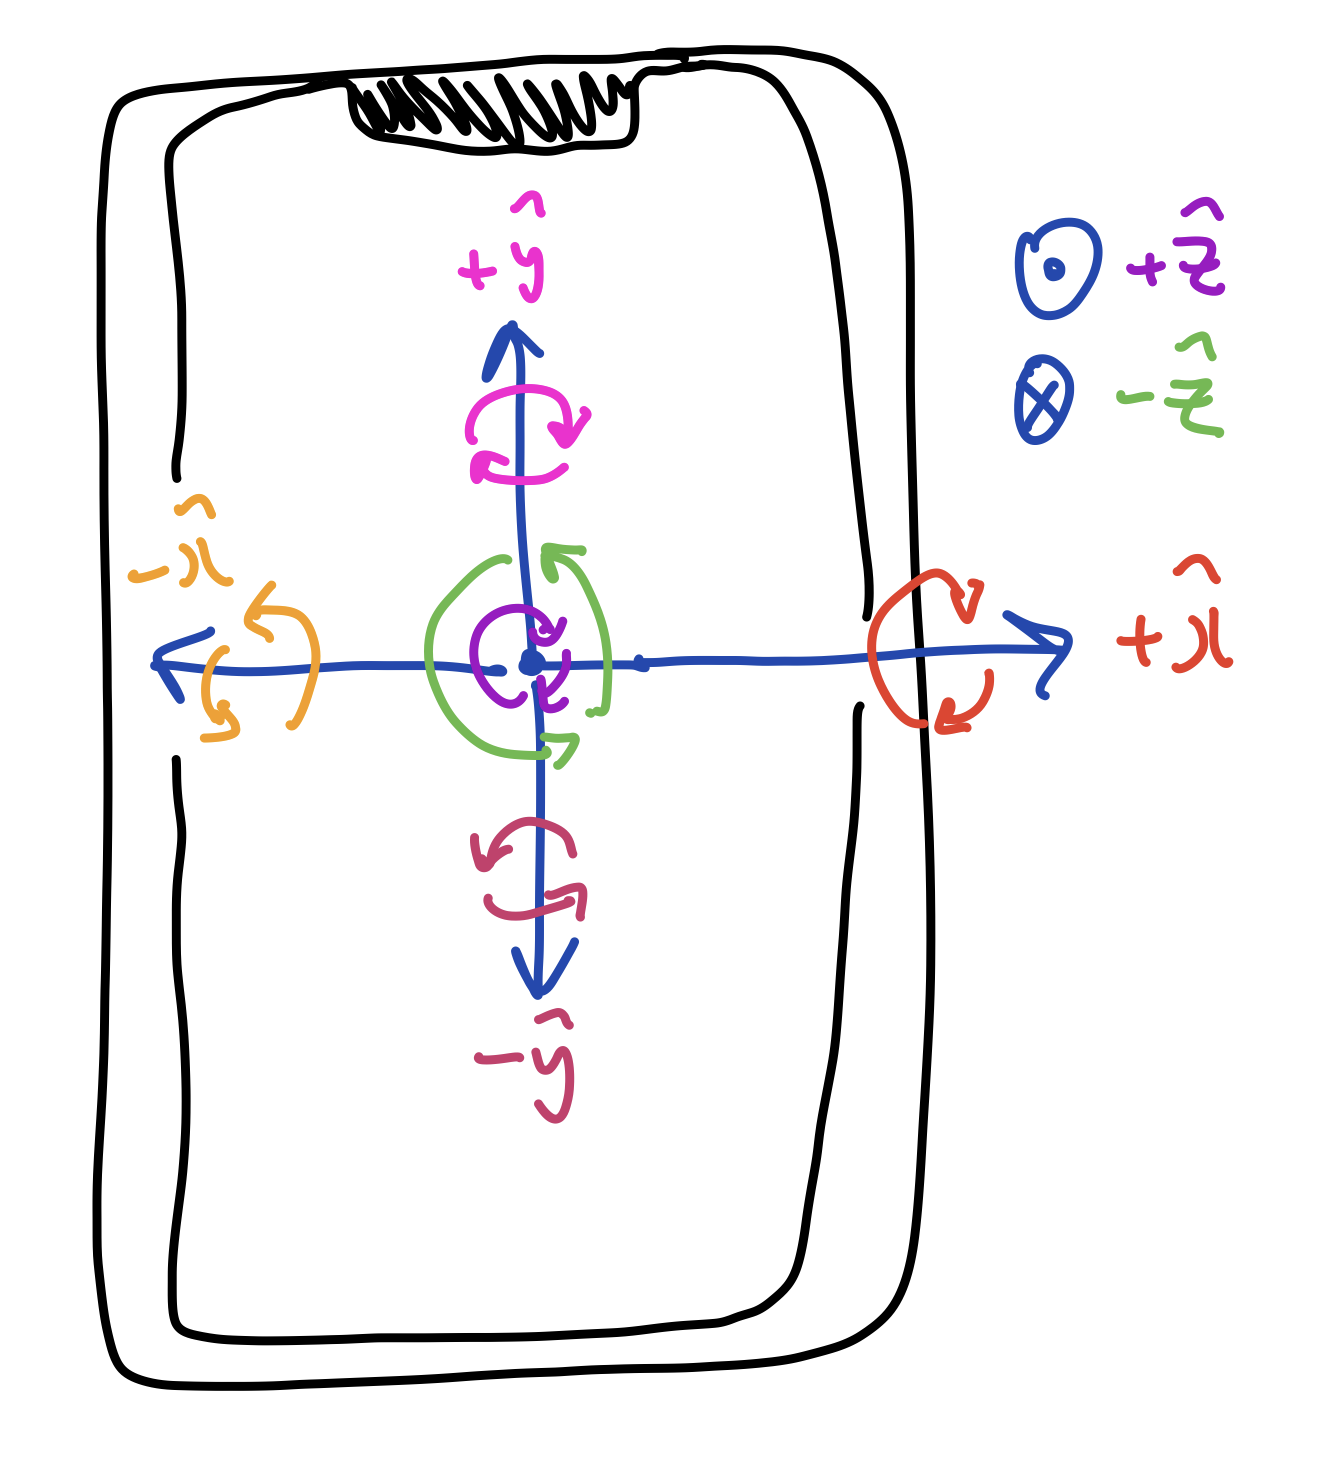
\includegraphics[width=0.6\columnwidth]{Phone_sketch.png}

	\caption{Sketch of the phone used to measure the gyroscope with its relevant $x, y, z$ coordinates and sense of rotation. 
            The sense of rotation is color coded with each rotation axis, and the direction of the axis is indicated by the blue arrows.}
	\label{fig:phone_sketch}
\end{figure*}

\begin{figure*}[hbt!]
	\centering
	\subfloat[$+z$ direction, anti-clockwise]{{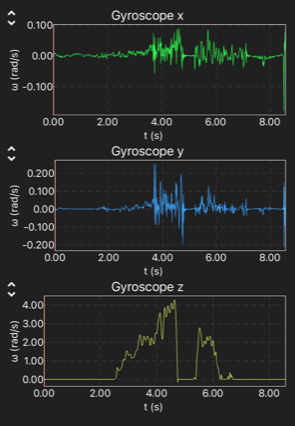
\includegraphics[width=0.3\columnwidth]{rotation_posz.PNG}}}
	\quad
	\subfloat[$-z$ direction, clockwise]{{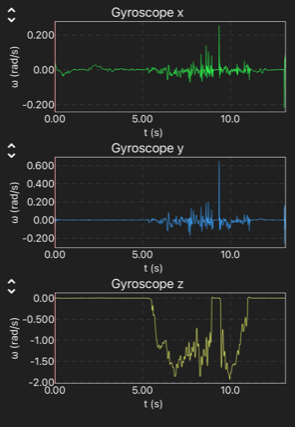
\includegraphics[width=0.3\columnwidth]{rotation_negz.PNG}}}

	\caption{The time series of the $x, y, z$ coordinates shown from the \texttt{phyphox} application when 
            the phone was rotated parallel to the surface. This corresponds to rotations in the $z$-direction. Note the large amplitudes in 
            the time series, which indicates rotations in the relevant axis. }
	\label{fig:gyro_plot_z}
\end{figure*}


\begin{figure*}[hbt!]
	\centering
	\subfloat[$+y$ direction, into surface (anti-clockwise)]{{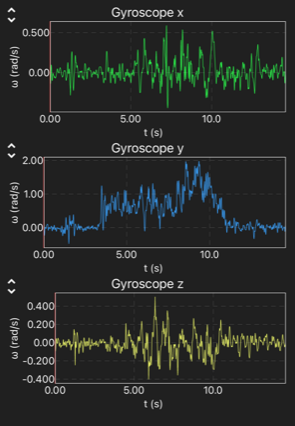
\includegraphics[width=0.3\columnwidth]{rotation_posy.PNG}}}
	\quad
	\subfloat[$-y$ direction, out of surface (clockwise)]{{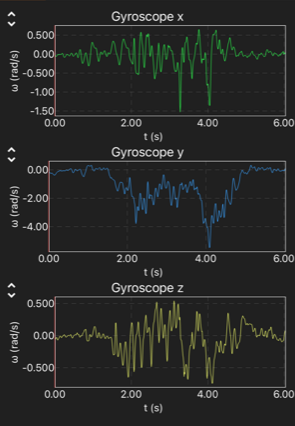
\includegraphics[width=0.3\columnwidth]{rotation_negy.PNG}}}

	\caption{Same as Fig. \ref{fig:gyro_plot_z} but for rotations into / out of the surface, corresponding to rotations in $y$-direction.}
	\label{fig:gyro_plot_y}
\end{figure*}


\begin{figure*}[hbt!]
	\centering
	\subfloat[$+x$ direction, rotation towards user (anti-clockwise)]{{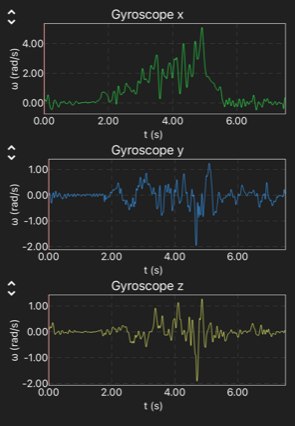
\includegraphics[width=0.3\columnwidth]{rotation_posx.PNG}}}
	\quad
	\subfloat[$-x$ direction, rotation away from user (clockwise)]{{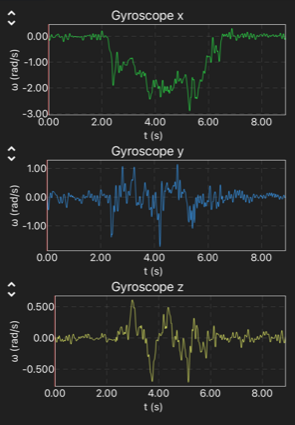
\includegraphics[width=0.3\columnwidth]{rotation_negx.PNG}}}

	\caption{Same as Fig. \ref{fig:gyro_plot_z} but for rotations towards / away the user, corresponding to rotations in $x$-direction.}
	\label{fig:gyro_plot_x}
\end{figure*}

To save the rotation rates and import it into the computer for further analysis, the \texttt{Export Data} feature can be utilized. This will save the 
data as a \texttt{.zip} file that contains the raw data, the software and specifics regarding the device used, and the system time in which the experiment was 
started and finished. All such files are saved as \texttt{.csv} formats. An example for the raw data is shown in the Appendix section.\par 

To obtain a faster rotation rate, we applied maximal torque on each end of the phone such that the rotation at each axis was maximal. This was done at an adequate height
to ensure the rotation rate was properly measured. Several cushions were placed on top of a bed to ensure that the phone does not break. Fig. \ref{fig:gyro_plot_fast} show
the time series of the $x, y, z$ coordinates in the $+y$ and $-z$ directions. Performing the measurement in such a way yields a more notable and stable measurement of the rotation rate 

\begin{figure*}[hbt!]
	\centering
	\subfloat[$+y$ direction \label{fig:gyro_plot_fast_y}]{{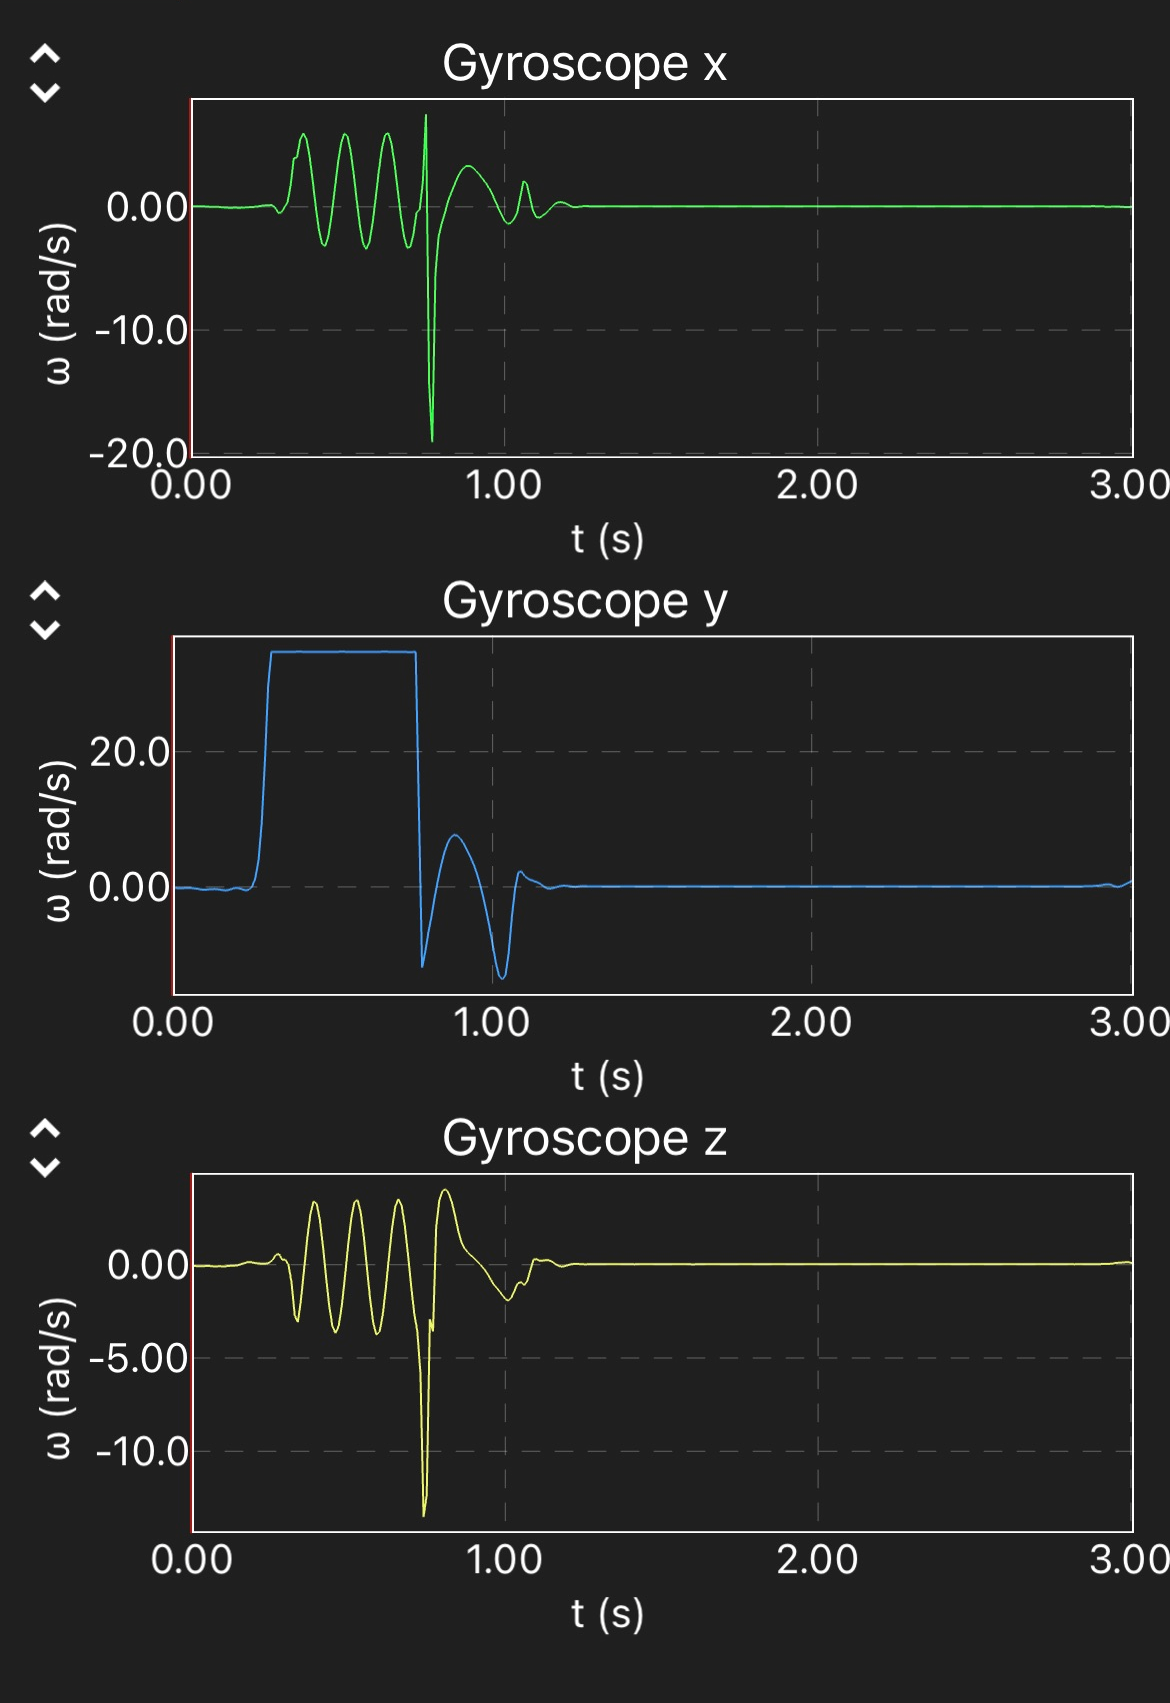
\includegraphics[width=0.3\columnwidth]{rot_fast_posy.png}}}
	\quad
	\subfloat[$-z$ direction \label{fig:gyro_plot_fast_z}]{{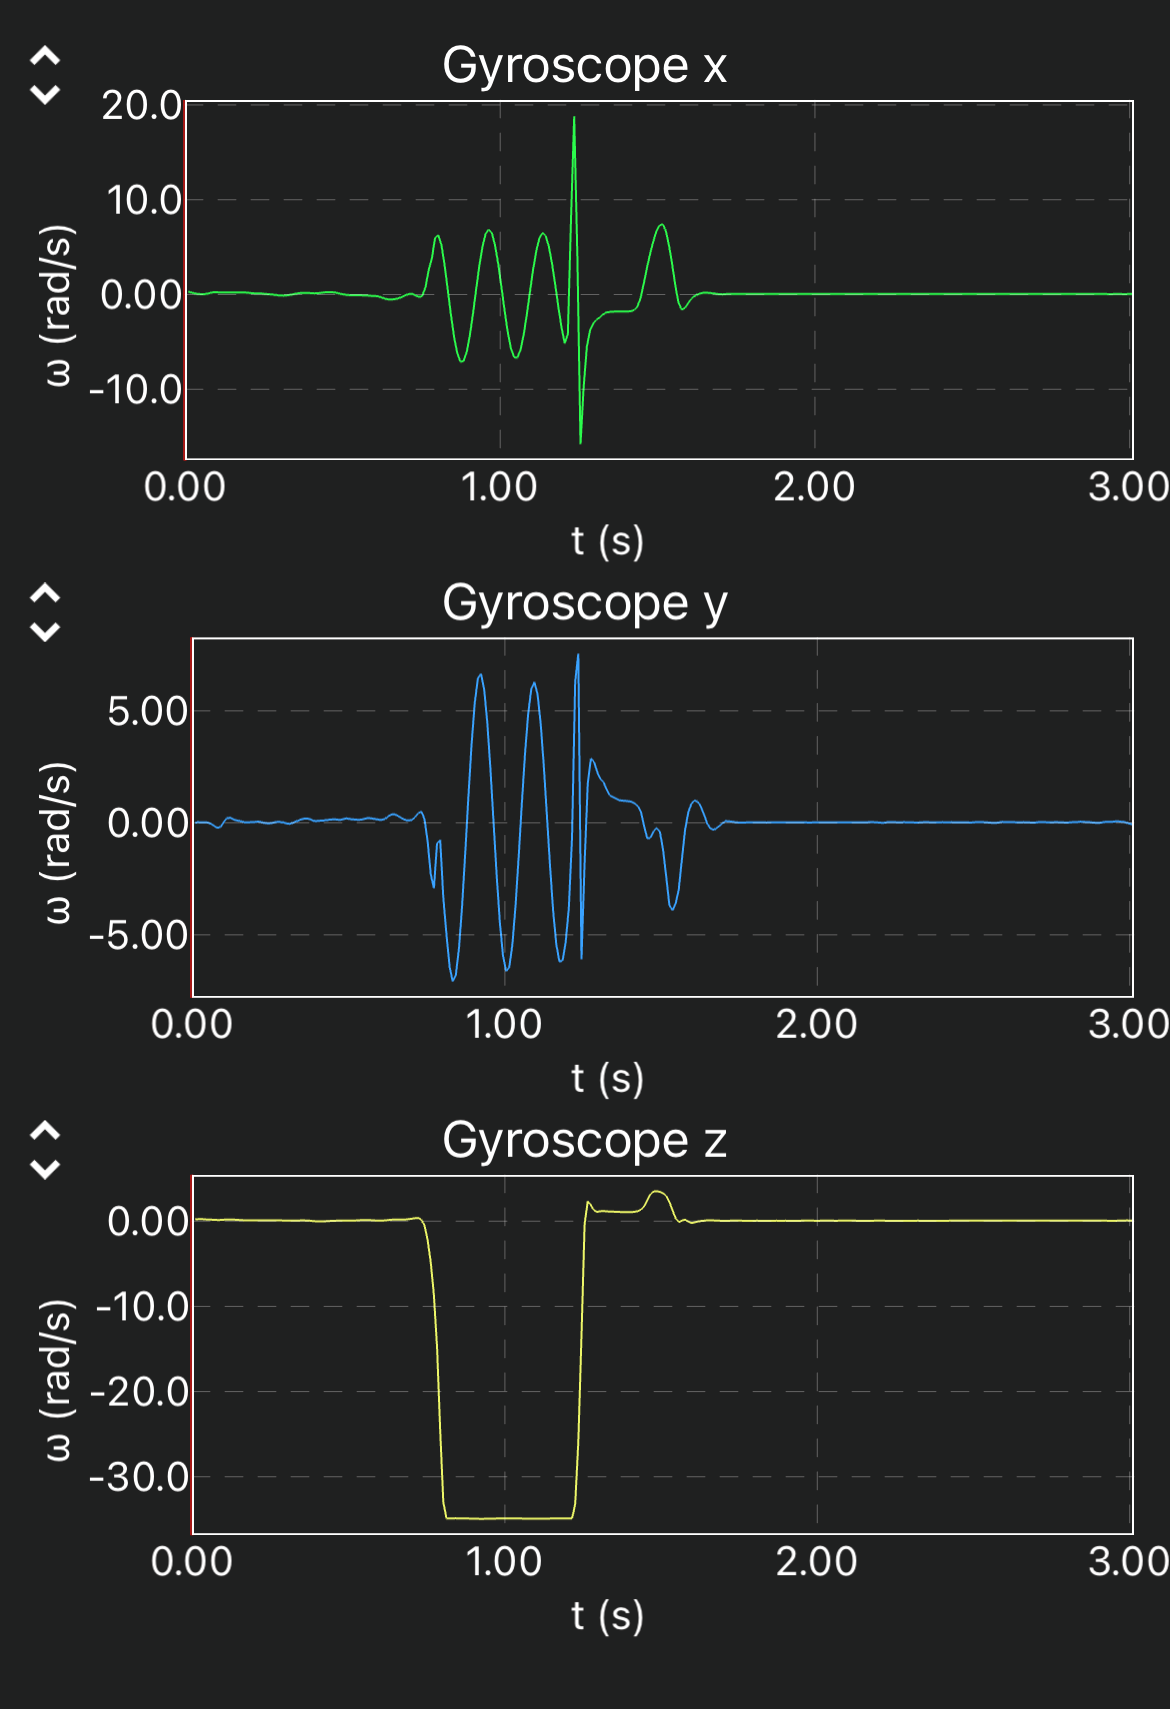
\includegraphics[width=0.3\columnwidth]{rot_fast_negz.PNG}}}

	\caption{Same as Fig. \ref{fig:gyro_plot_z} but for fast rotations in the (a) $+y$ and (b) $-z$ direction.}
	\label{fig:gyro_plot_fast}
\end{figure*}


\section{Task 2: Allan Deviation} \label{sec:prelab_allan_dev}

To determine the Allan deviation of the phone's MEMS gyroscope, we placed our phone on a platform with minimal disturbance and 
took the measurement for approximately one hour. Fig. \ref{fig:prelab_allan_time} shows the time series for each gyroscopic 
component obtained. From the time series alone, we observe that there are no significant deviations in the measurements in 
each direction. \par 

\begin{figure*}[h!]
	\centering
	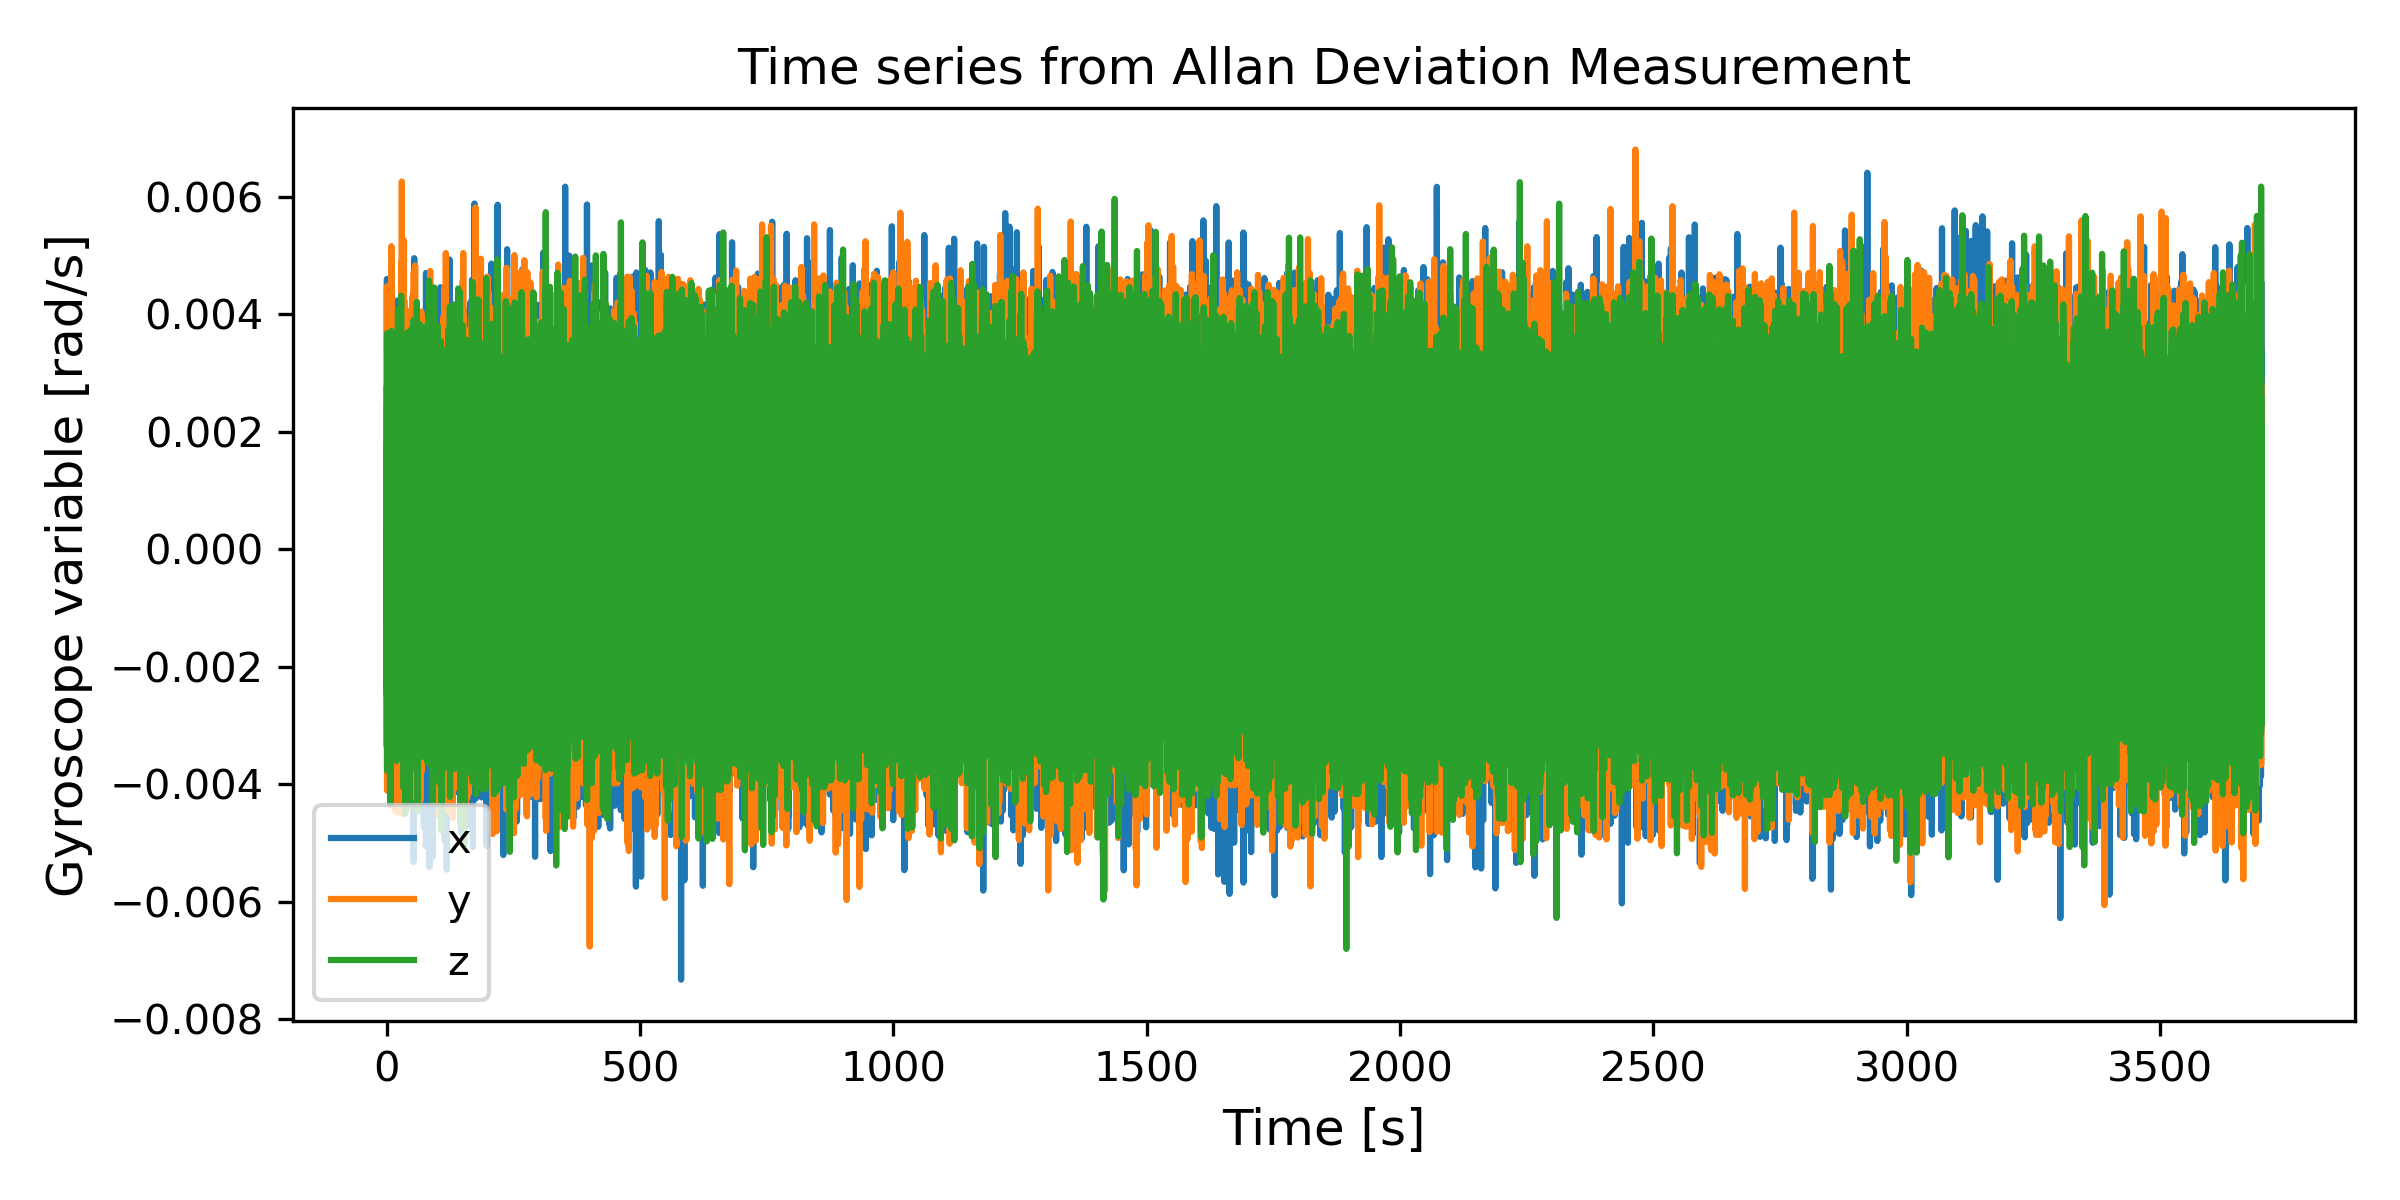
\includegraphics[width=0.75\columnwidth]{prelab_allan_time_series.png}

	\caption{Time series of the Allan deviation measurement for each gyroscopic component.}
	\label{fig:prelab_allan_time}
\end{figure*}

We then performed a Fast Fourier Transform (FFT) using the built-in package \texttt{scipy.fft} to obtain the plot in the frequency
domain. Fig. \ref{fig:prelab_allan_fourier} shows the Fourier spectrum in each gyroscopic component. We observe that up until around
a frequency of $\SI[]{1.5}[]{\hertz}$, the frequency spectrum shows the noise of the measurement. After this point, we observe 
that the spectrum drops significantly, which indicates that the gyroscope readings occur after this point in the frequency domain. 
We observe that there is a dip in the spectrum at around $\SI{2.2}{\hertz}$ as well as a small peak at approximately 
$\SI{18}{\hertz}$ for the measurement in the x direction. This may be caused by the 
location in which the MEMS gyroscope is placed within the phone, which would account for the bias in the x direction. We observed the 
same phenomena when measuring for the rotation rate of the Earth, indicating a clear bias in the x direction. \par 

\begin{figure*}[h!]
	\centering
	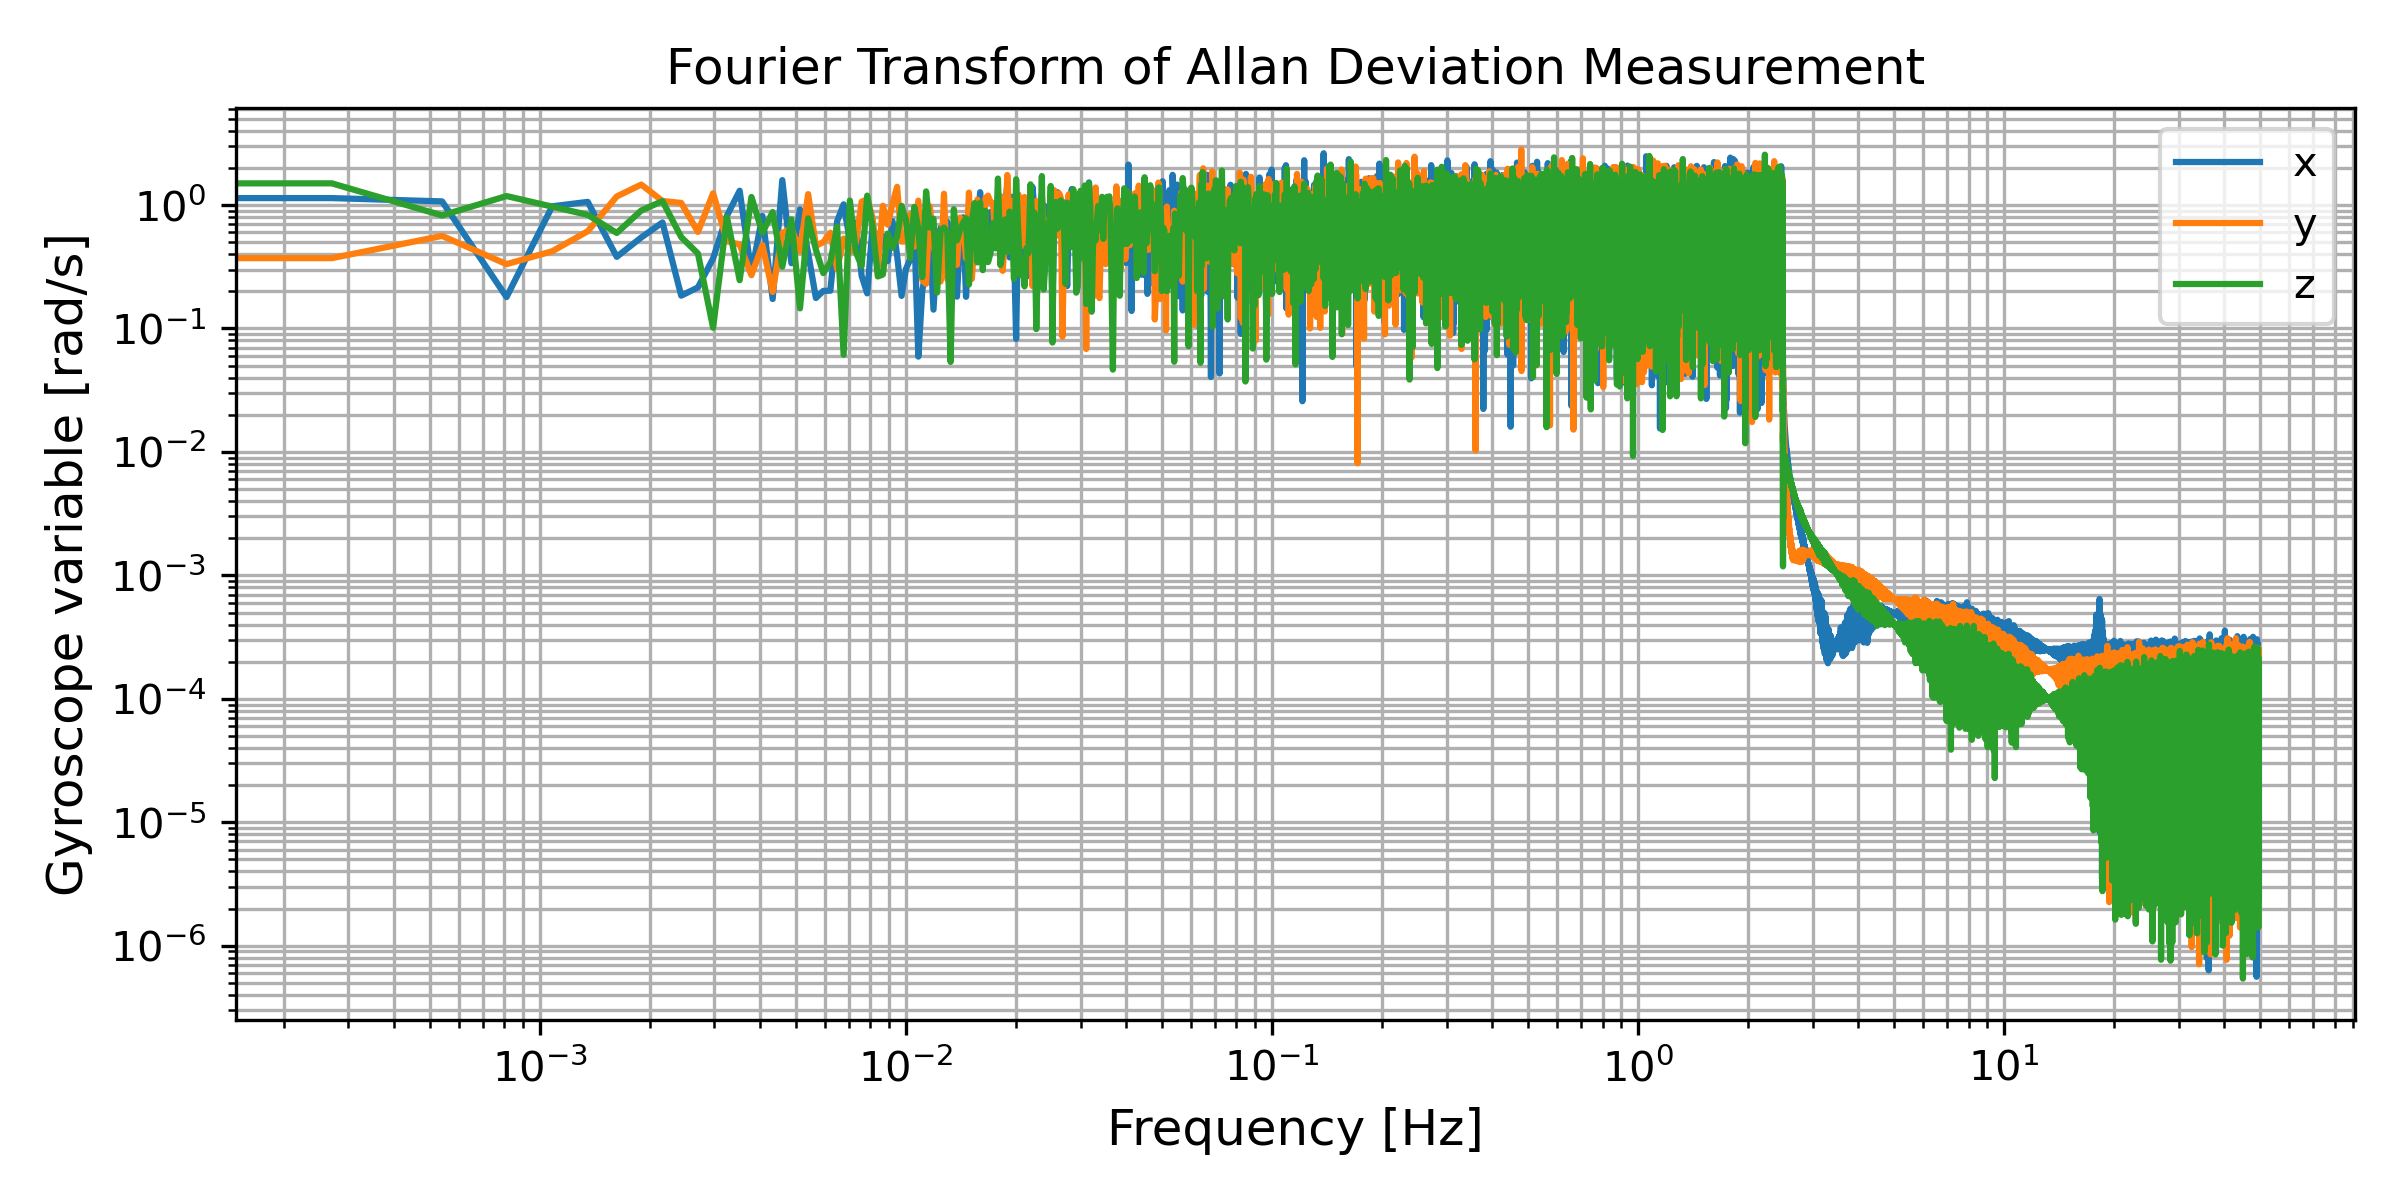
\includegraphics[width=0.75\columnwidth]{prelab_allan_fourier.png}

	\caption{The Fourier spectrum of the Allan deviation measurement in each gyroscopic direction.}
	\label{fig:prelab_allan_fourier}
\end{figure*}

To determine the Allan deviation, we used the function \texttt{oadev} from the Python package \texttt{allantools} 
that computes the overlapping Allan deviation given the frequency data, the sample rate, and the time series of the measurement. This returns
the Allan deviation for each integration time $\tau$. By using \texttt{oadev} instead of the standard \texttt{adev}, the noise that is 
apparent after the point of instability is reduced, yielding a smooth curve at each integration time. The sampling rate was obtained by taking the inverse of the timestep in the 
measurement, yielding a sampling rate of $\SI[]{99.2}[]{\hertz}$. Fig. \ref{fig:prelab_allan} shows the Allan deviation for each gyroscopic component 
at each integration time, displayed in a log-log format. \par 

\begin{figure*}[hbt!]
	\centering
	\subfloat[$x$ direction \label{fig:prelab_allan_x}]{{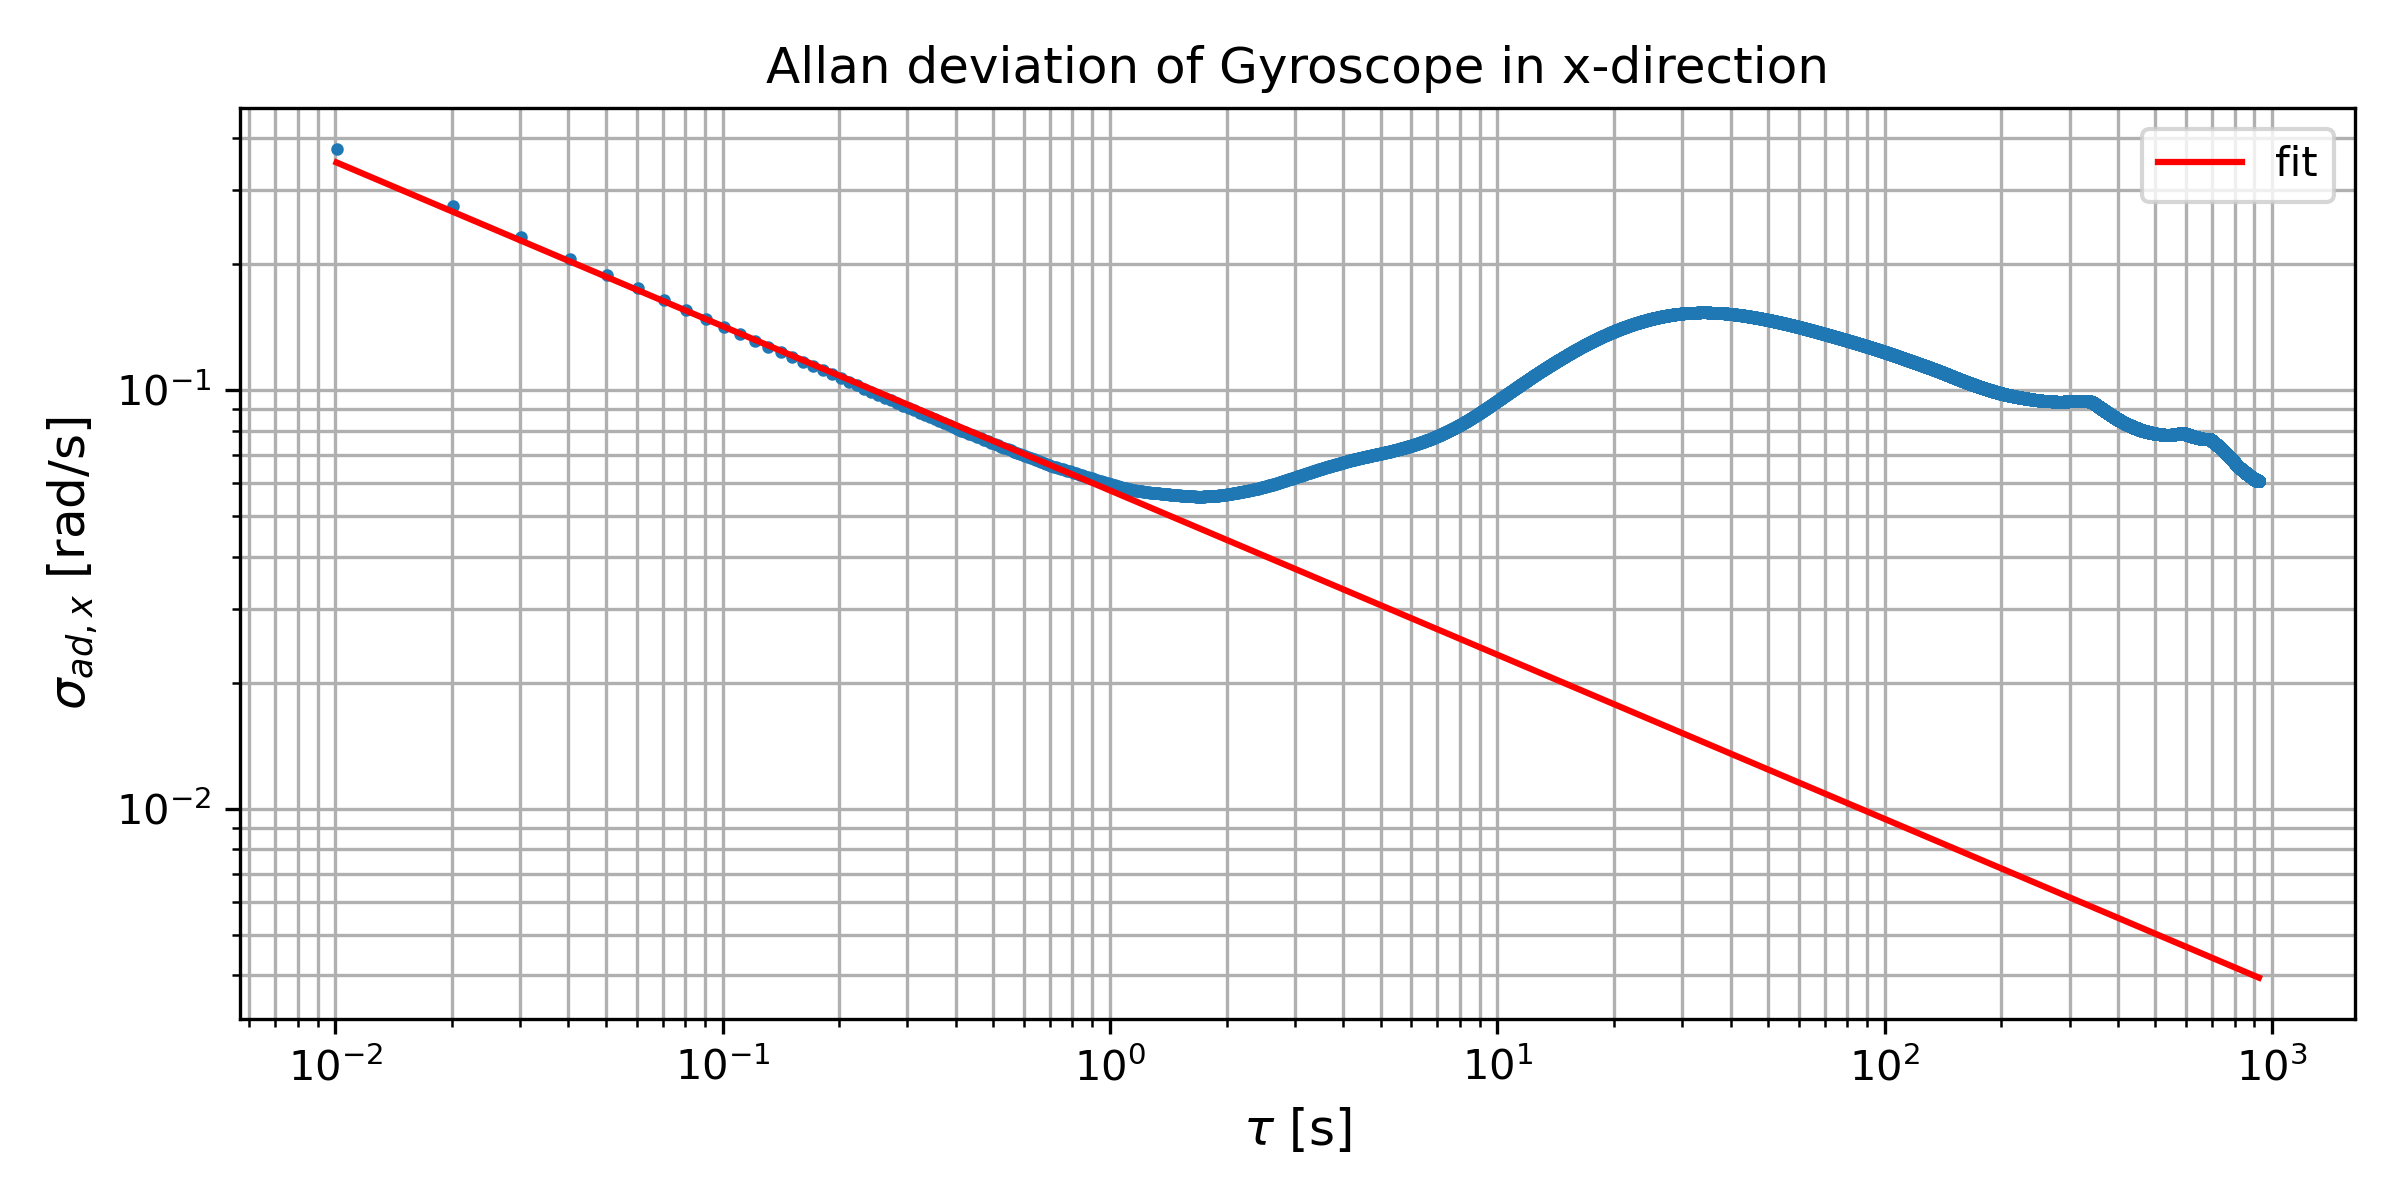
\includegraphics[width=0.7\columnwidth]{prelab_allan_x.png}}}
	\quad
	\subfloat[$y$ direction \label{fig:prelab_allan_y}]{{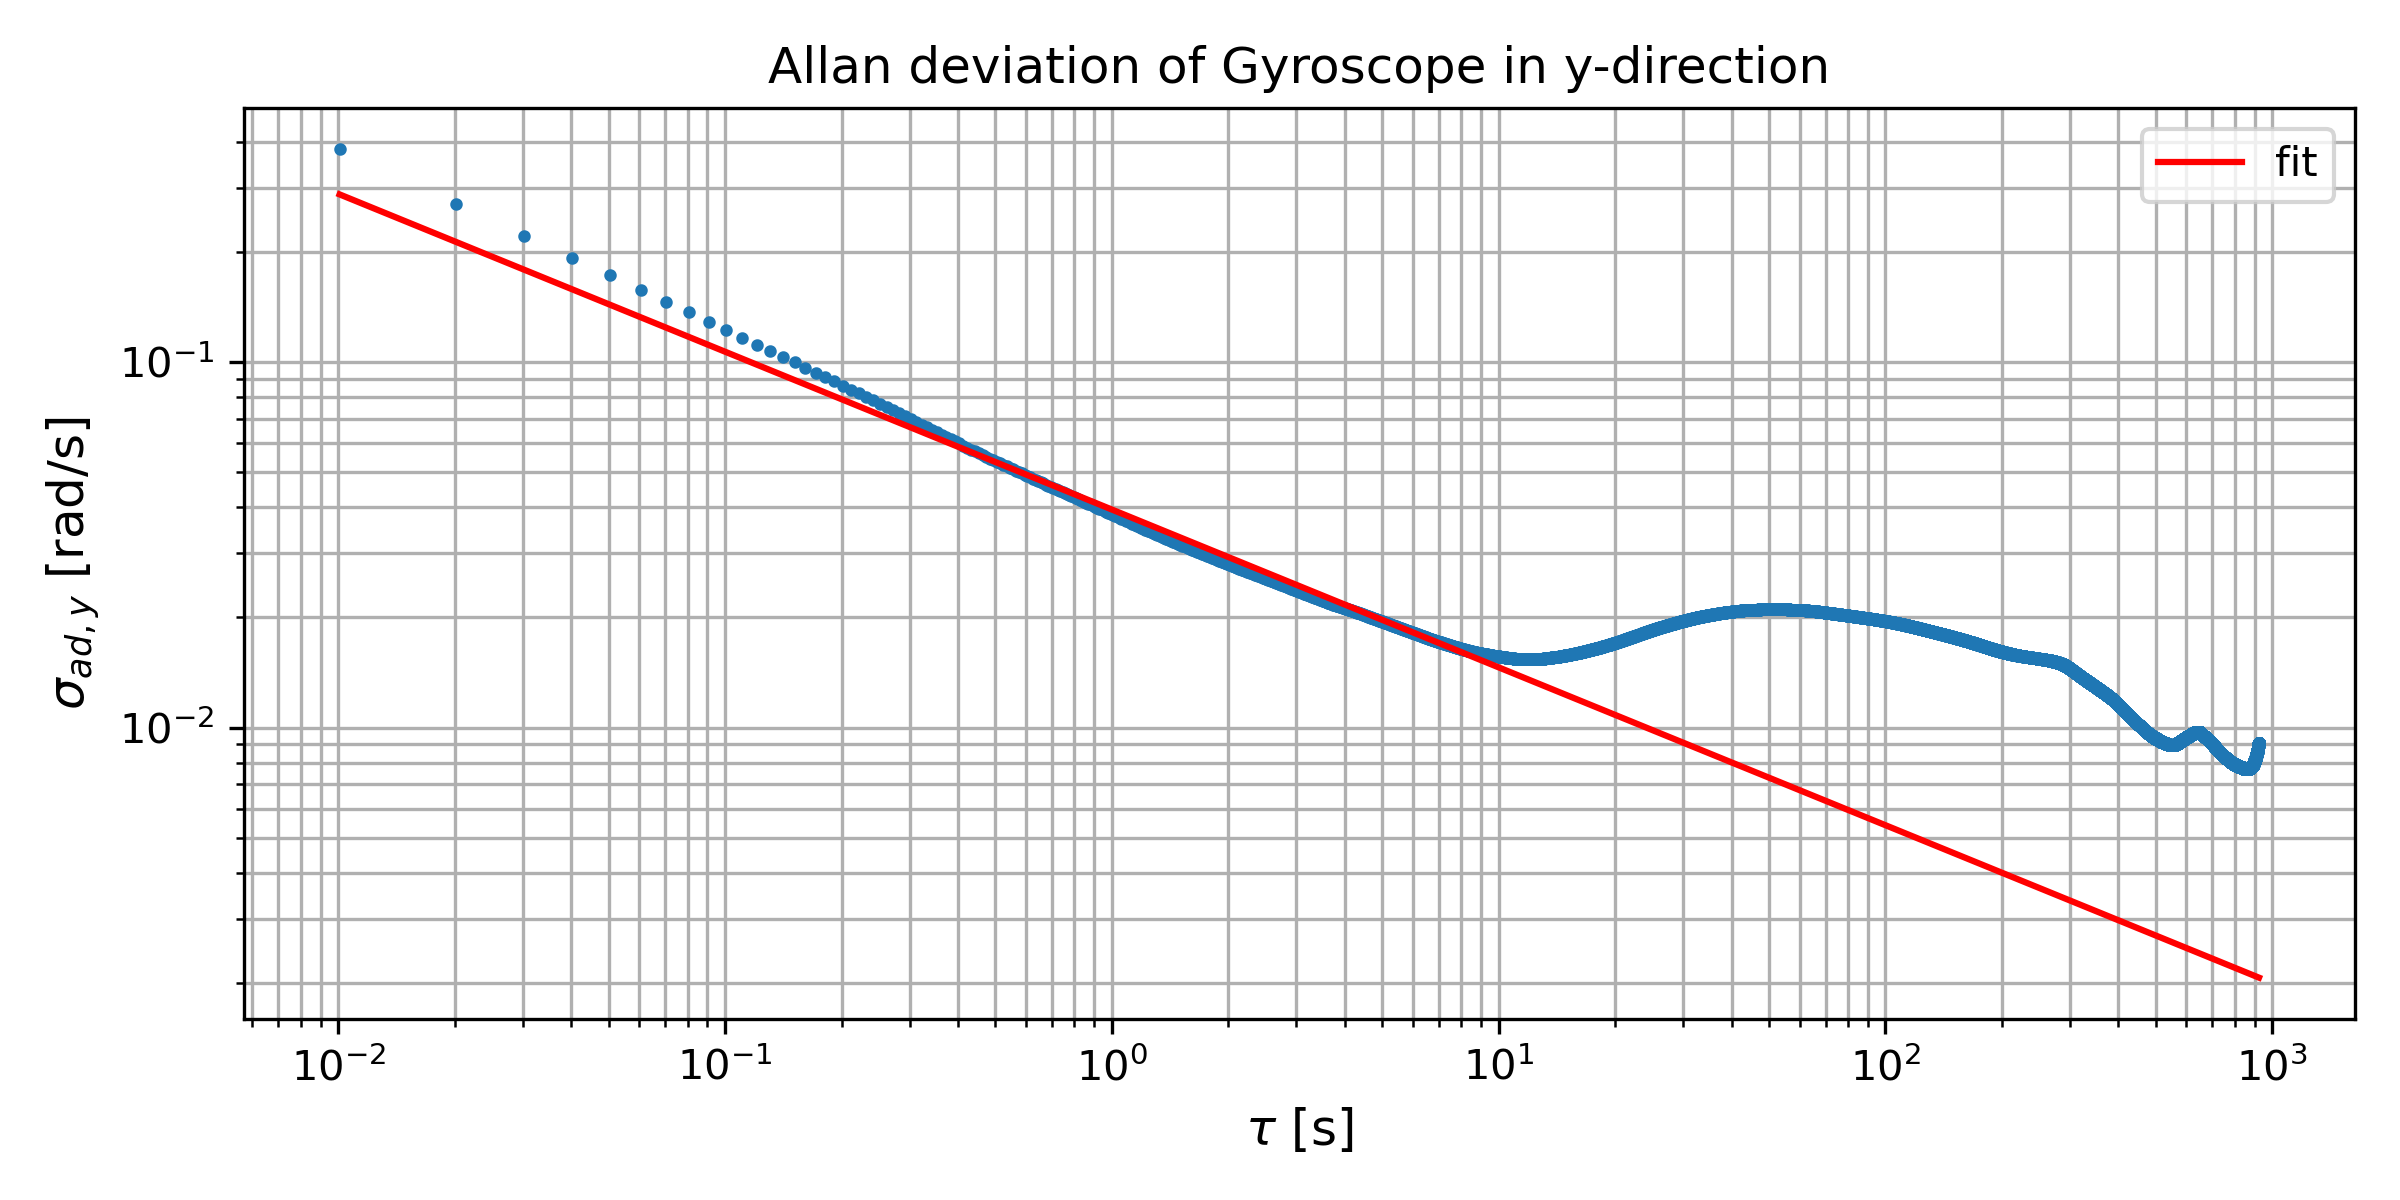
\includegraphics[width=0.7\columnwidth]{prelab_allan_y.png}}}
	\quad
	\subfloat[$z$ direction \label{fig:prelab_allan_z}]{{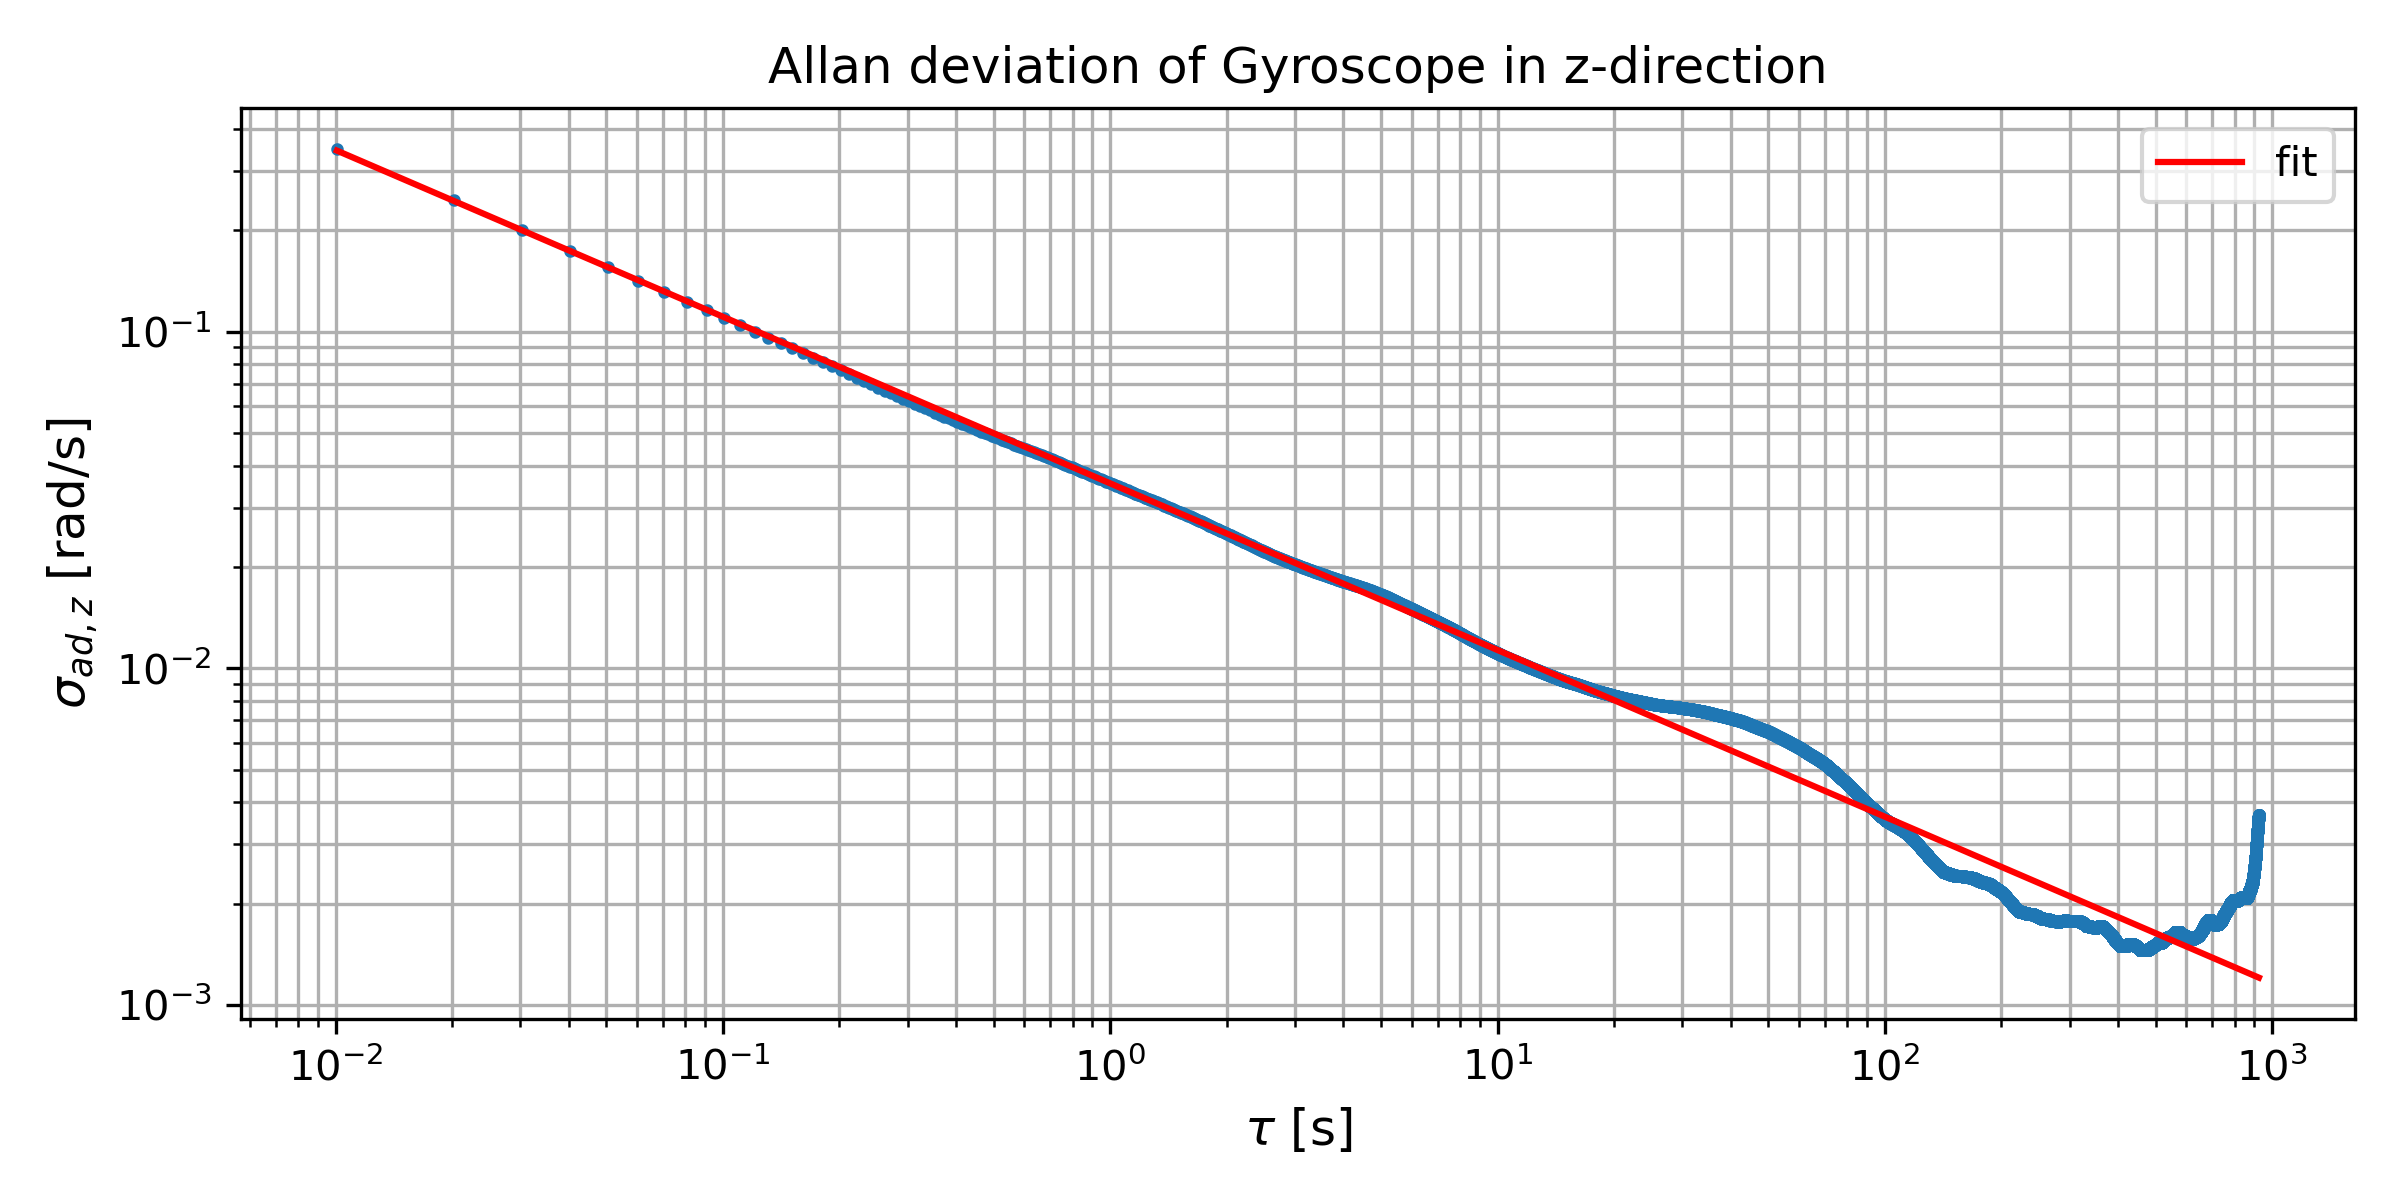
\includegraphics[width=0.7\columnwidth]{prelab_allan_z.png}}}

	\caption{The Allan deviation for each gyroscopic component for each integration time $\tau$. The log-linear fit is 
	also shown.}
	\label{fig:prelab_allan}
\end{figure*}


The shot-noise time interval, which is the integration time up until the point where the instability of the instrument or drift dominates, 
can be determined as the point where the first minima of the plot is observed. From Fig. \ref{fig:prelab_allan}, we observe that the
point of instability of the x direction occurs at a much earlier integration time than compared to those from the y and z directions. 
This indicates that the bias from the x direction affected the Allan deviation measurement. \par 

We also determine the shot-noise limited sensitivity $\mathcal{A}$ 
by performing a log-linear fit according to Eq. \ref{eq:allan_shotnoise}. 
By taking the logarithm on both sides, we obtain an equation that can be linearized as such:
\begin{equation}
	\log(\sigma_{\mathrm{ad}}) = m \log(\tau) + \log \mathcal{A}
\end{equation}
where $m$ should yield $-0.5$ due to the shot-noise scaling. The shot-noise limited sensitivity can then be obtained
by taking the exponential of the intercept from the log-linear fit. The data was truncated after the point of instability for 
each direction. Fig. \ref{fig:prelab_allan} shows the log-linear fit for each component. Table \ref{tab:prelab_allan_vals} show the shot-noise limited time interval and the fit parameters (the slope $m$ and the shot-noise 
limited sensitivity $\mathcal{A}$) for each component. 

\begin{table}[h!]
	\centering
	\begin{tabular}{|c|c|c|c|c|}
		\hline 
		Component & $\tau$ [$\si{\second}$] & $m$ & $\mathcal{A}$ [\si[]{\radian\per\second\per\sqrt{\hertz}}] & $|m - (-0.5)|$\\ \hline
		x & 1 & -0.3925 & 0.0576  & 0.1106\\ \hline
		y & 10 & -0.4318 & 0.0395 & 0.0677\\ \hline
		z & 20 & -0.4952 & 0.0354 & 0.0048\\ \hline
	\end{tabular}
	\caption{The shot-noise limited time interval and associated fit parameters from the log-linear fit of the Allan deviation
			in each component. \hl{Fix table width}}
	\label{tab:prelab_allan_vals}
\end{table}

We observe that the time intervals vary between each component, however $\tau_x$ is one order of magnitude smaller than those from 
the y and z direction. This indicates that the bias observed in Fig. \ref{fig:prelab_allan_fourier} influenced the measurement of the 
Allan deviation. \par 

When comparing the fit parameters, we observe that the slope from the z component yield the value most closest to $-0.5$, which may be 
due to the longer shot-noise time interval, which in turn allows more data points to be fit. However, all components yield slopes
close to $-0.5$, with the largest deviation from the x-direction with a residual of $\sim 0.11$. We also observe that the shot-noise
limited sensitivity from the x component is approximately $0.02$ larger than that of the y and z components. This again 
indicates the influence of the bias of measurement in the x direction. This also shows that the phone's gyroscope is more sensitive
to measurements in the y and z direction as compared to that of the x direction. 

\section{Task 3: Rotation Rate of Earth}

To determine the rotation rate of the Earth, we utilize the same method as we have performed to measure the Allan deviation, but we 
perform this for the shot-time limited interval derived by the section above. \par 

We first measure the gyroscope $x, y, z$ coordinates for the duration of the shot-time interval of $\tau = 700$s. After the data was recorded,
we performed the same measurement but with the phone flipped upside down. This corresponds to a flip in the $y$ direction. 
We then performed the same process but flipping in the $z$-direction instead (i.e. rotations parallel to the surface). This was performed for a 
shorter duration of $\tau = 300$s due to time constraints. The corresponding time series for both results are shown in Fig. \ref{fig:raw_earth_y_faceup}, \ref{fig:raw_earth_y_facedown}, \ref{fig:raw_earth_z_faceup} and \ref{fig:raw_earth_z_facedown}.


\begin{figure}[hbt!]
     \centering
	 {{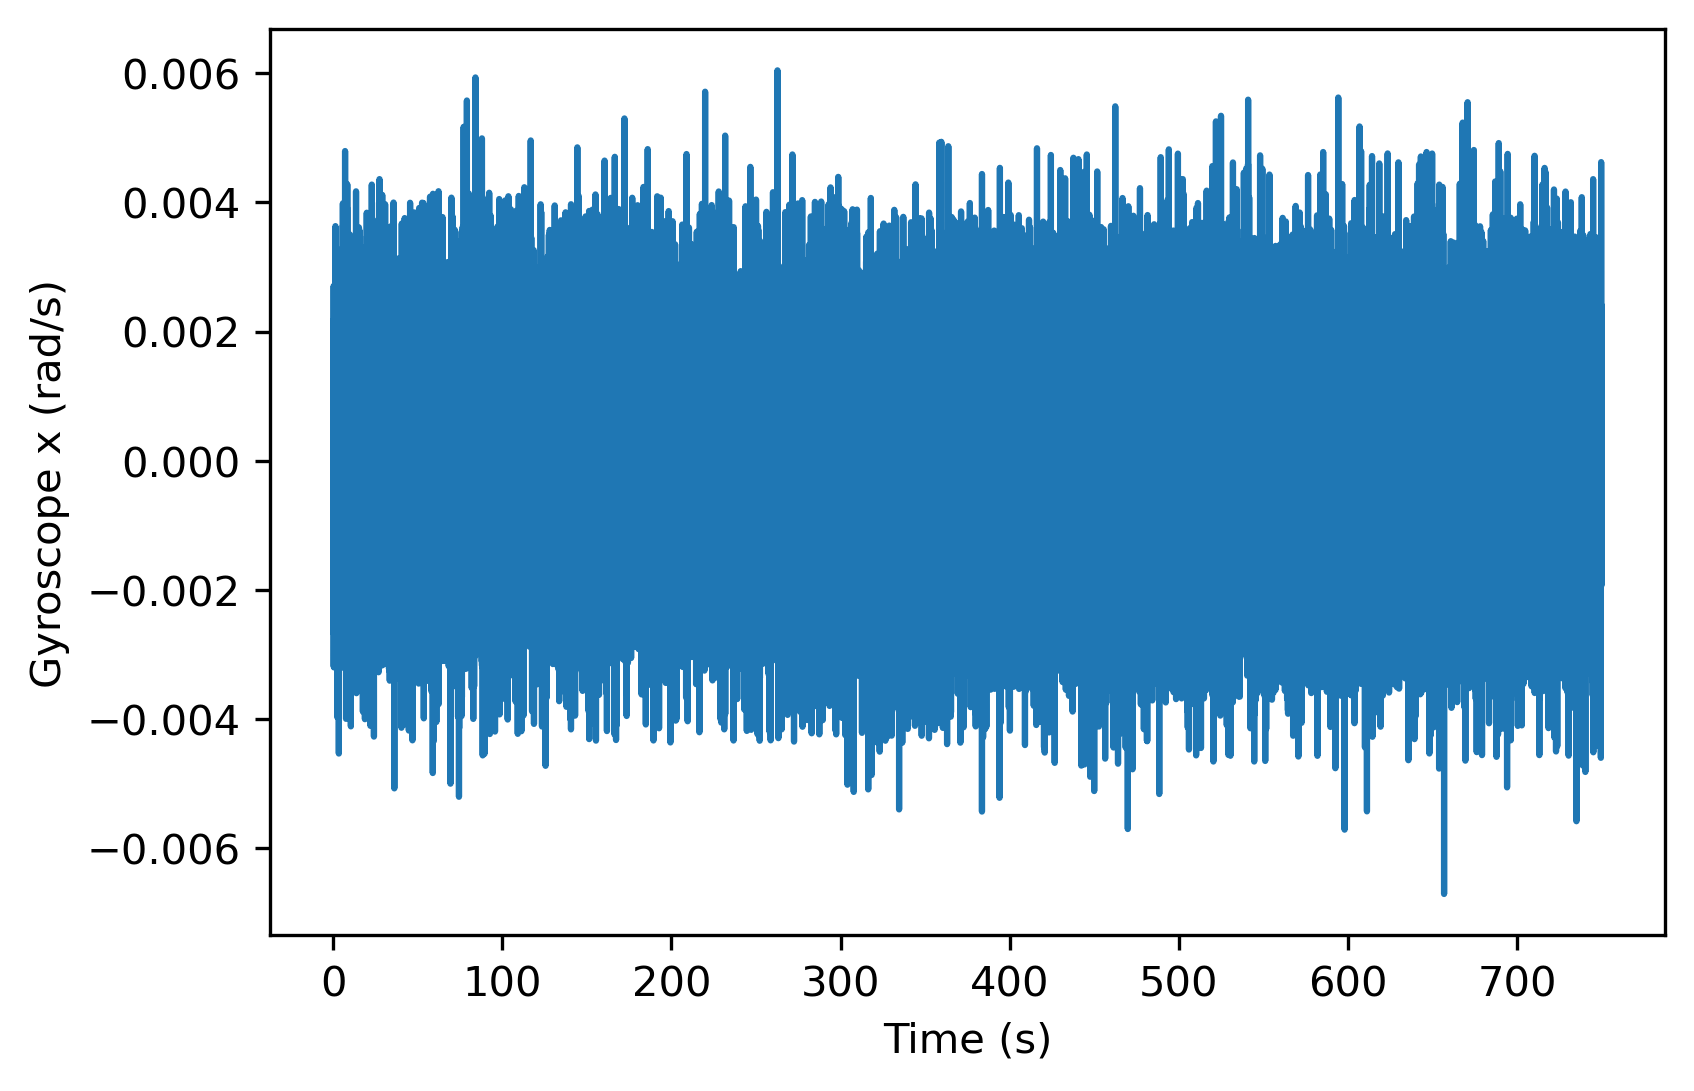
\includegraphics[width=0.4\columnwidth]{raw_ftx.png}}}
	 {{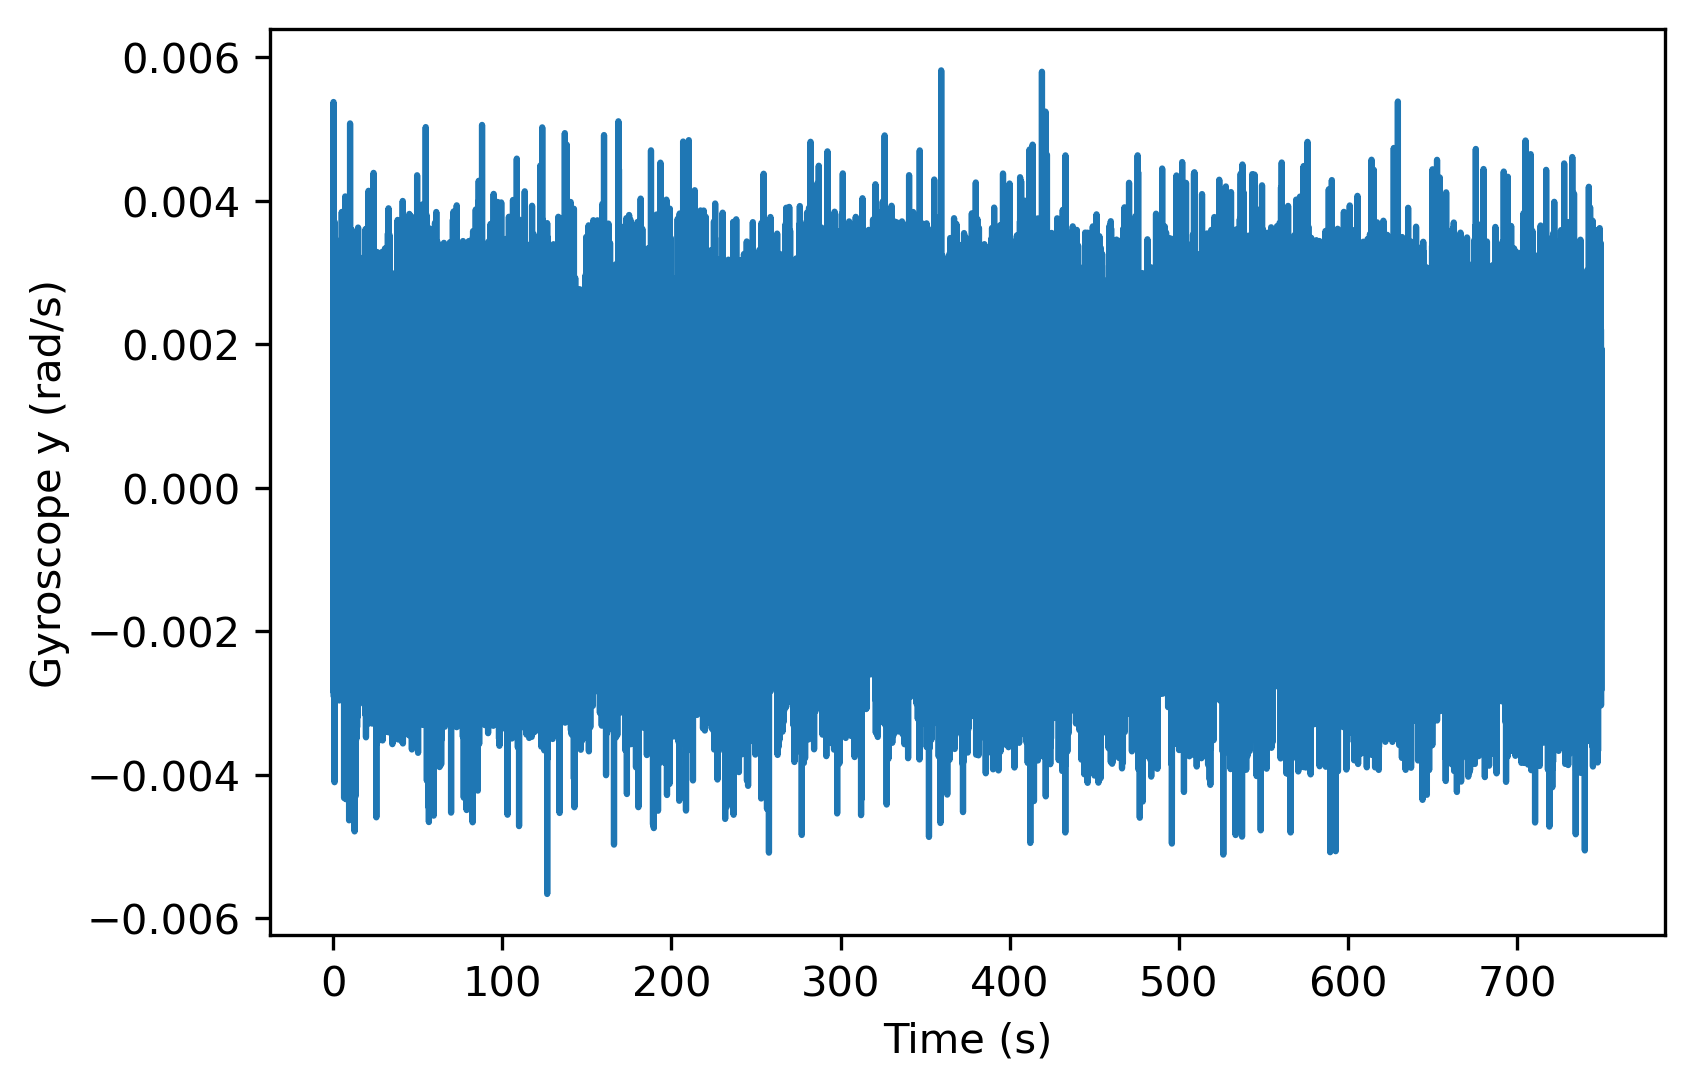
\includegraphics[width=0.4\columnwidth]{raw_fty.png}}}
	 {{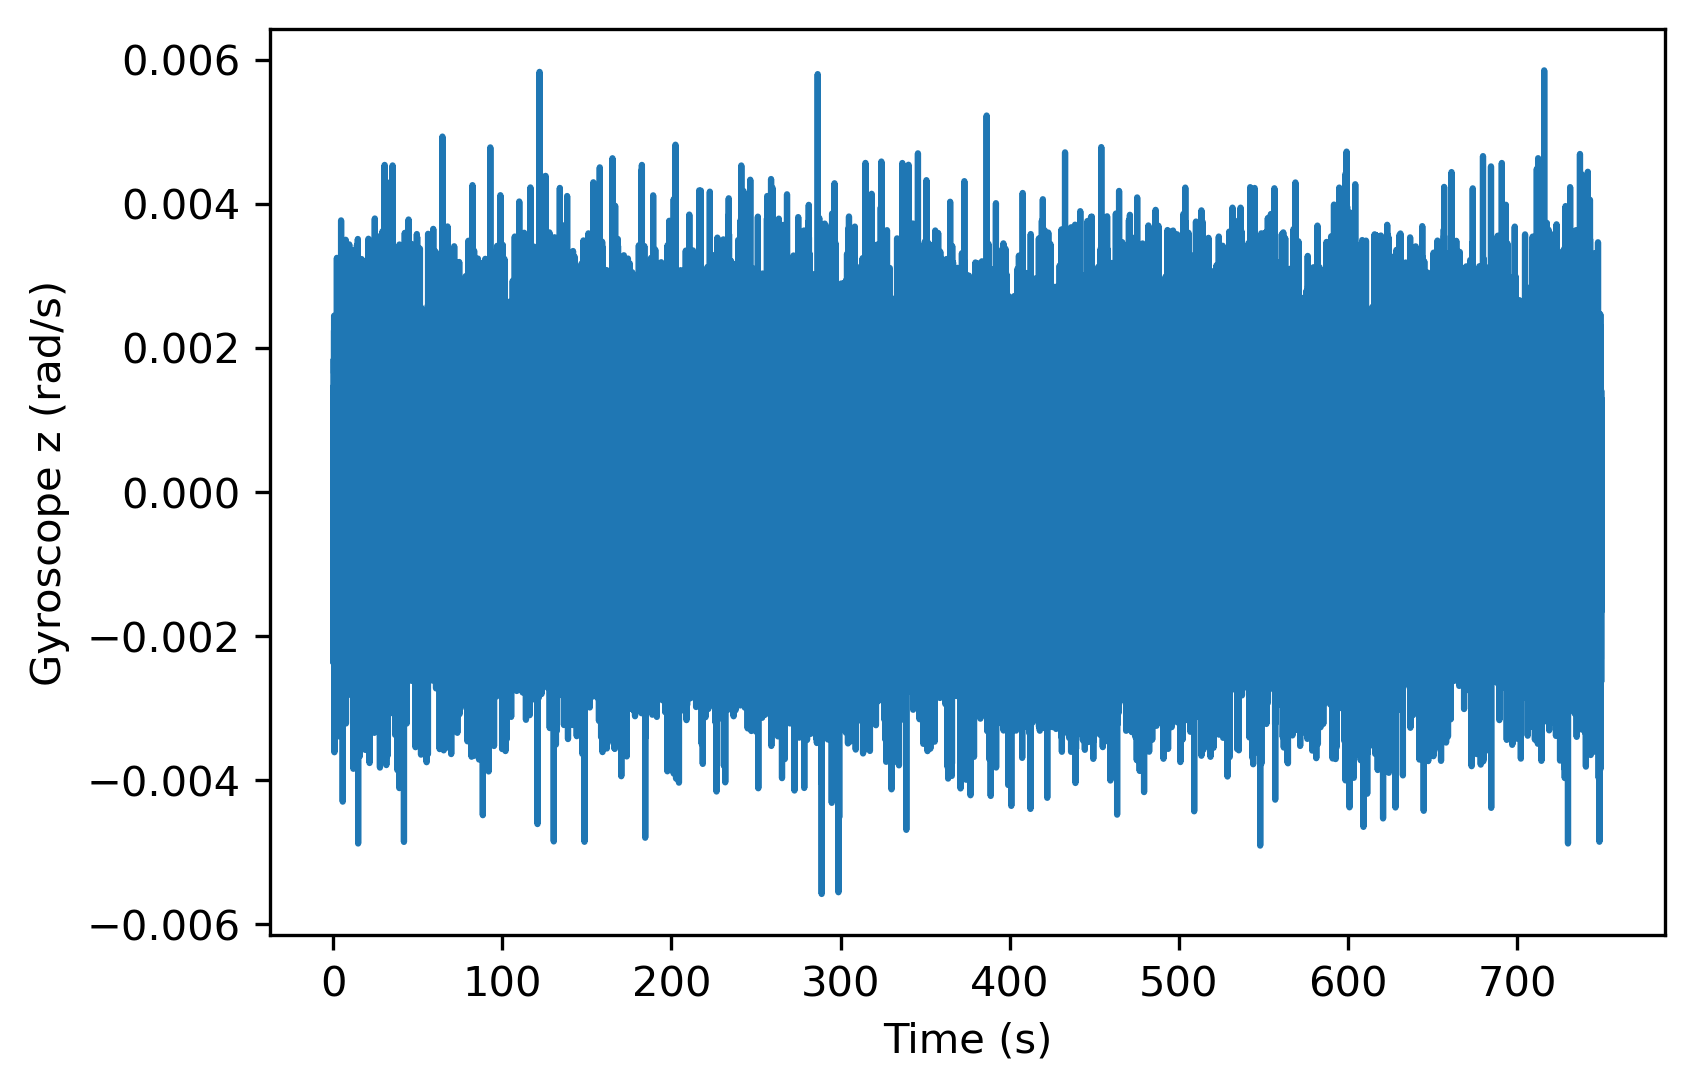
\includegraphics[width=0.4\columnwidth]{raw_ftz.png}}}

     \caption{Raw data of all the three axes of gyroscope from phone for measurement of the Earth's rotation.
               The measurement was took with the phone face up. }
	 \label{fig:raw_earth_y_faceup}
\end{figure}

\begin{figure}[hbt!]
     \centering
     {{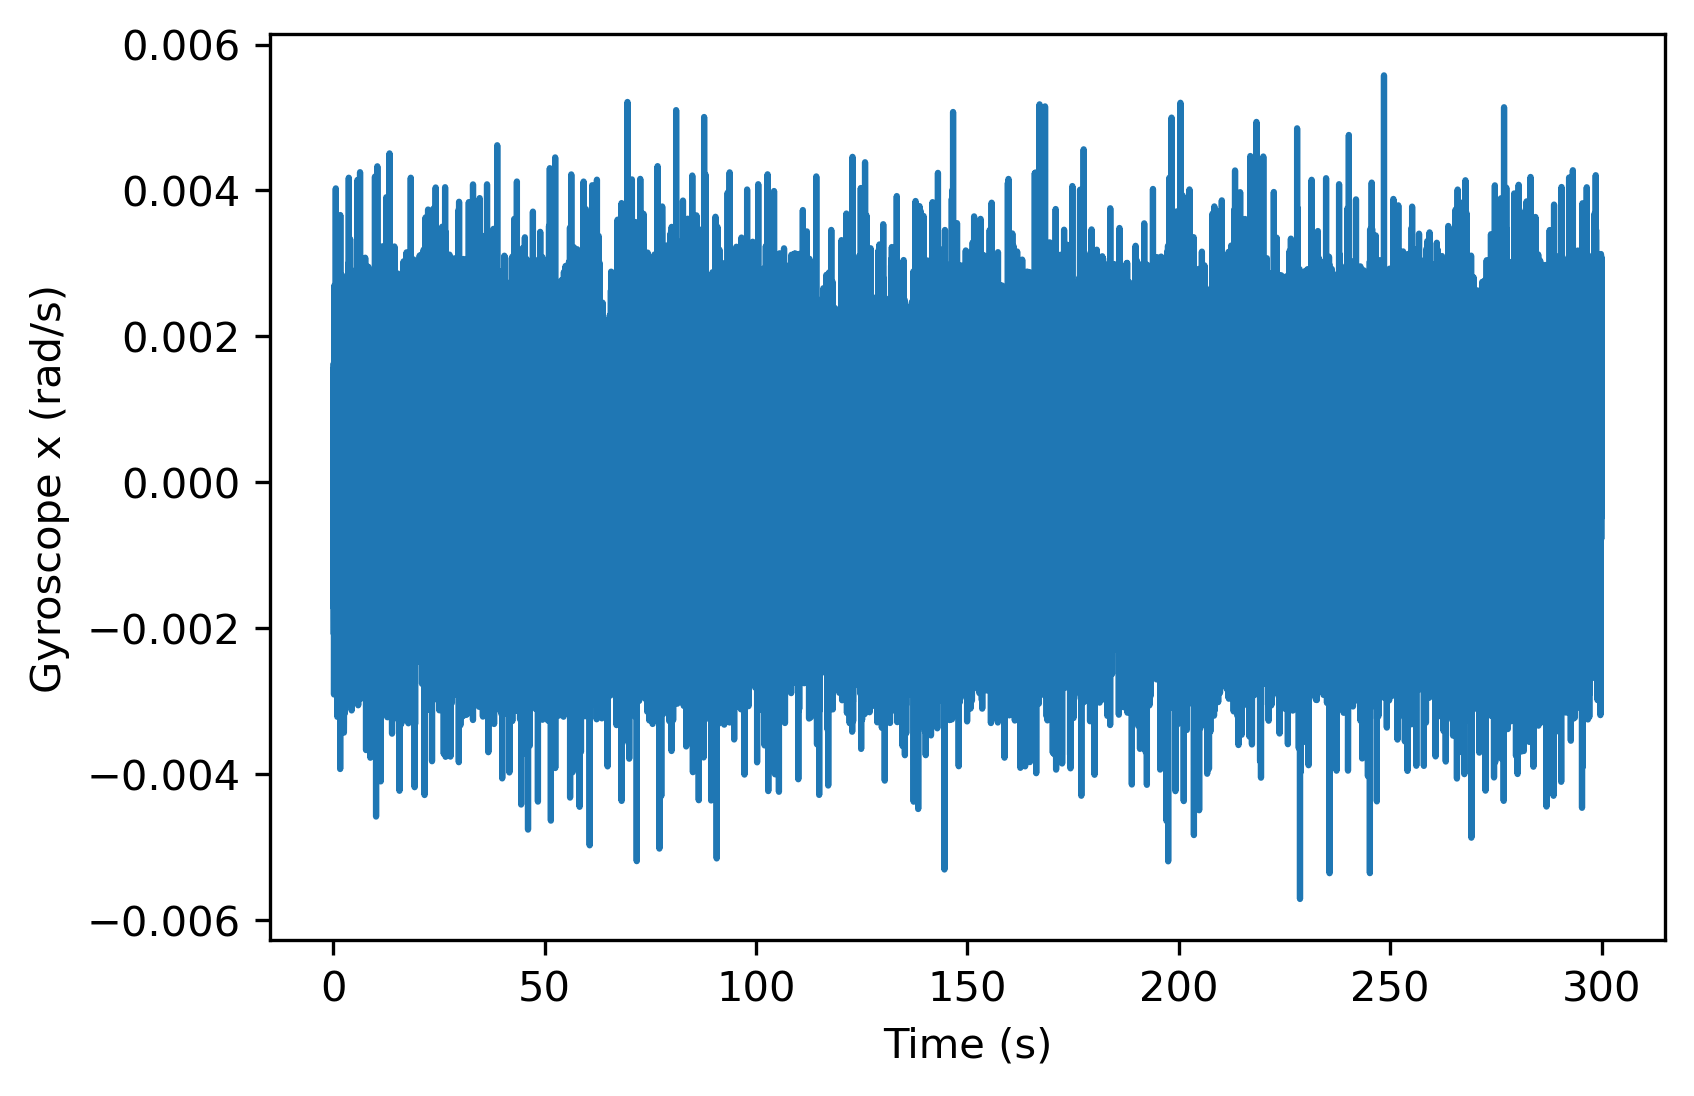
\includegraphics[width=0.4\columnwidth]{raw_btx.png}}}
     {{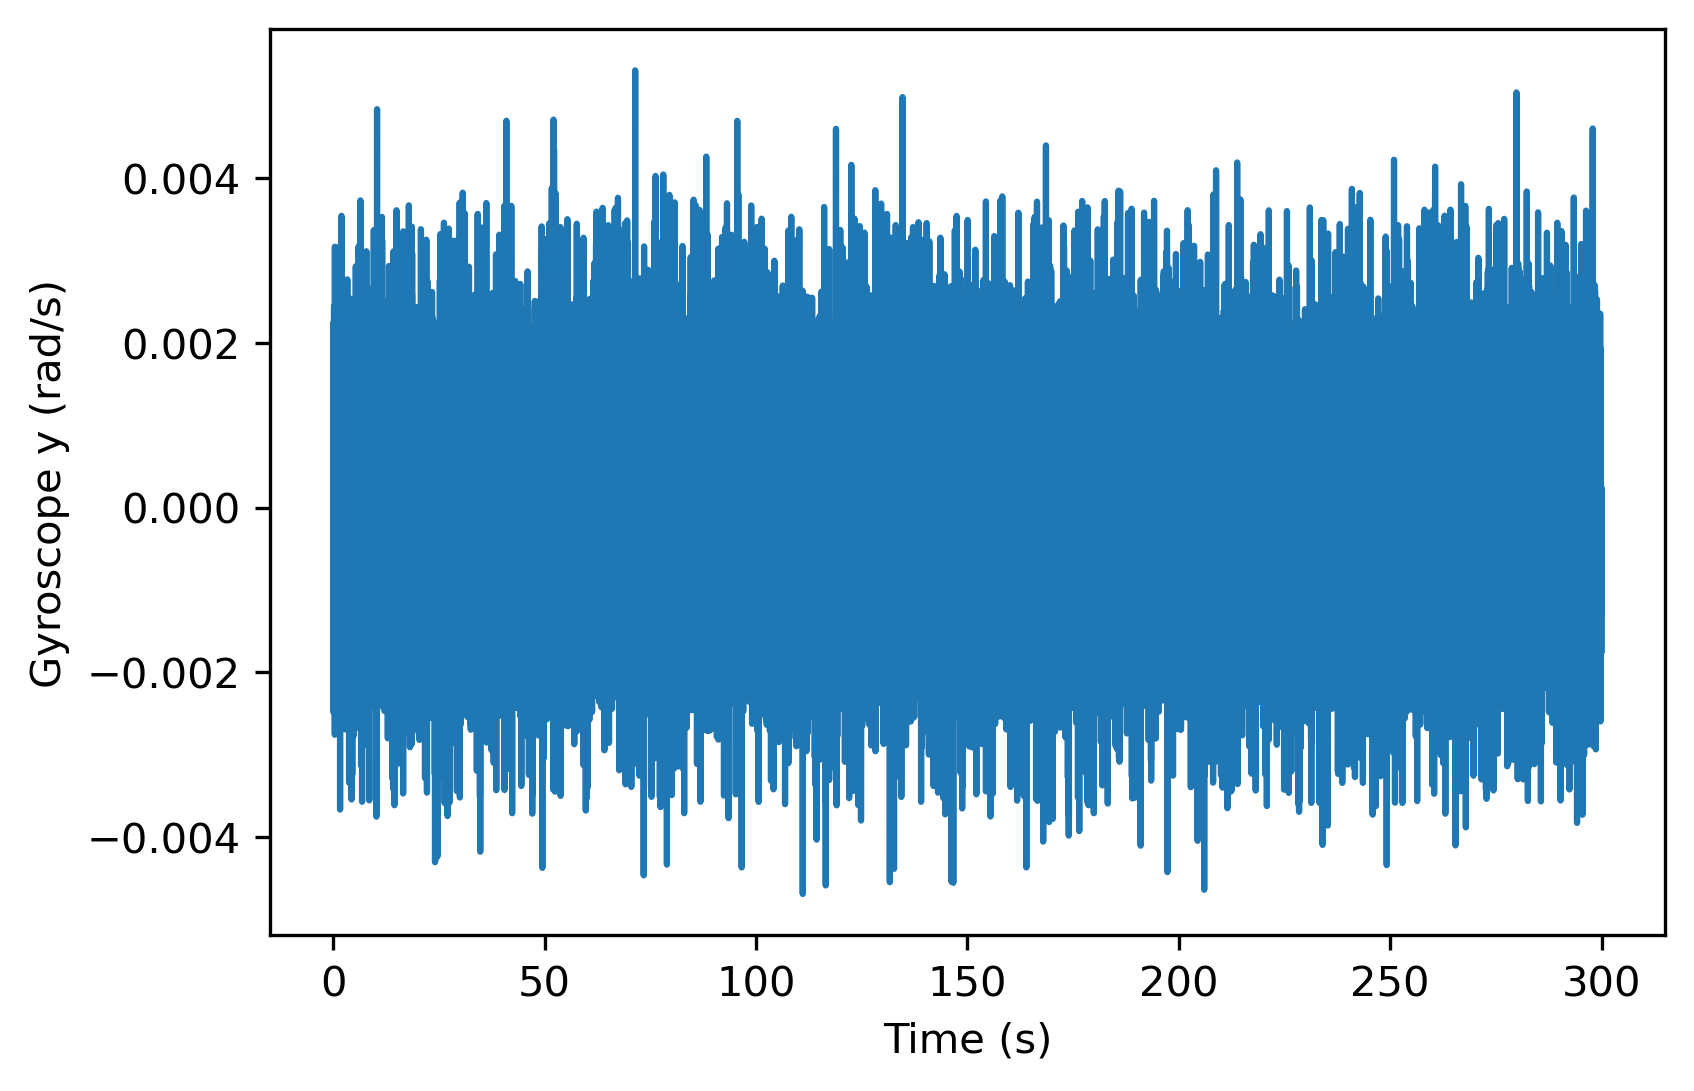
\includegraphics[width=0.4\columnwidth]{raw_bty.png}}}
     {{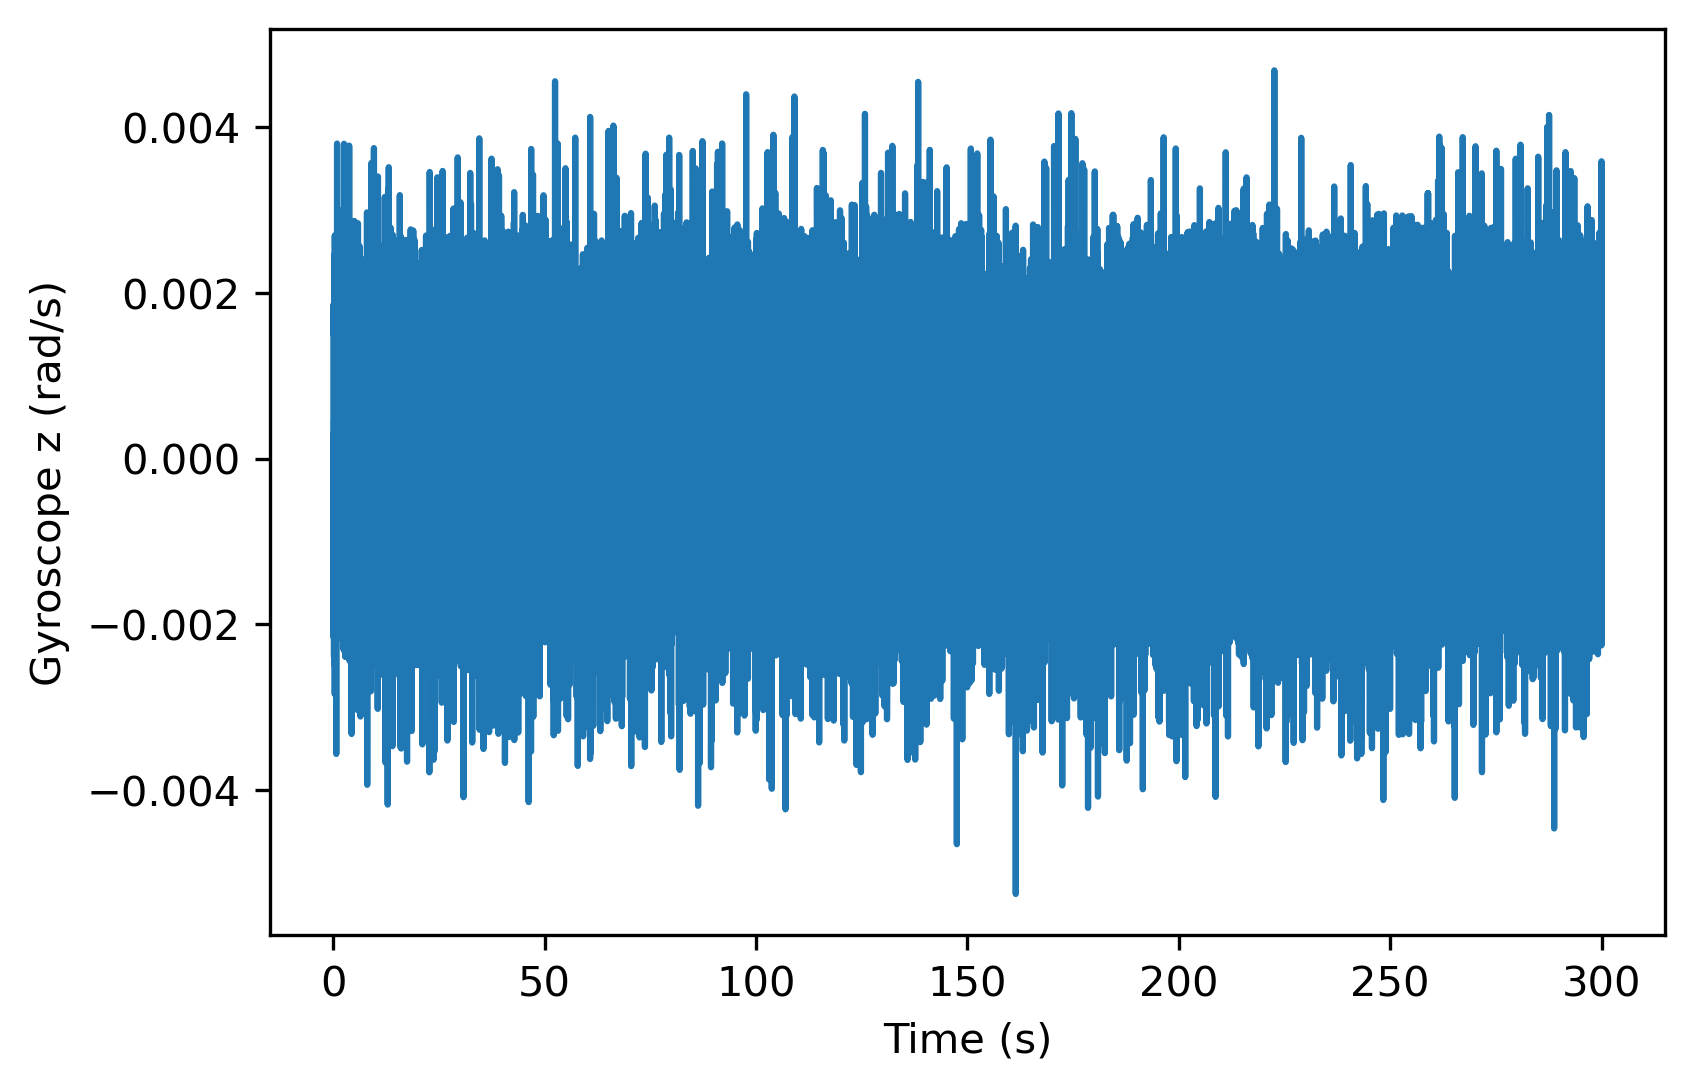
\includegraphics[width=0.4\columnwidth]{raw_btz.png}}}
     \caption{Same as Fig. \ref{fig:raw_earth_y_faceup} but for phone face down instead.}
     \label{fig:raw_earth_y_facedown}
\end{figure}

\begin{figure}[hbt!]
     \centering
	 {{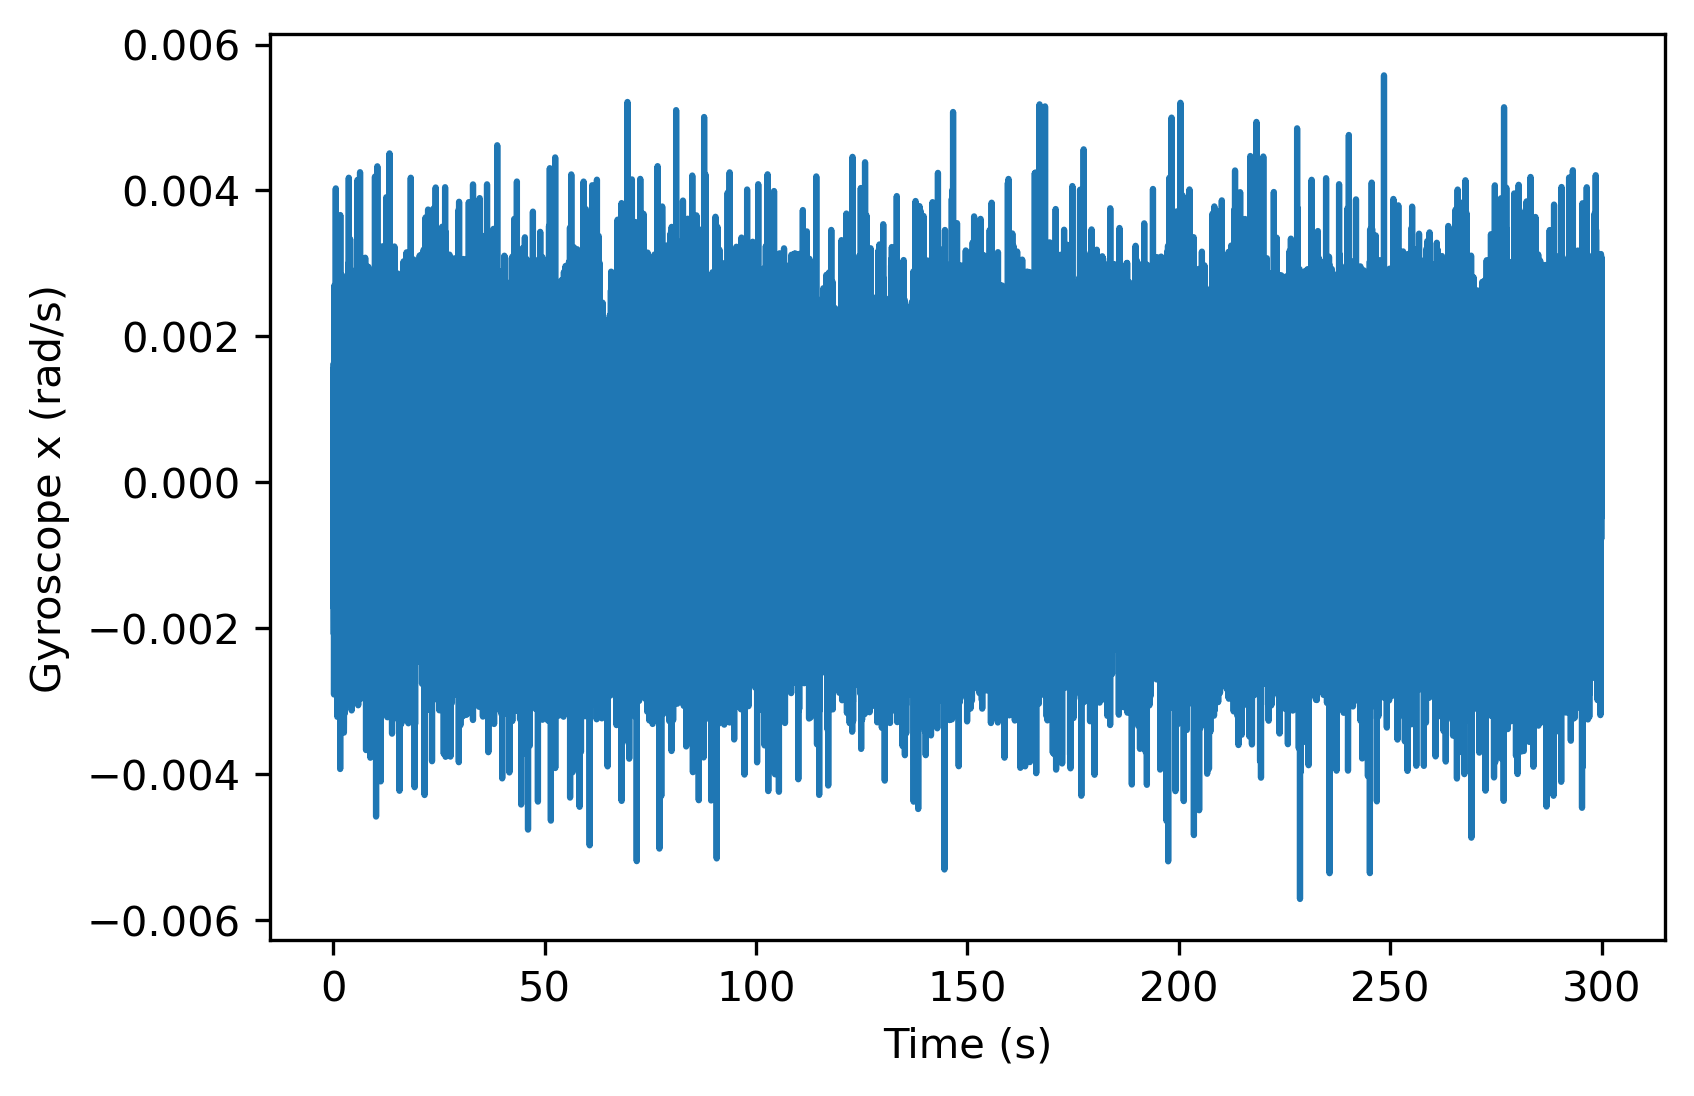
\includegraphics[width=0.4\columnwidth]{raw_okx.png}}}
	 {{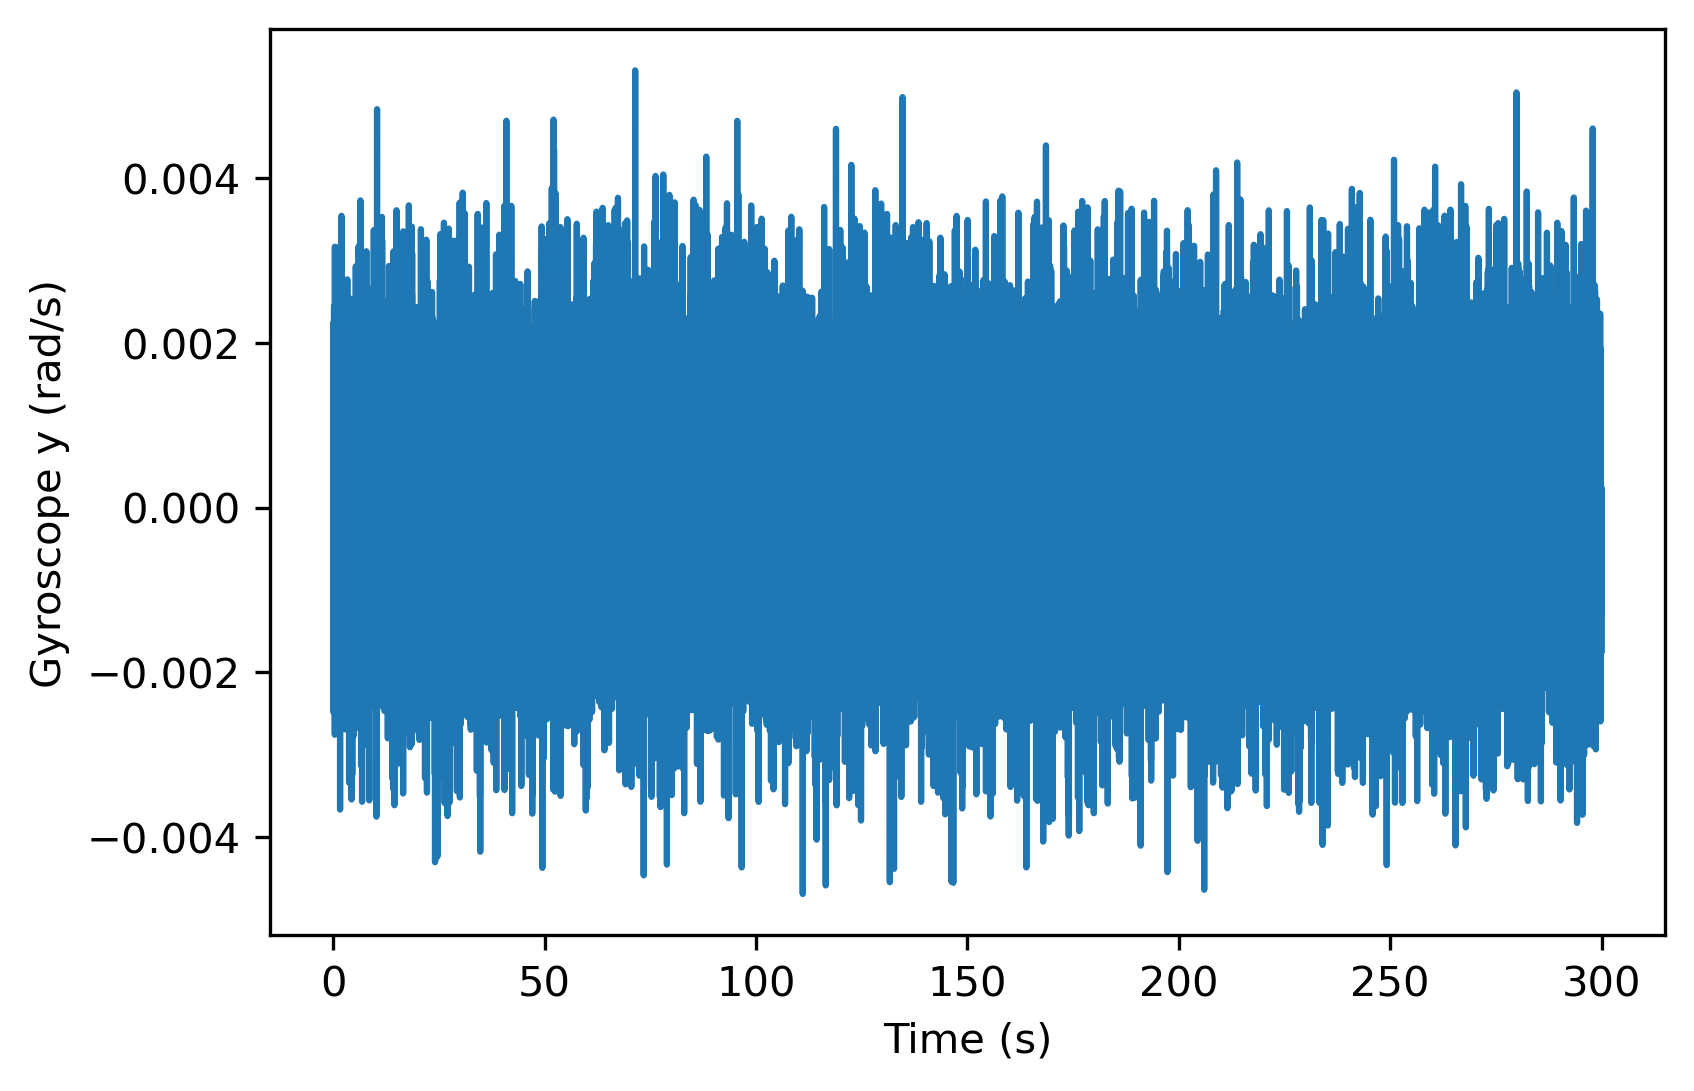
\includegraphics[width=0.4\columnwidth]{raw_oky.png}}}
	 {{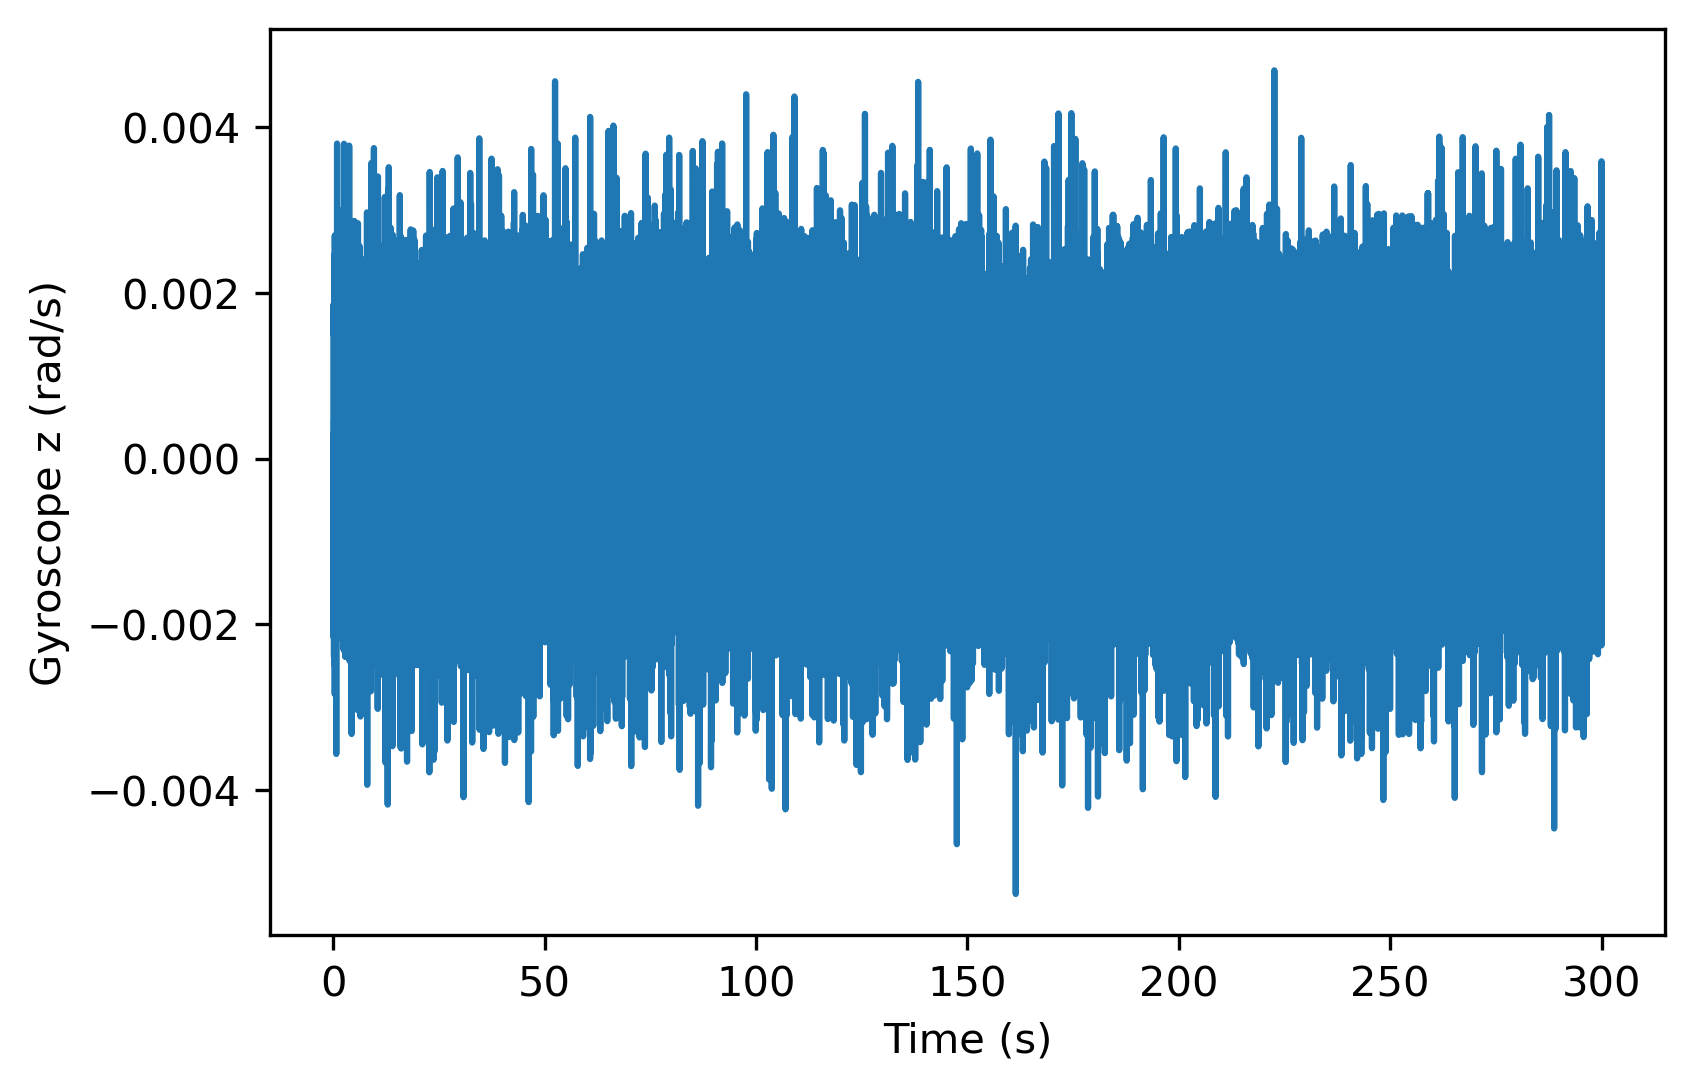
\includegraphics[width=0.4\columnwidth]{raw_okz.png}}}

     \caption{Same as Fig. \ref{fig:raw_earth_y_faceup} but for rotations in the $z$-direction. This was performed 
               with the phone facing towards the South Pole. }
	 \label{fig:raw_earth_z_faceup}
\end{figure}

\begin{figure}[hbt!]
     \centering
     {{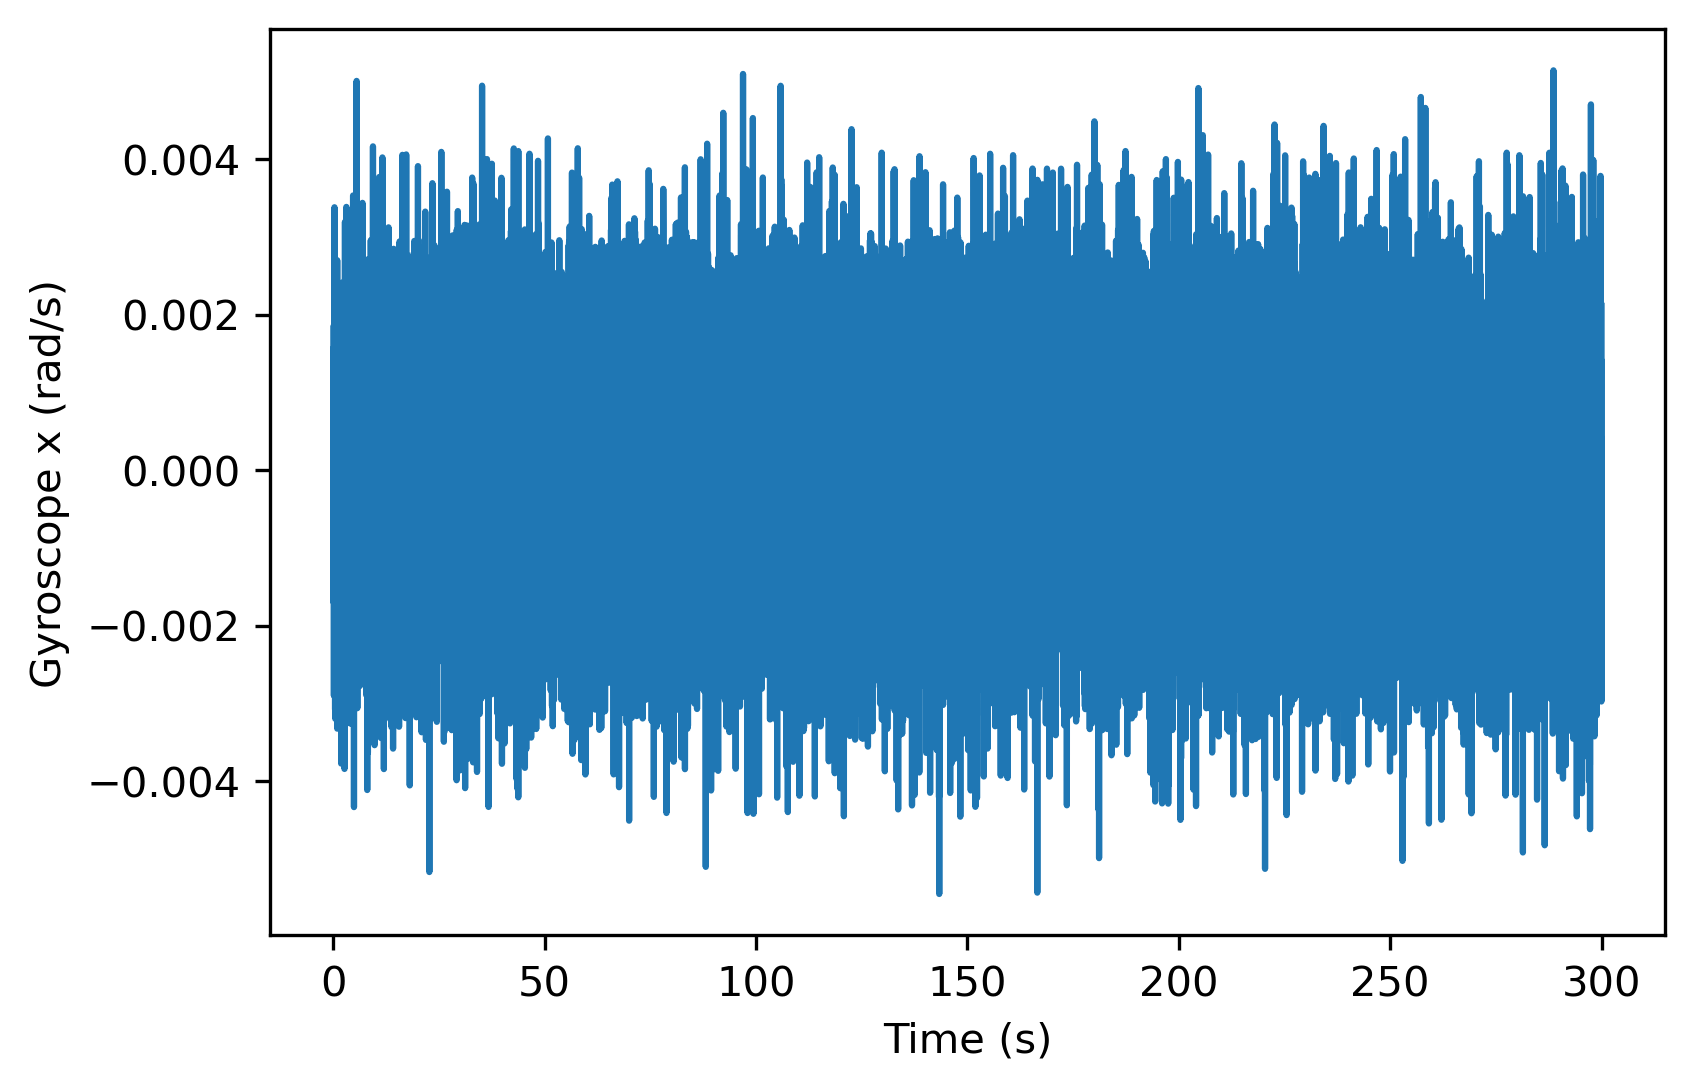
\includegraphics[width=0.4\columnwidth]{raw_180kx.png}}}
     {{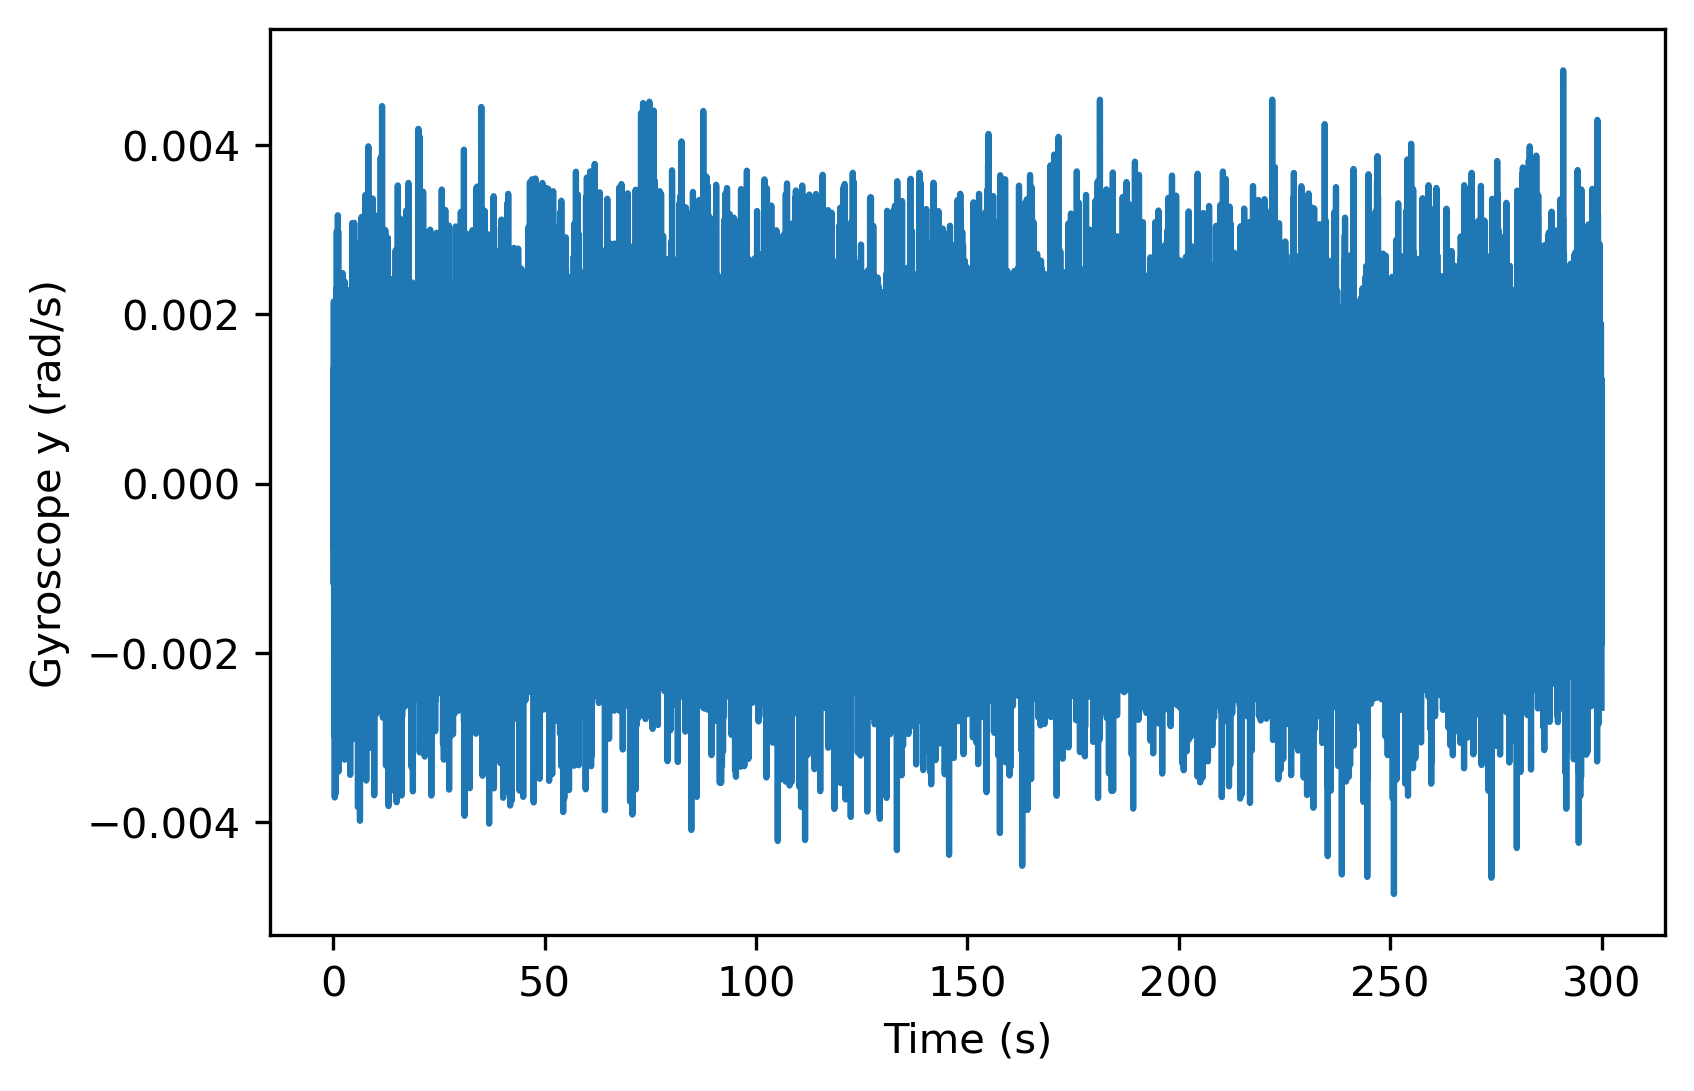
\includegraphics[width=0.4\columnwidth]{raw_180ky.png}}}
     {{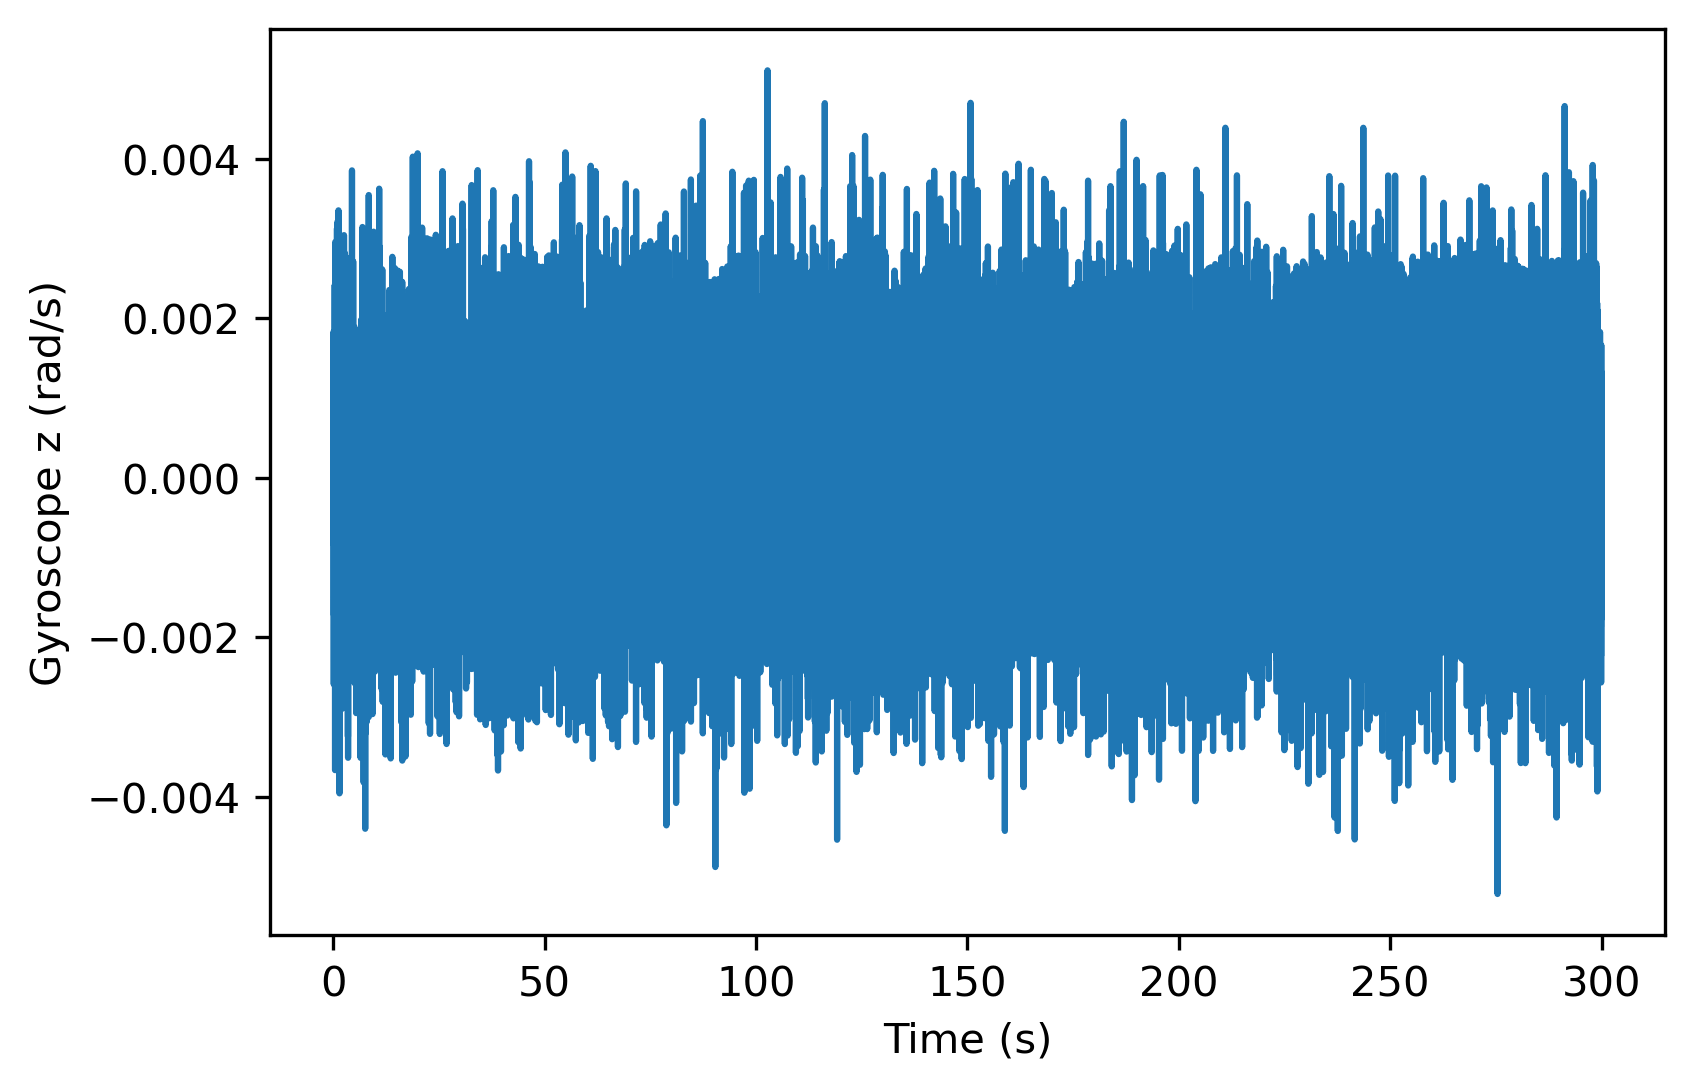
\includegraphics[width=0.4\columnwidth]{raw_180kz.png}}}
     \caption{Same as Fig. \ref{fig:raw_earth_z_faceup} but for those facing towards the North Pole instead.}
     \label{fig:raw_earth_z_facedown}
\end{figure}


After performing the FFT onto the resulting time series, we observed the sharp peak in the gyroscope $x$-direction.
This shows that there is a clear bias in the $x$-direction of the phone gyroscope. 

The temporal average of each measurement (both flipped and unflipped) was taken, and the difference between the unflipped and flipped
measurements were taken (normalized by 2). For example, for the $x$ coordinate we have: 
\begin{equation}
     \delta \bar{\omega_x} = \frac{|\bar{x}_{noflip} - \bar{x}_{flip}|}{2}
\end{equation}

Such measurements for both rotations are tabulated on Table \ref{tab:avg_rate_xyz}. The magnitude of the values are also evaluated.
Note that for arbitrarily small differences, the deviations may be small and thus to properly normalize this, one needs to take
into arround the uncertainty in the measurement as well. 

\begin{table}
\centering
\begin{tabular} {|c|c|c|}
 \hline
 Coordinate & $\delta \bar{\omega_i}$, face up/down (rad/s) & $\delta \bar{\omega_i}$, face North/South (rad/s) \\
 \hline
 $x$ & $\num{9.273e-8}$ & $\num{9.956e-6}$ \\
 \hline
 $y$  & $\num{4.603e-7}$ & $\num{2.814e-5}$ \\
 \hline
 $z$ & $\num{2.340e-6}$ & $\num{3.357e-6}$  \\
 \hline
 $\omega$ & $\num{2.386e-6}$ & $\num{3.004e-5}$ \\
 \hline
\end{tabular}
\caption{Difference of temporal average of rotation rate for each gyroscopic coordinate and its magnitude. }
\label{tab:avg_rate_xyz}
\end{table}
 
Furthermore, to properly account for the Earth's rotation rate, we need to transform from the local frame in which we observe the phone's orientation in.
This can be done by a simple coordinate transformation as such: $\omega = \Omega_E \cos\phi$, where $\phi$ is the geographic latitude.
With $\phi = \SI{39.257}{\degree}$ (defined from the North Pole), we obtain our corrected rotation rate of the Earth as 
$\Omega_E = 3.083\mu \text{rad}s^{-1}$ and $\Omega_E = 38.80\mu \text{rad}s^{-1}$ for the up/down and North/South
flip case respectively.  \par 

When comparing the values of the rotation rate to the analytical value $\Omega_{E, thr} = 72.92\mu \text{rad}s^{-1}$, 
both yielded values are underestimated. However, the rate where the phone was flipped upside down yielded lower values
compared to that when we flipped the phone from South to North. This indicates a clear bias in the rotation and how it 
impacts the measurement, which is clear due to the East-West rotation of the Earth. \par 

Furthermore, the underestimation of the values are clear due to the various systematical uncertainties that need to be accounted for.
The movement of nearby people, the wind, the temperature differences can all impact the phone gyroscope in some way. The 
MEMS gyroscope does not have as many tools that will calibrate for such deviations as compared to our experimental setup. 


\chapter{Experimental Set-Up and Procedure}

\section{Experimental Set-Up}

In this experiment, we use a interference filter laser diode with $\lambda = \SI[]{1064}[]{\nano\metre}$ as our laser, placed 
outside of the ring cavity system. The signal is then transmitted through an electro-optical phase modulator (EOM). The EOM 
generates sidebands of $\Omega / (2\pi) = \SI{10}{\mega\hertz}$. Each beam is then passed through an acousto-optical modulator (AOM),
where the light is diffracted with a frequency of approximate;y $\SI[]{200}[]{\mega\hertz}$. The beams are then passed through 
a square cavity with an arm length of approximately $\SI[]{0.25}[]{\centi\metre}$, placed on a rotating table. The cavity consists of four mirrors with high
reflectivity, and allows the laser to be passed through the cavity in a clockwise or counter-clockwise manner. A plexiglass covering
is placed around the cavity to limit any degradation of the reflectivity due to dust \cite{Groh2021}. 
Fig. \ref{fig:exp_setup} shows the setup of the experiment, and Fig. \ref{fig:exp_schematic} shows the schematic of the set-up.

\begin{figure*}[h!]
	\centering
	\includegraphics[width=0.6\columnwidth]{exp_setup_picture.png}
	\caption{The set-up used in this experiment.}
	\label{fig:exp_setup}
\end{figure*}

\begin{figure*}[h!]
	\centering
	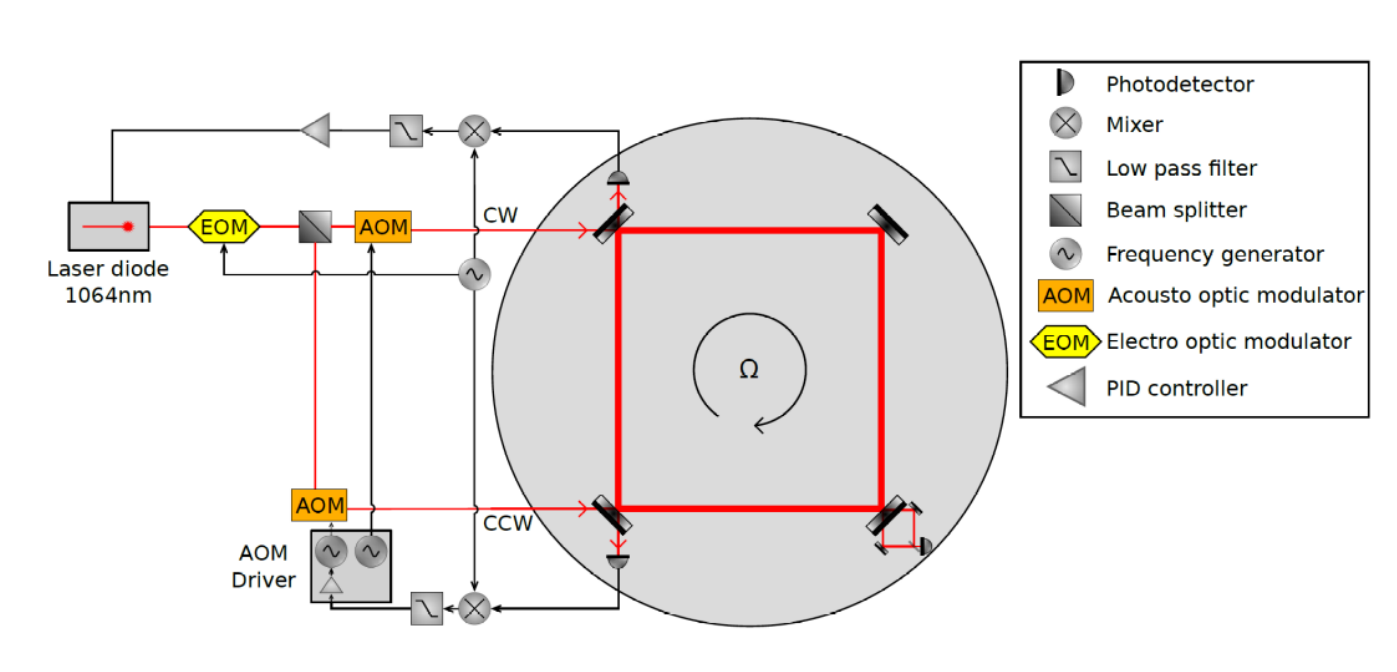
\includegraphics[width=0.8\columnwidth]{setup_schematic.png}
	\caption{The schematic of the set-up. Obtained from Ref. \cite{Groh2021}.}
	\label{fig:exp_schematic}
\end{figure*}

In order to perform the laser locking, the signal from the cavity is passed into the Moglabs laser lock box, in which the fast and slow PID 
controller controlled the laser frequency. For PID optimization, we configured the parameters given in the laser lock box
until the lock was stable with a high intensity. To lock the laser, we turned the two switches located next to the parameter controls
simultaneously. To observe the corresponding signal from the first laser, we connected the drivers to an oscilloscope. This setup was used 
to determine the free spectral range and the PDH error signal \cite{Groh2021}. The obtained signal was exported through a \texttt{.csv} file
via a USB port. Fig. \ref{fig:exp_setup_devices} show the oscilloscope, Moglabs laser lock box, 
and EOM used in this experiment.\par 

\begin{figure*}[h!]
	\centering
	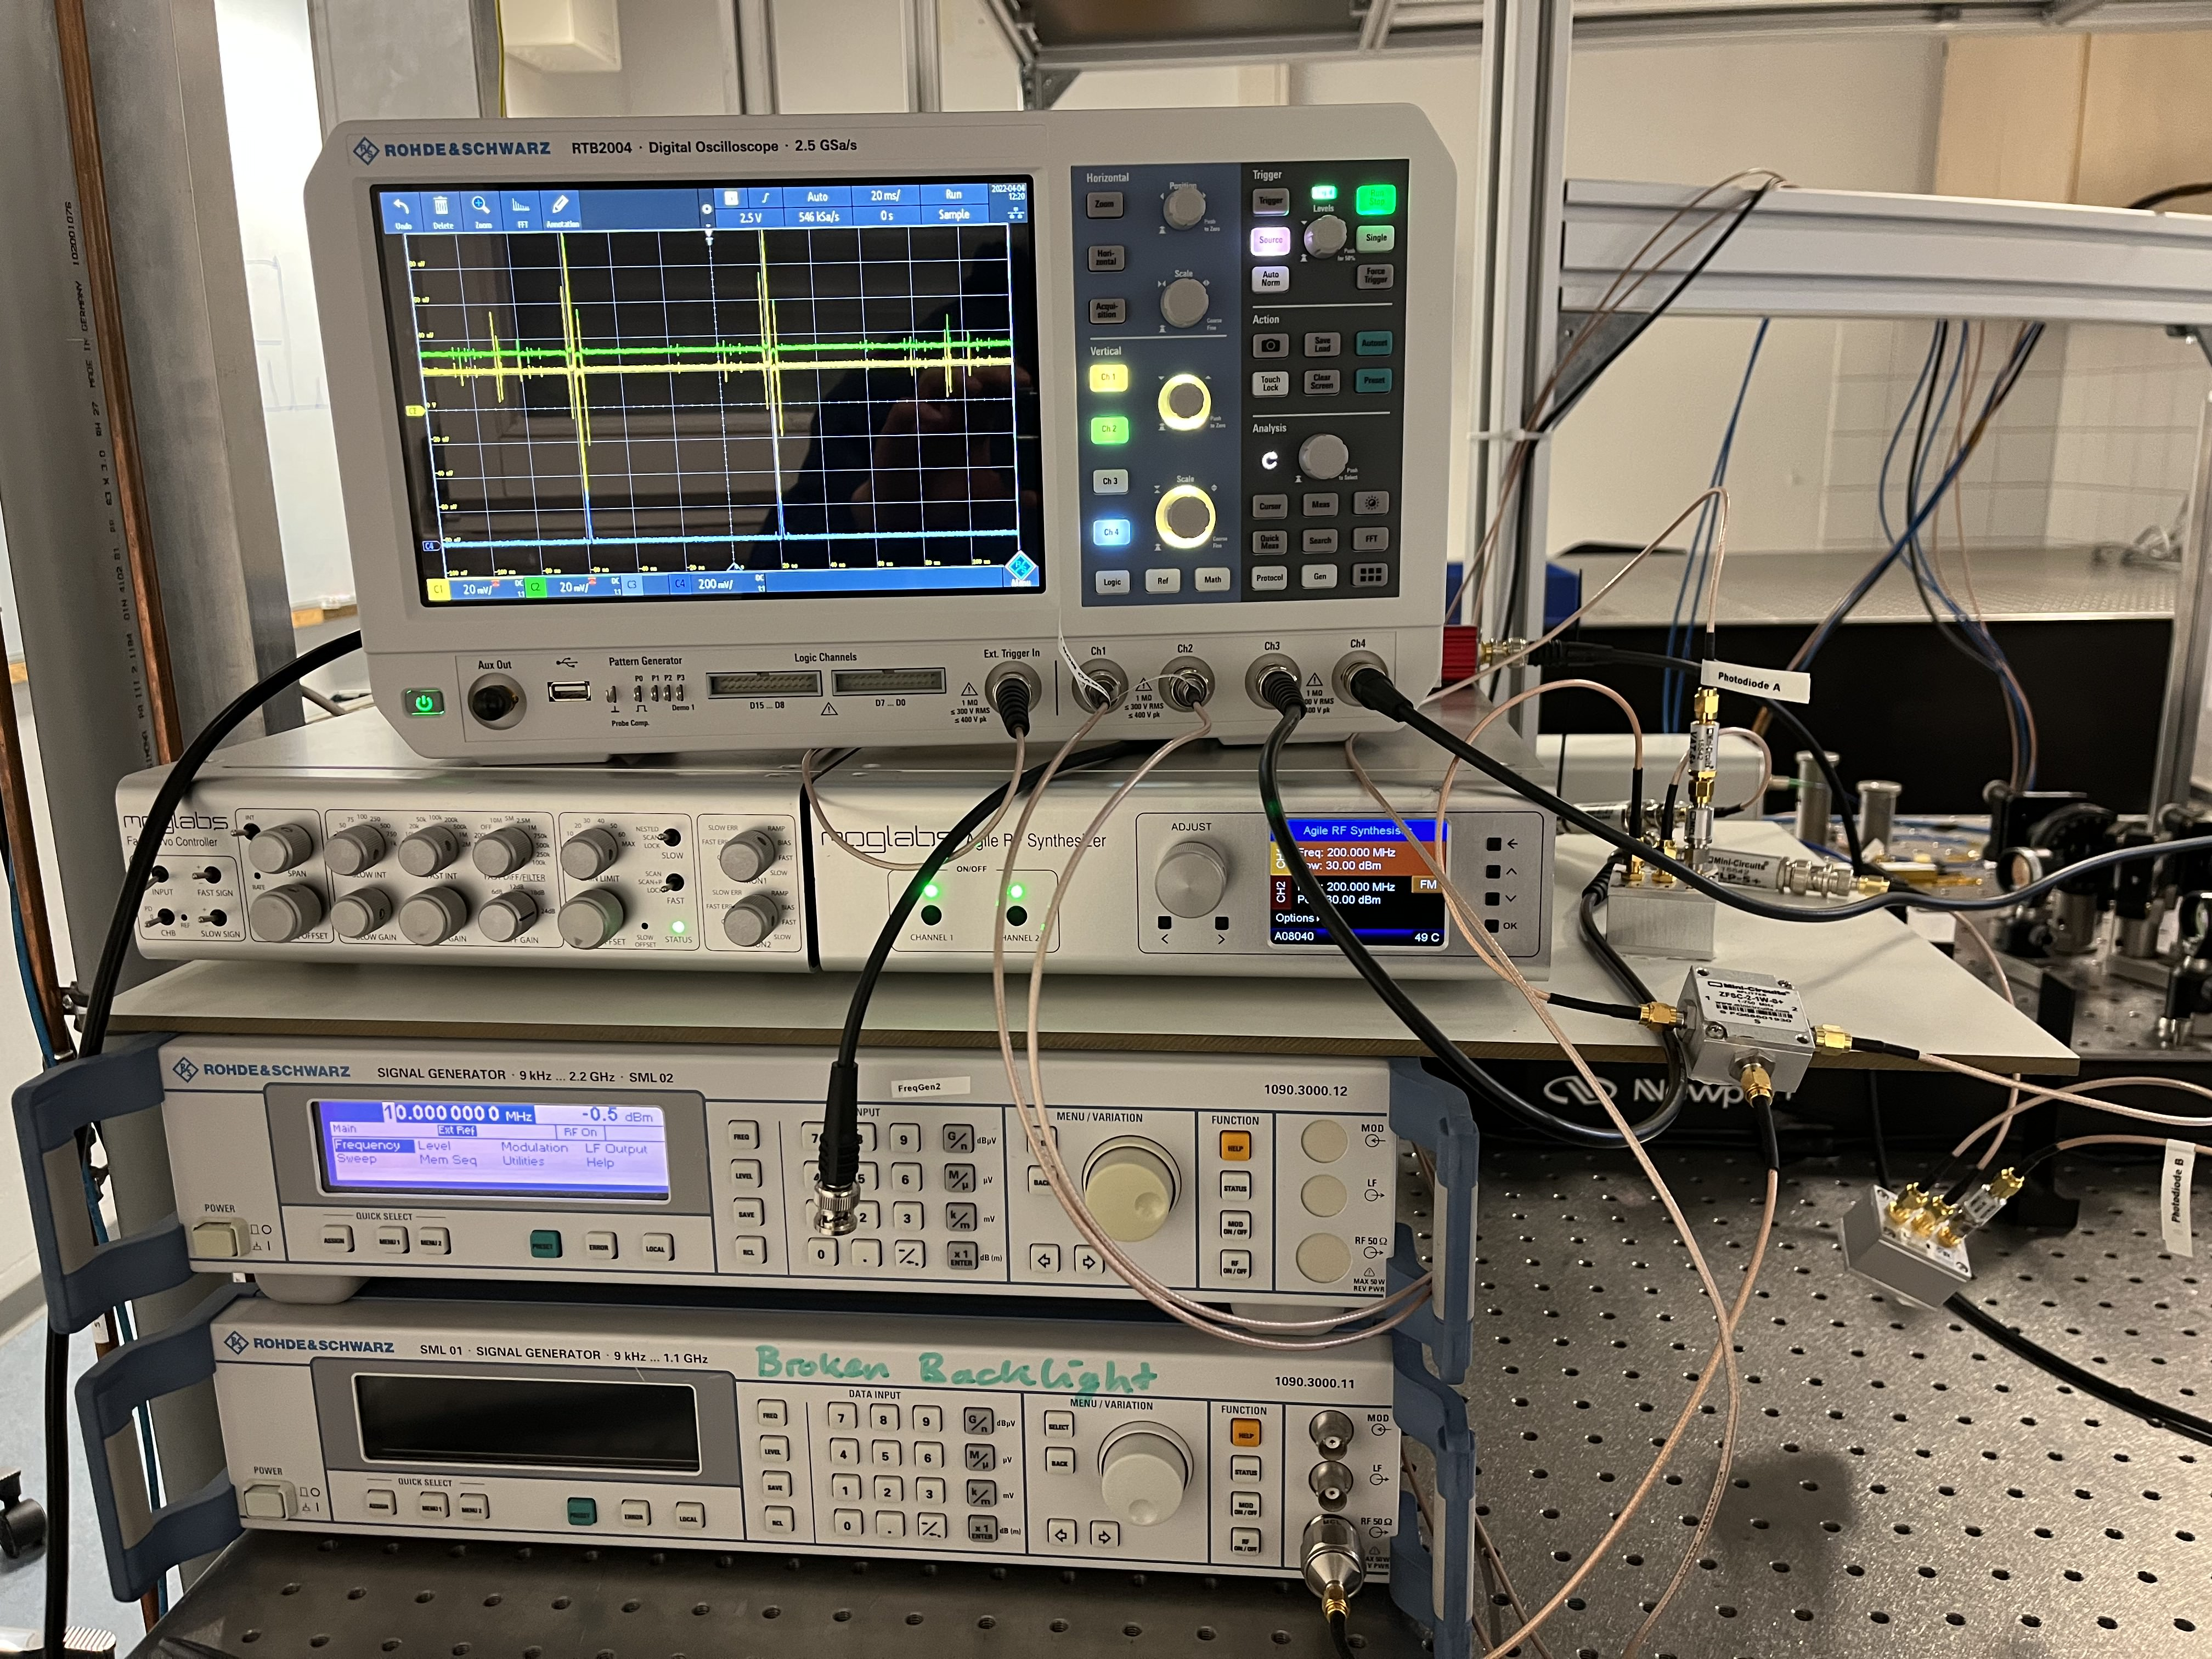
\includegraphics[width=0.8\columnwidth]{devices_picture.jpg}
	\caption{The oscilloscope (top), Moglabs laser lock box (middle), and EOM (bottom) used in this experiment.}
	\label{fig:exp_setup_devices}
\end{figure*}

To lock the laser moving in the other direction, the signal was passed into the AOM driver control box, in which its 
build-in PID controller set the laser frequency. This was connected to an external AOM software in which the PID parameters can be set. 
Different drivers can be connected to the software so that the amplitude and frequency of the signal can be monitored during runtime. 
The corresponding signals was saved as a \texttt{.mat} file. As the laser can easily be out of lock (due to clapping, vibrations, thermal fluctuations etc.), we performed the locking procedure
multiple times throughout the experiment. To make sure that the signal was in lock, we used the camera placed on the rotation table which
displayed the cavity transmission on the external monitor. \par 

% To lock the laser moving in the other direction, we pass the signal through the EOM to apply a modulation frequency before passing 
% it through the AOM driver control box. The built-in PID controller then controls this laser frequency. To modify the PID parameters, 
% the software connected to a desktop was used. The same software allowed us to observe a second signal and its corresponding frequency. 
% This feature was used to observe the Sagnac frequency and the Allan deviation. An example output of the display from the AOM software is shown in Fig. \par

% \begin{figure*}[h!]
% 	\centering
% 	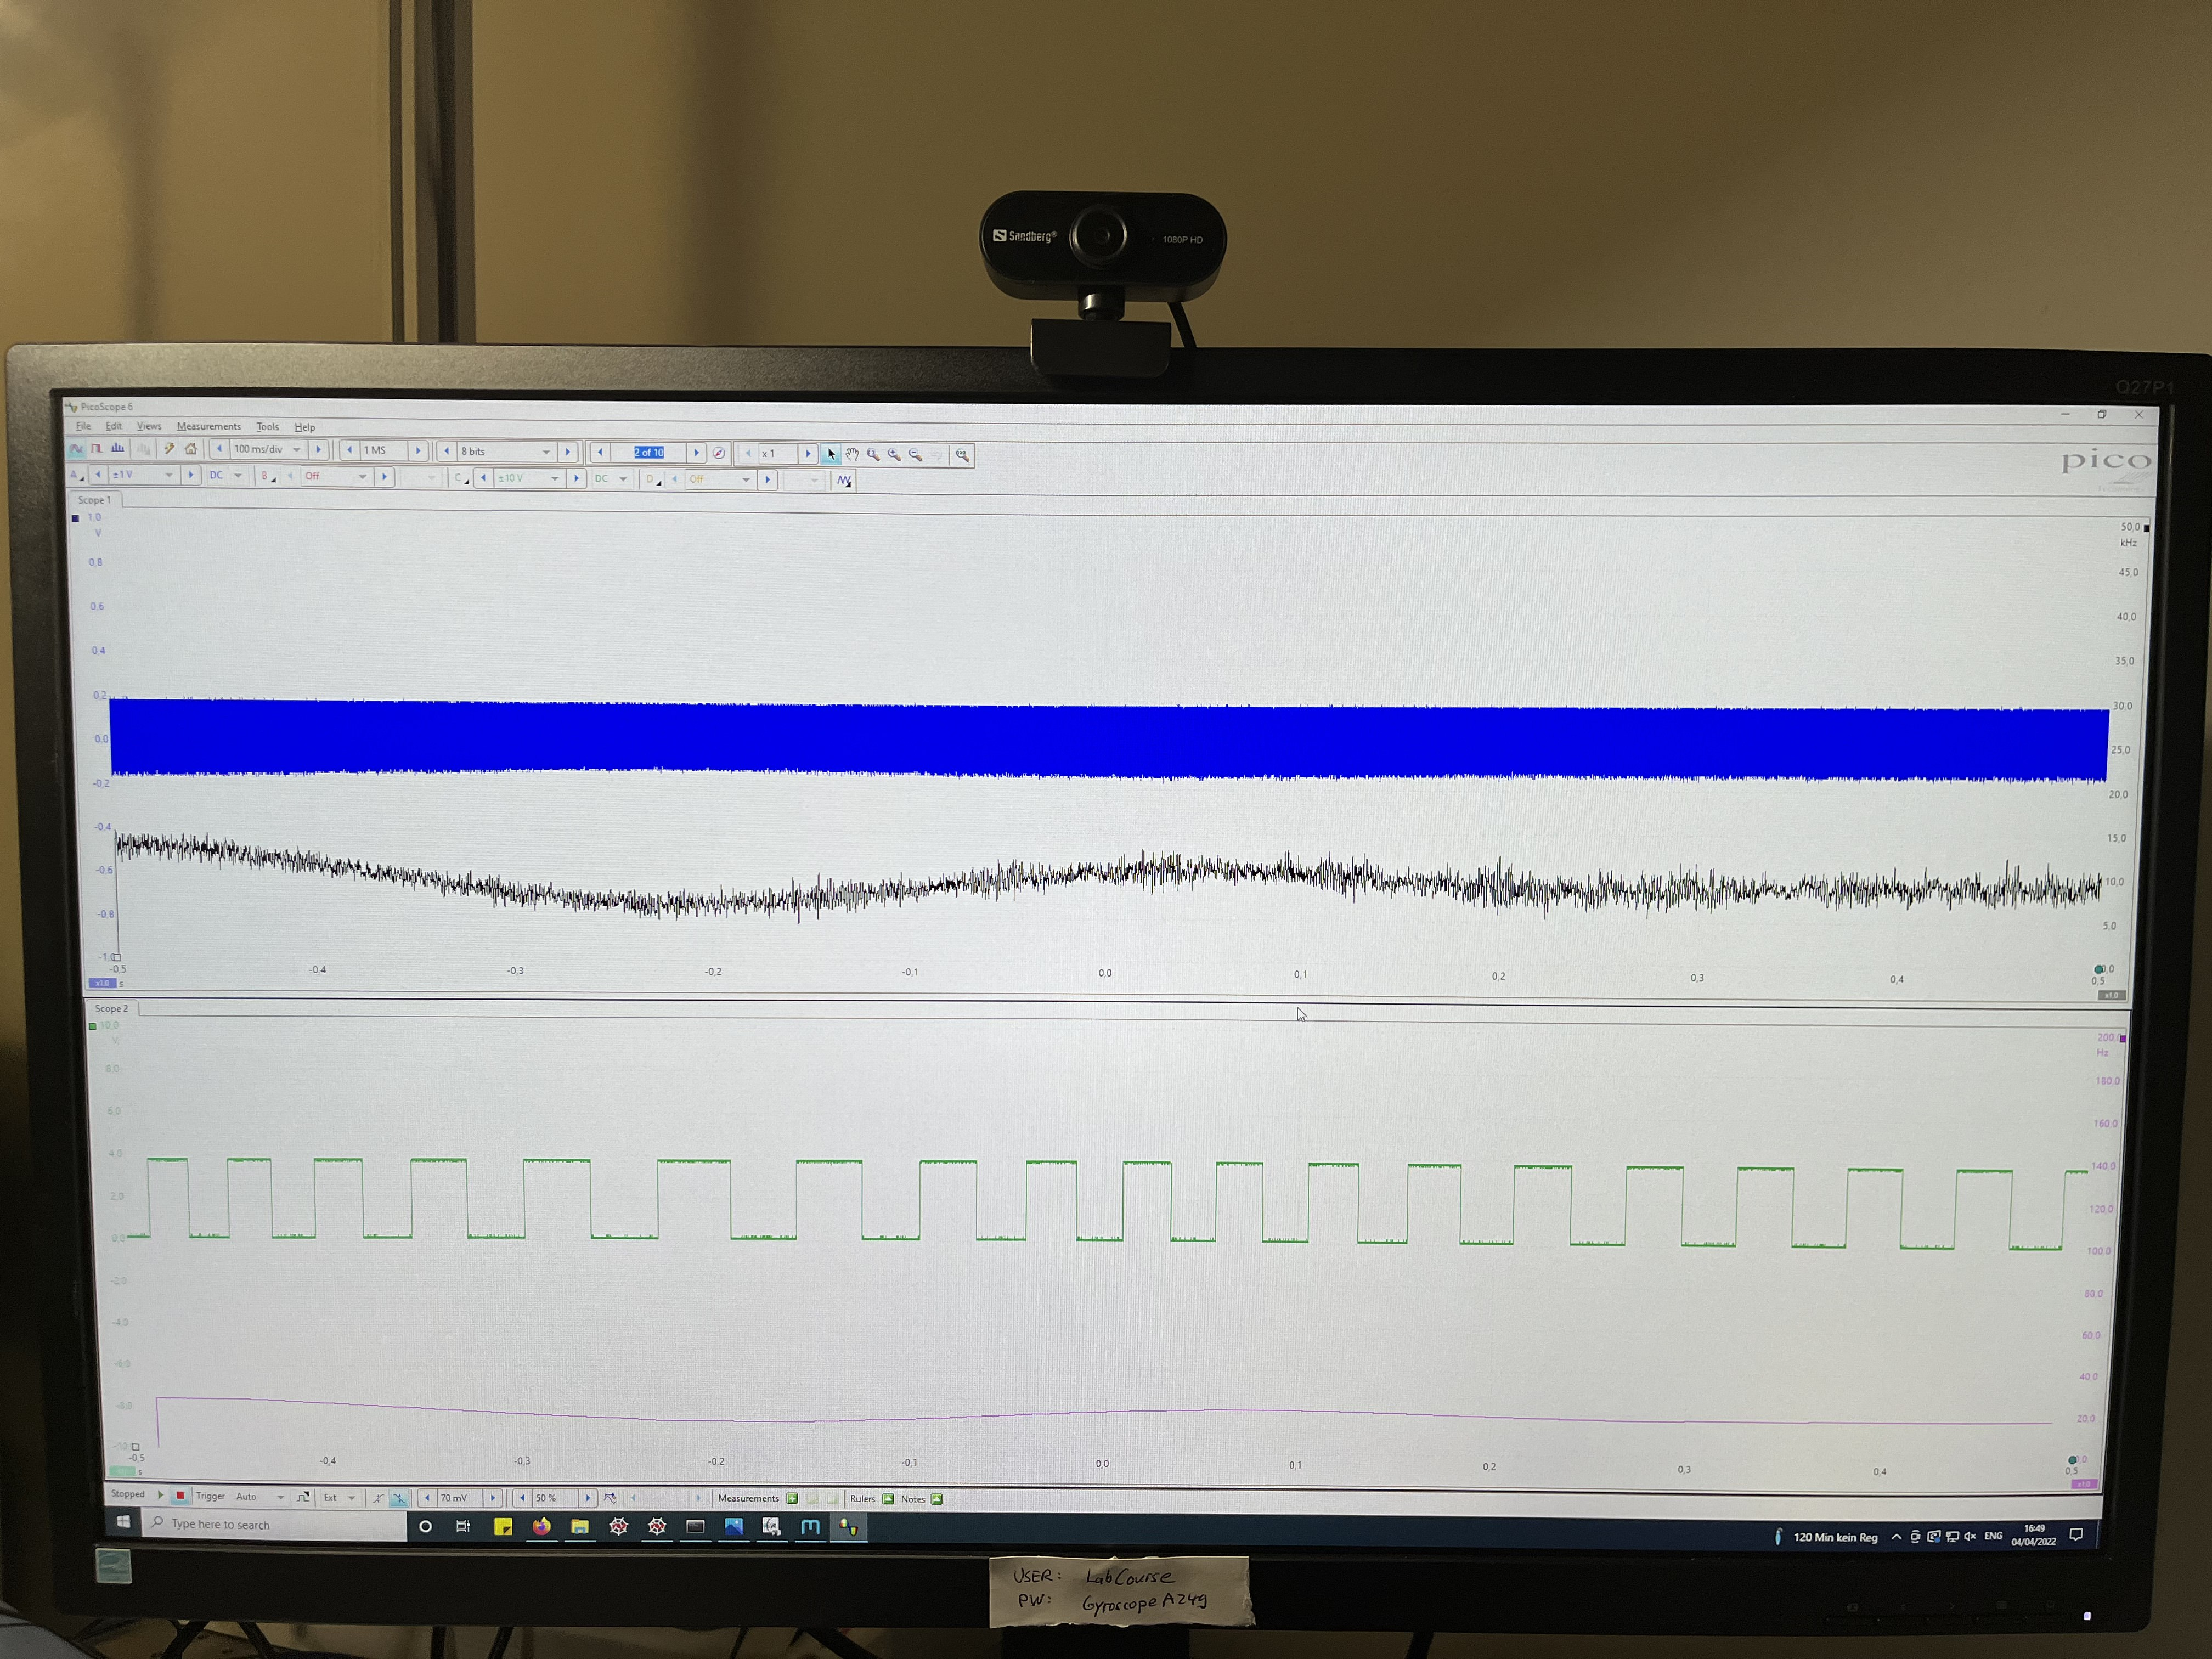
\includegraphics[width=0.8\columnwidth]{software_picture.jpg}
% 	\caption{An example output from the AOM software used to monitor the beat frequency.}
% 	\label{fig:exp_setup_software}
% \end{figure*}

To rotate the table, we used a rotary encoder that sends a voltage signal that controls the rotation rate of the table. The output 
was connected to the AOM software so that the rotation rate can be observed simultaneously with the observed beat frequency when 
measuring the Sagnac frequency and the Allan deviation. Fig. \ref{fig:exp_setup_gyroscope} shows the gyroscope used in this experiment.

\begin{figure*}[h!]
	\centering
	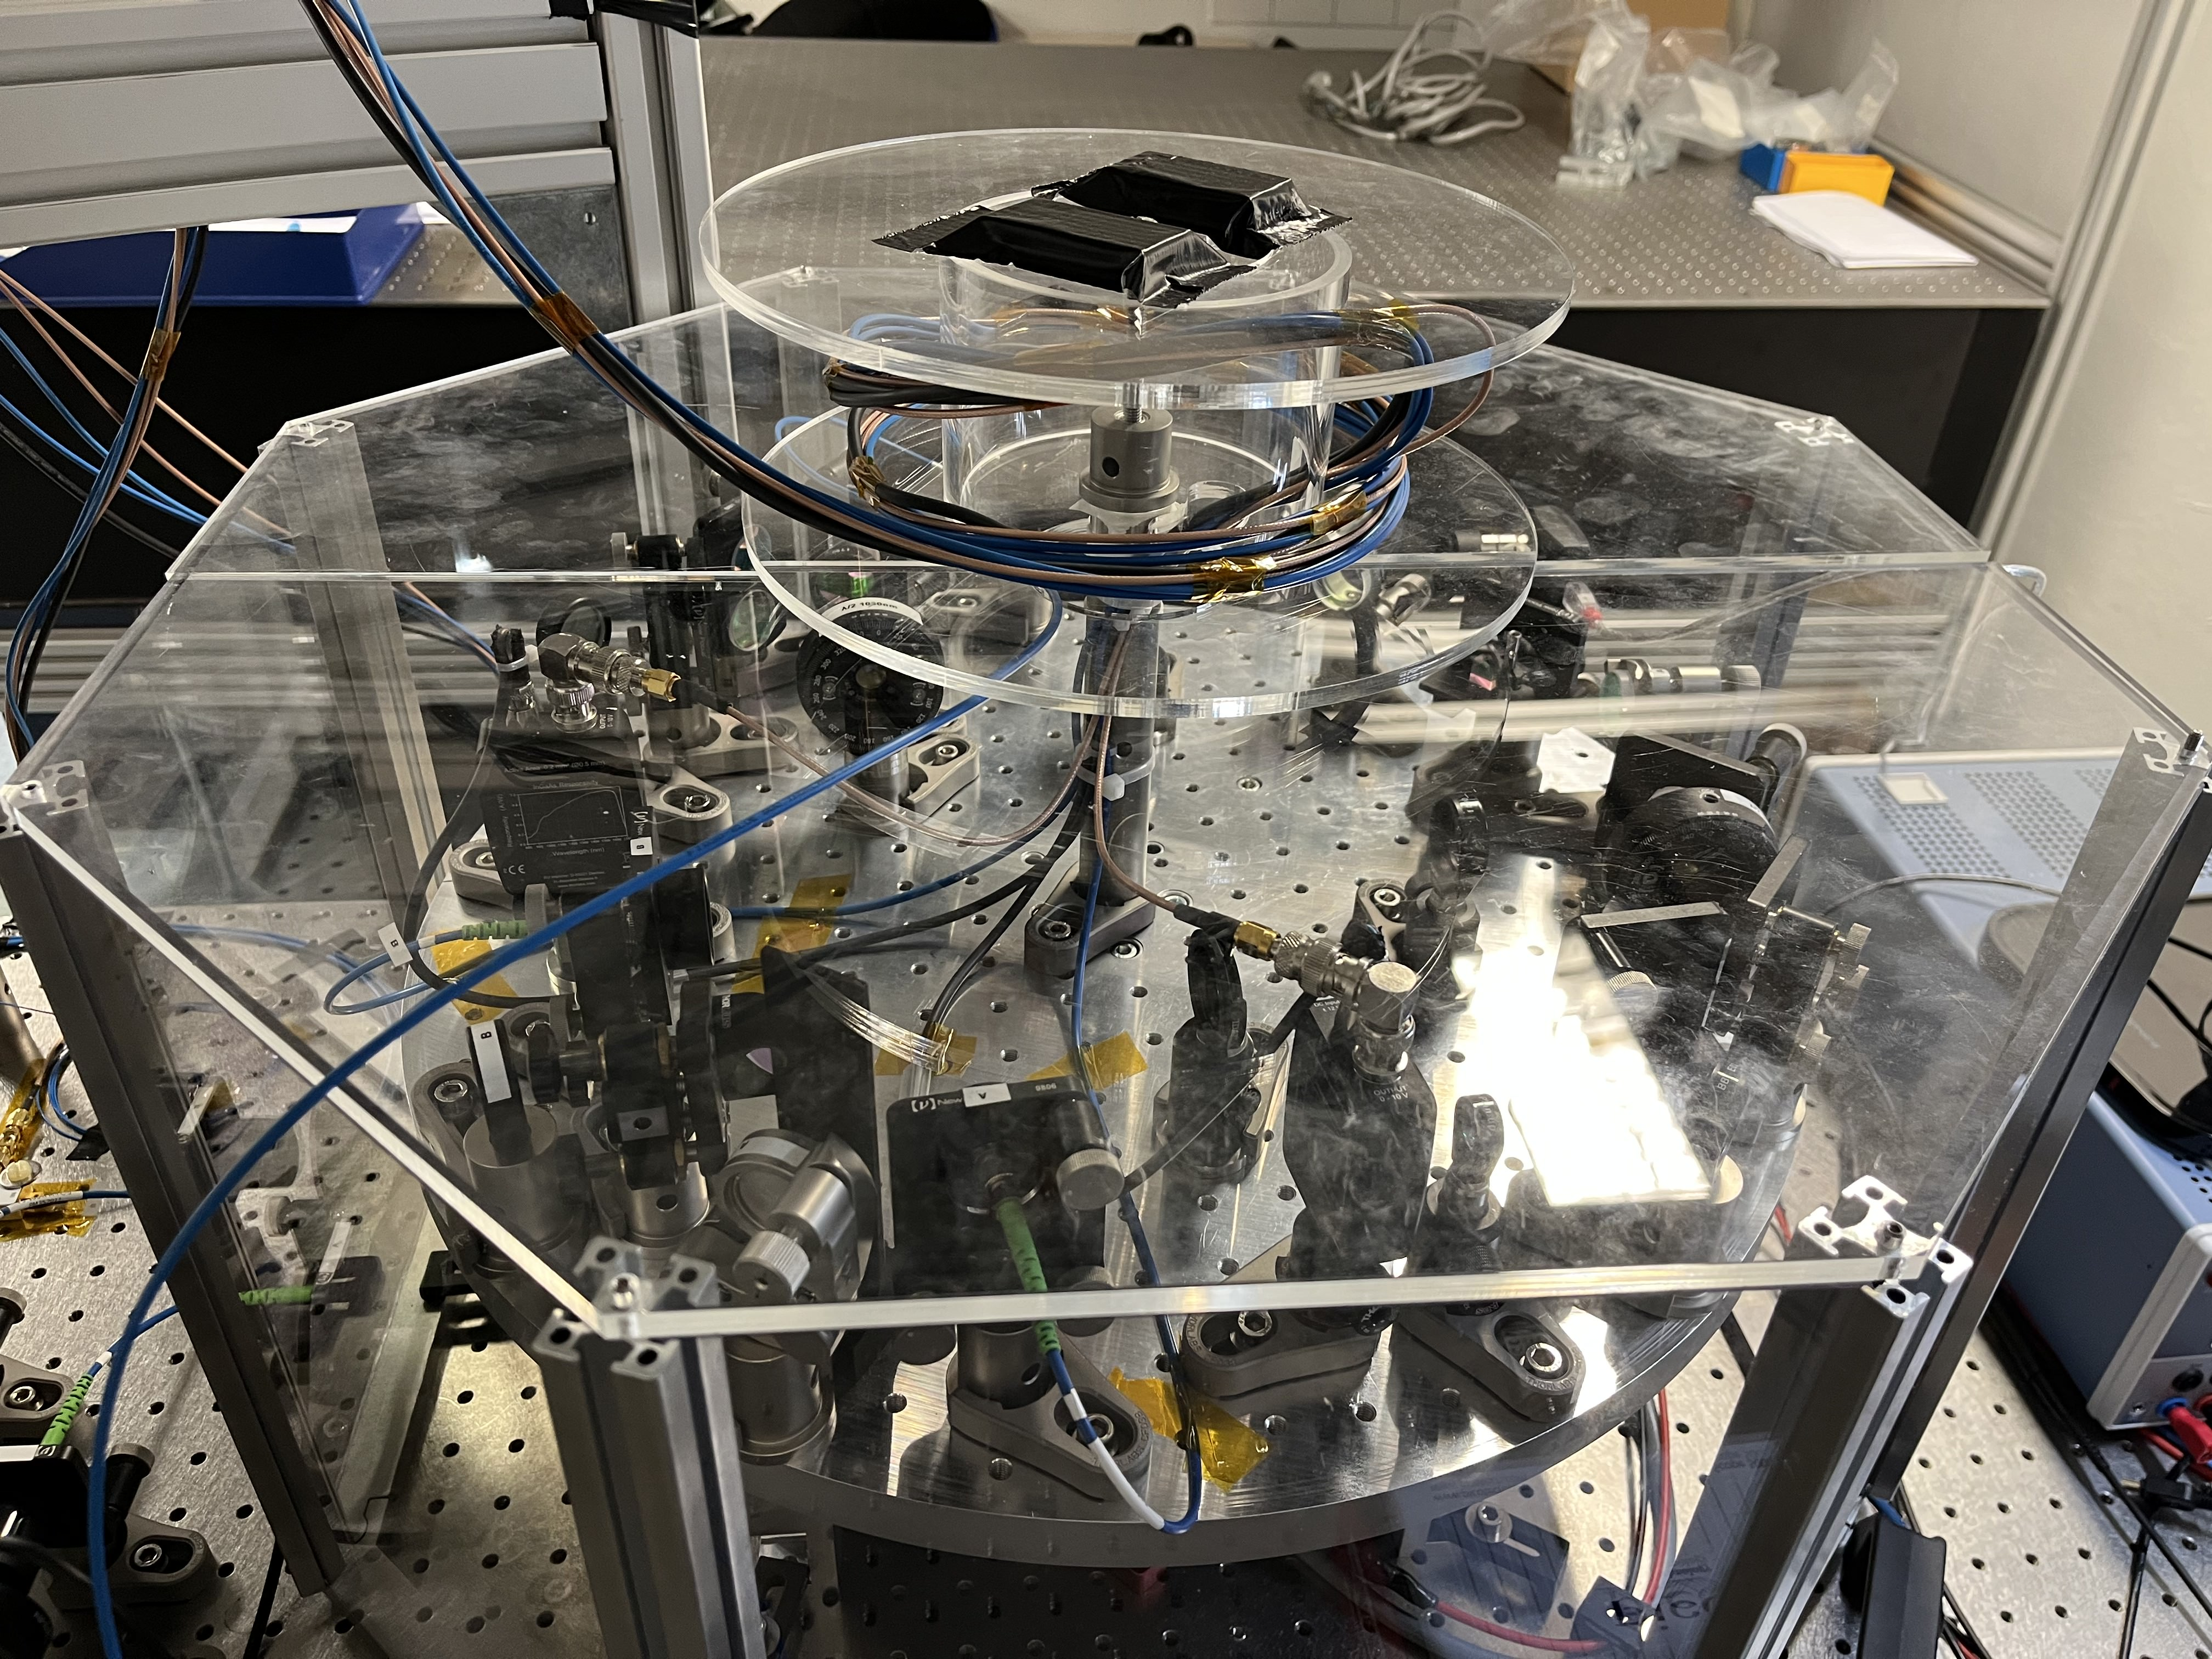
\includegraphics[width=0.6\columnwidth]{gyroscope_picture.jpg}
	\caption{The ring cavity laser gyroscope used in this experiment.}
	\label{fig:exp_setup_gyroscope}
\end{figure*}

\section{Procedure}

\subsection{Free Spectral Range}

We first measured both the signal of the laser input and after the laser
has passed through the ring cavity system. The window was adjusted until three resonance peaks and their corresponding sidebands
were observed. See Fig. \ref{fig:threeres_raw} the observed raw signal. 

\begin{figure*}[h!]
	\centering
	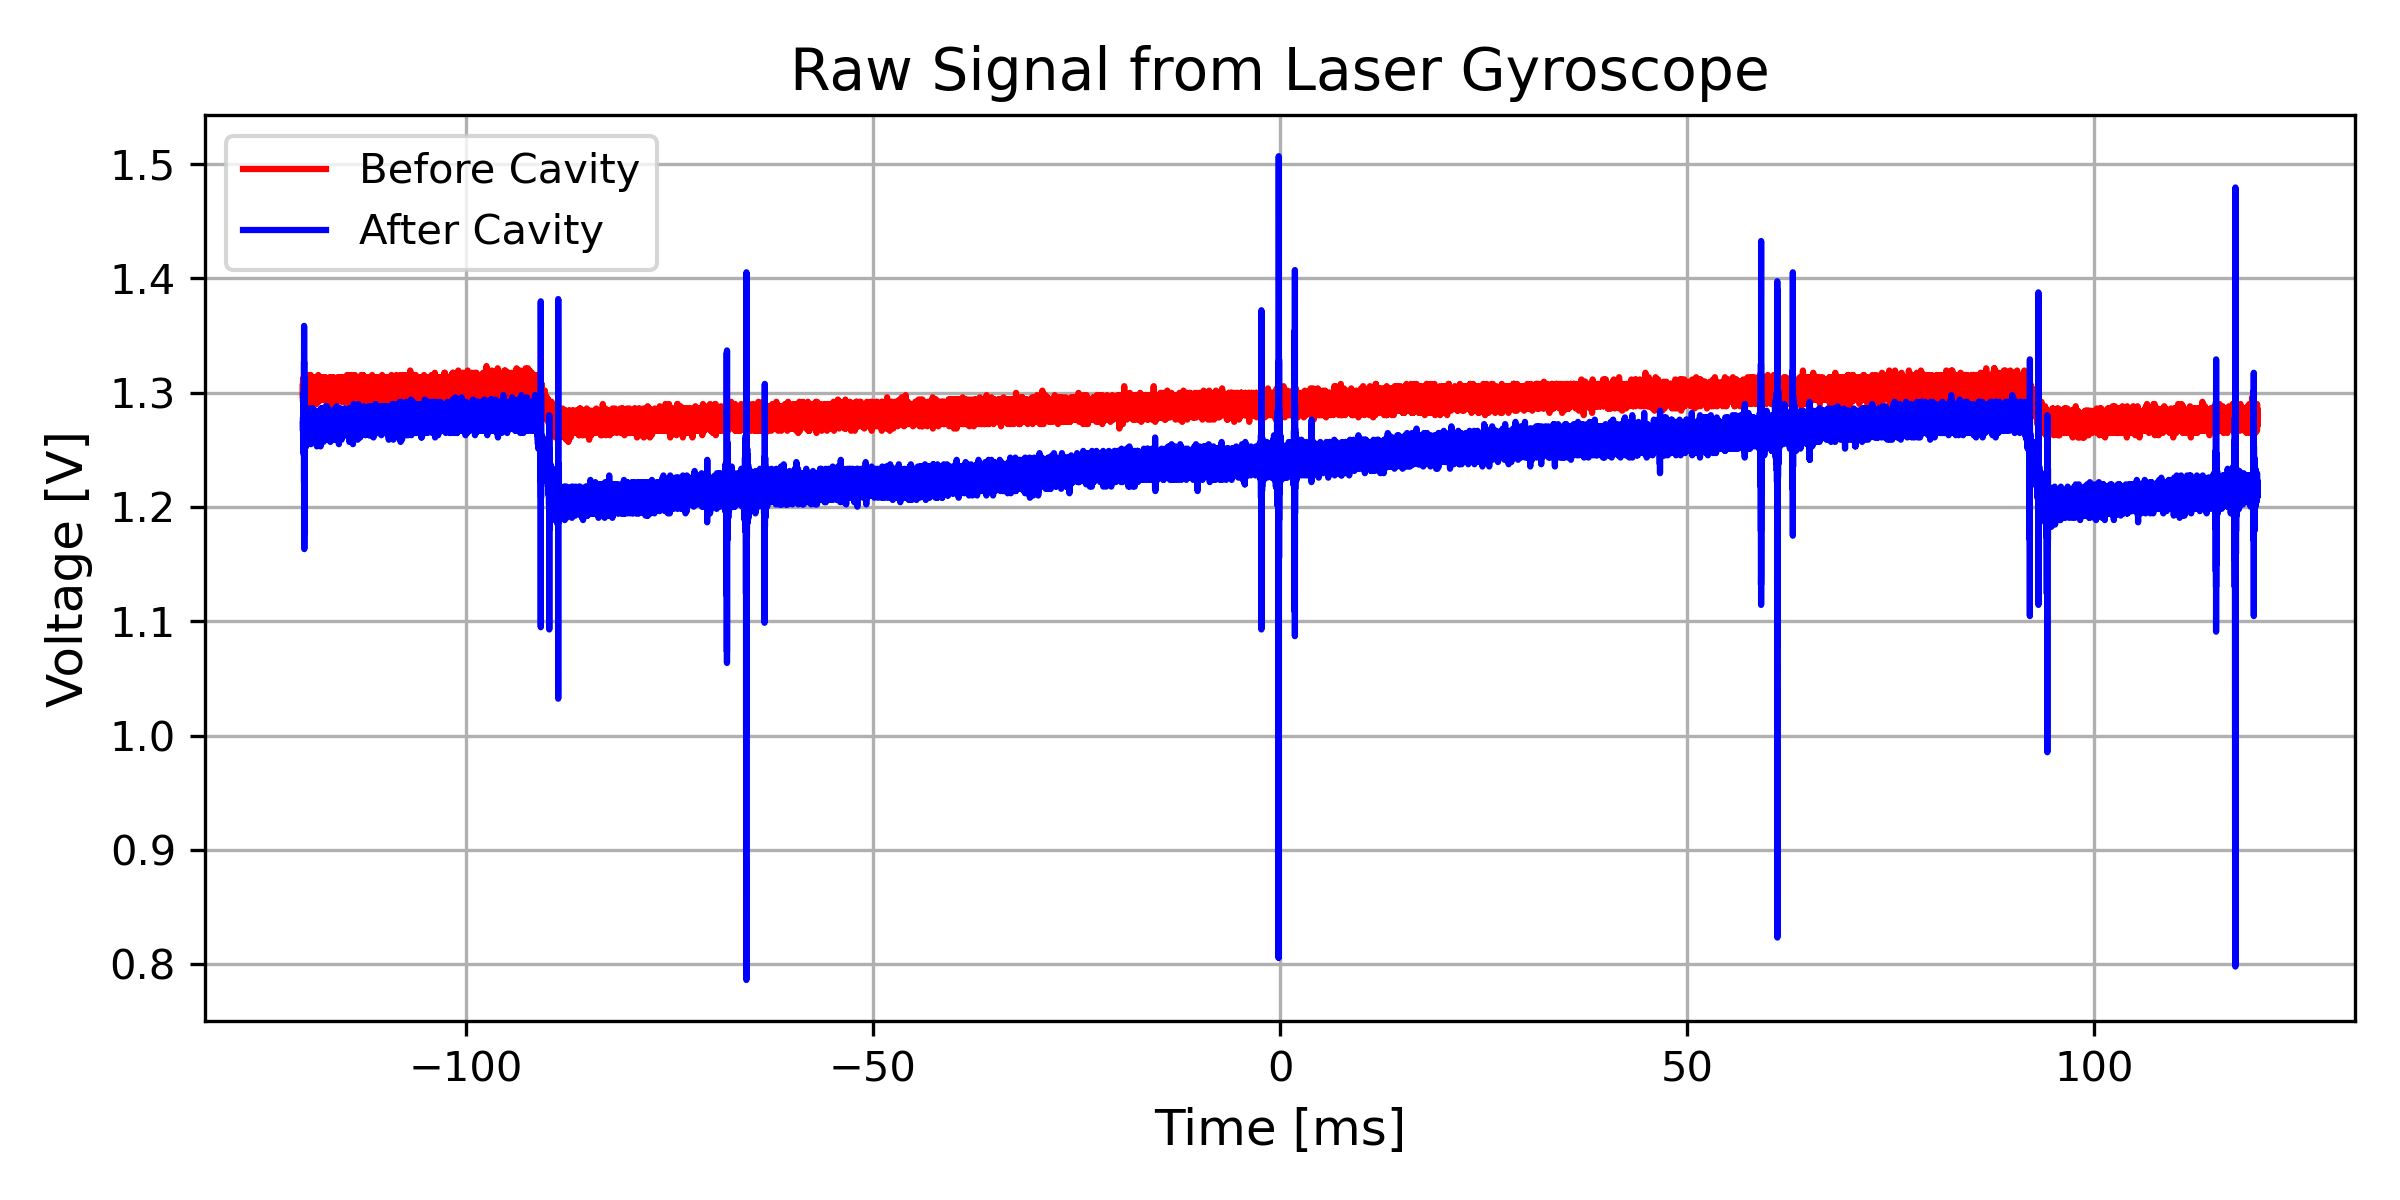
\includegraphics[width=0.8\columnwidth]{threeres_raw.png}
	\caption{Raw signal input from the laser before and after passing through the ring 
			cavity system.}
	\label{fig:threeres_raw}
\end{figure*}

As the raw data was provided in the time domain, we converted the time axis into a frequency axis.
In order to do so, we use the fact that the modulation frequency from the EOM was $\Omega = \SI{10}{\mega\hertz}$,
and we determined the width in time between the peaks and the sidebands to obtain a conversion time between 
the two axes. The error of the conversion time was obtained purely statistically by using the standard error of the mean. \par 

From this conversion time, we obtained the free spectral range as the peak-to-peak difference between
the resonance peaks.The error in the free spectral range was considered by observing the approximate 
full-width half-maximum of each peak. We then took the weighted average of the free spectral ranges to obtain an averaged
free spectral range. \par 

We then evaluated the cavity perimeter from Eq. \ref{eq:fsr} for each free spectral range that we have observed.
We compared our obtained results with the measured value of the cavity perimeter
 $P_{\text{meas}} = \SI{0.990\pm 0.005}{\meter}$ obtained from Ref. \cite{Groh2021}. 


\subsection{PDH Error Signal and PID Optimization} \label{sec:pdh_err_procedure}

To observe the error signal generated from PDH locking, we observed the combined signal generated from the fast and slow PID controller. 
Fig. \ref{fig:errsig_raw} shows the raw signal obtained from the PDH error. \par 

\begin{figure*}[h!]
	\centering
	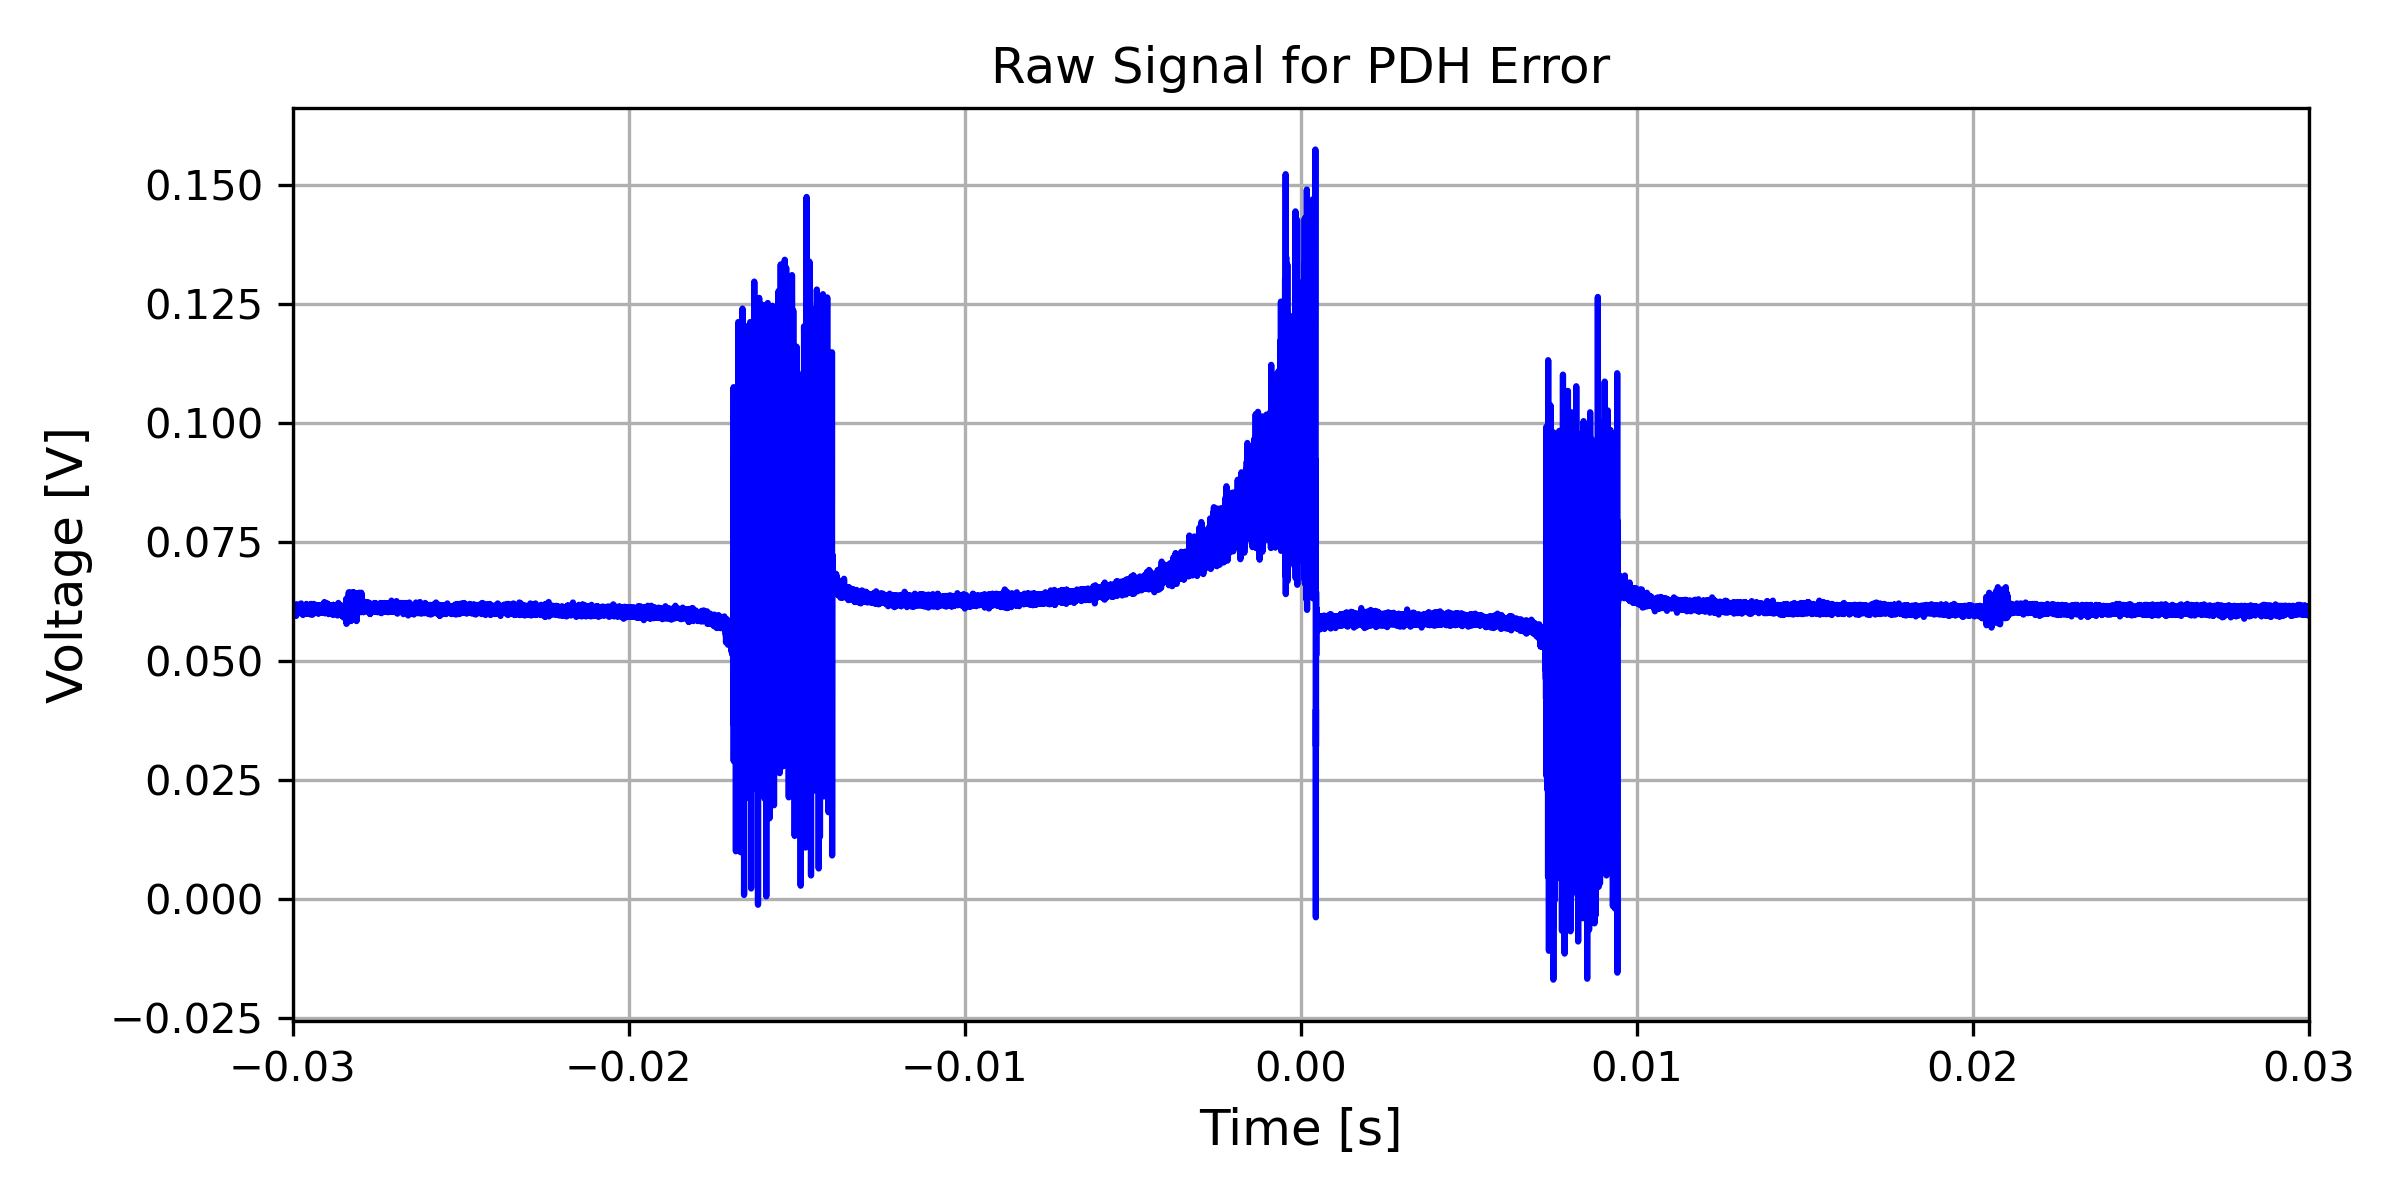
\includegraphics[width=0.8\columnwidth]{raw_err_sig.png}
	\caption{Raw Signal from PDH locking using the fast and slow PID controller.}
	\label{fig:errsig_raw}
\end{figure*}

The corresponding data was then used to determine the linear fit of the error signal where the zero crossing and 
linear slope is present (i.e. near the middle of the observed error signal). 
This was performed by first filtering the data using \texttt{scipy.signal.sosfilt}, then using a least-squares fit with 
\texttt{numpy.polyfit}.Fig. \ref{fig:pdh_err_filt} shows the filtered data from the error signal generated by PDH locking. We observe that the shape of the signal closely
resembles that of Fig. \ref{fig:error-signal} as desired. 

 \begin{figure*}[h!]
	\centering
	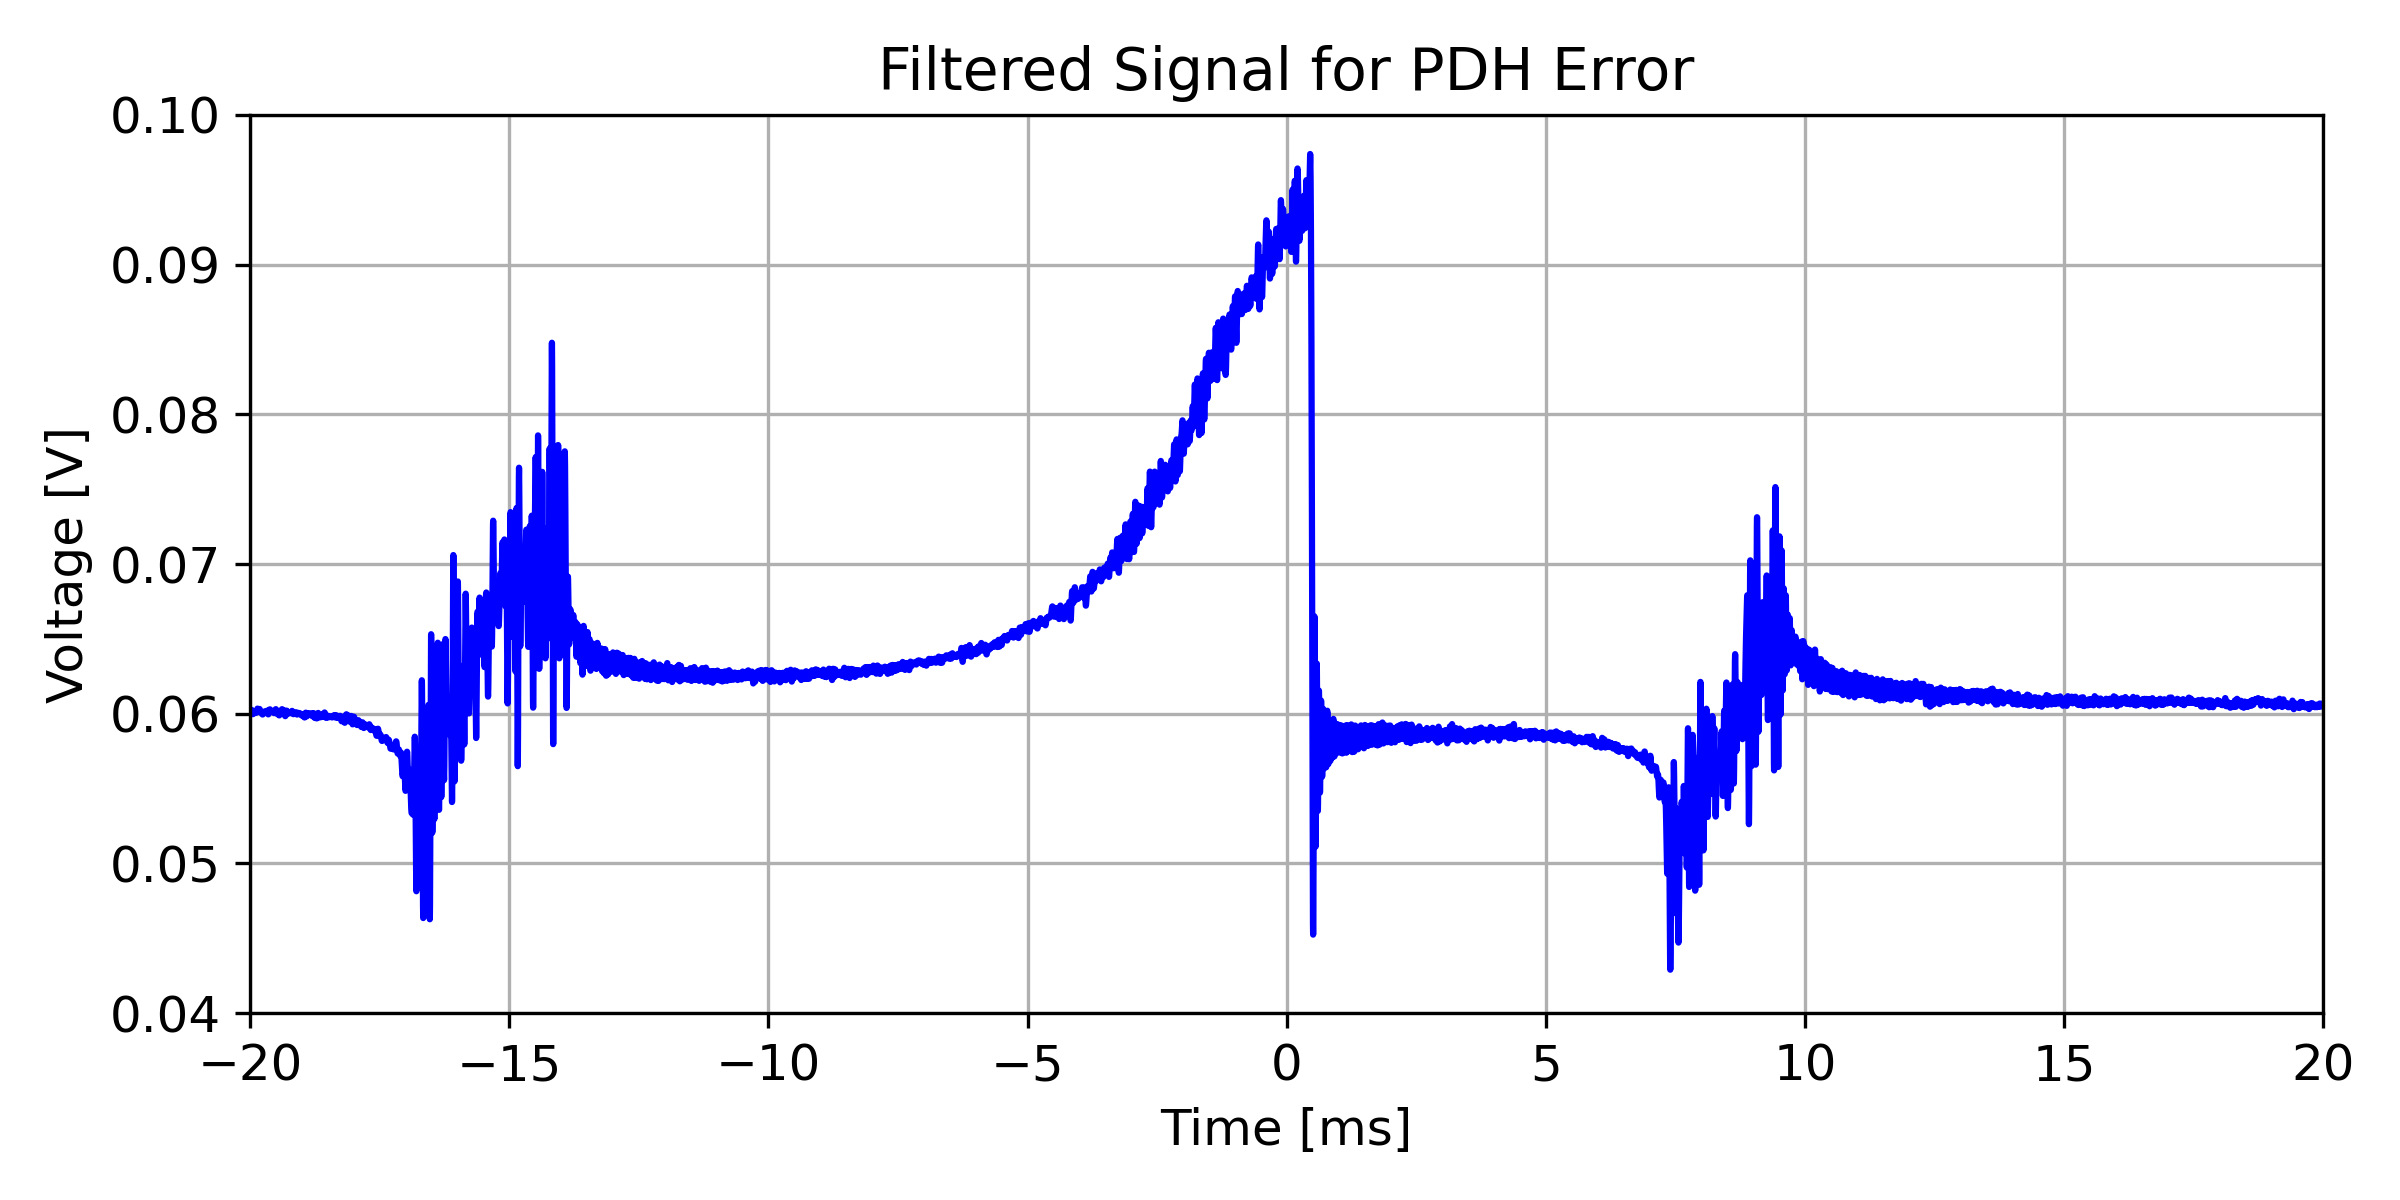
\includegraphics[width=0.8\columnwidth]{pdh_err_filt.png}
	\caption{Filtered signal from PDH locking. The behavior of the signal closely resembles that of the signal 
	shown in Fig. \ref{fig:error-signal}. }
	\label{fig:pdh_err_filt}
\end{figure*}


The error signal was then used to determine the optimal PID parameters that yield the most stable and large signal. In order to 
do this, the following parameters were modified: SLOW INT, FAST INT, DIFF GAIN, FAST DIFF / FILTER, SLOW GAIN, FAST GAIN, GAIN LIMIT, and OFFSET. The major parameters that influenced the signal were the SLOW INT, SLOW GAIN, FAST DIFF / FILTER and FAST GAIN. Modifying the SLOW INT and FAST DIFF caused the laser to be out of lock, whereas FAST GAIN decreased the noise observed in the signal. As we decreased the SLOW GAIN, we observed that the laser became more out of lock, allowing for the control of the laser locking. The OFFSET parameter adjusted the offset between the two signals. Table \ref{tab:pid_params} 
shows the optimal PID parameters used in the subsequent measurements which were both stable and yielded a strong signal strength. \par 

\begin{table}[h!]
	\centering
	\begin{tabular}{|c|c|}
		\hline 
		PID Parameter & Value \\ \hline
		SLOW INT & 25 \\ \hline
		FAST INT & 20K \\ \hline
		FAST DIFF / FILTER & 10M \\ \hline
		FAST GAIN & $\SI{6}{\decibel}$ \\ \hline
		GAIN LIMIT & 30 \\ \hline
	\end{tabular}
	\caption{The optimal PID parameters used for this experiment. The SLOW GAIN and FAST GAIN parameter values are not noted
	as specific values are not marked on the Moglabs PID controller.}
	\label{tab:pid_params}
\end{table}

When performing laser locking, we further needed to consider the systematics due to the environment. 
Any small disturbance such as clapping, tapping the desk, moving the cables or even walking influenced the 
degree of locking for the laser. Other factors such as the temperature fluctuations in the room may have caused the 
laser to be out of lock as well. In order to verify that we were obtained the correct resonant mode when optimizing 
the PID parameters (i.e. the TEM$_{\mathrm{010}}$ mode), we used a camera located on the rotation table. An image of the 
resulting mode obtained when locking can be seen in Fig. \ref{fig:tem00-lock}. \par 


\begin{figure}[htpb]
    \centering
    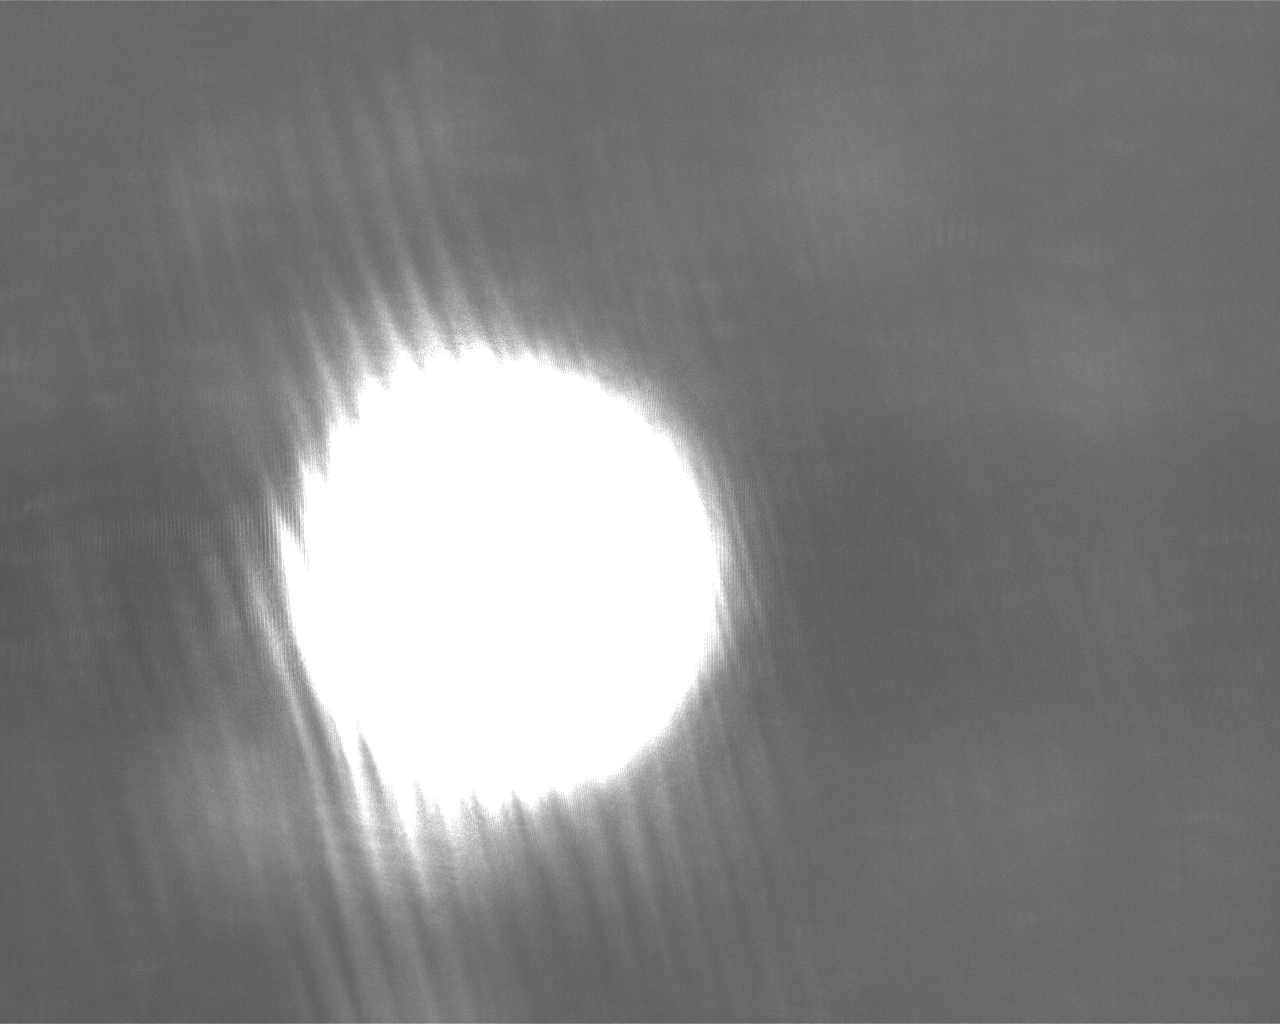
\includegraphics[width=0.6\columnwidth]{tem00_lock}
    \caption{The Fundamental $\mathrm{TEM}_{0, 0}$ Gaussian mode.}
    \label{fig:tem00-lock}
\end{figure}	

\subsection{Cavity Ring-Down}

\begin{figure}[htpb]
    \centering
    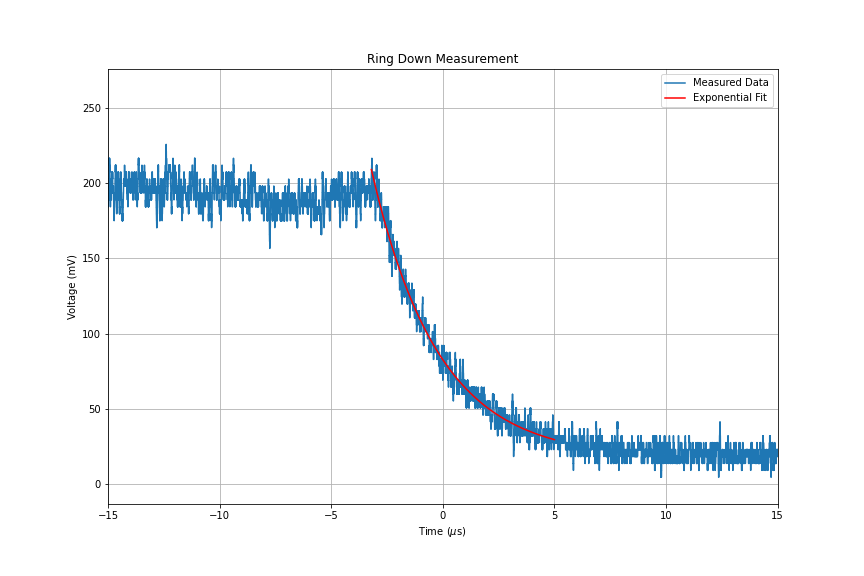
\includegraphics[width=0.7\textwidth]{ring-down}
    \caption{Exponential decay of power in the cavity after swithcing it off.}
    \label{fig:ring-down}
\end{figure}

As discussed in the \ref{sec:ring-down}, here we measure the exponential decay of power within the cavity after the ``switch" is turned off. After setting the photodiode channel to the appropriate height, trigger mode was set to single. The laser beam is then switched off using the front panel control of the AOM driver. We notice an exponential decay, as seen in Fig. \ref{fig:ring-down}. Several measurements were taken out which twelve were analyzed. Rest of the figures can be found in the Appendix \ref{chap:appendix}. The data was ananlysed in \texttt{Python} and curve fitting was done using the following function

\begin{equation}
		f(t) = a \exp\left(-\frac{t}{t_{dec}}\right) + c,
\end{equation}
where $a$ is the amplitude, $t_{dec}$ is the decay constant and $c$ is a constant. The fitting was done using the function \texttt{scipy.optimize.curve-fit}. This function also gives us the error associated with the fit. Using the fit parameters, the decay constant can be computed using the Eqn. \ref{eqn:ring-down}. Using the value of decay constant, reflectivity was computed using the Eqn. \ref{eqn:reflec} and finesse of the cavity was computed using Eqn. \ref{eqn:finesse}. The weighted mean and error was calculated for the twelve different measurements. Error propagation was used in order to calculate the error associated with these quantities.


% \subsubsection{Locking}

% % need to have this figure here

% % \begin{figure}[htpb]
% %     \centering
% %     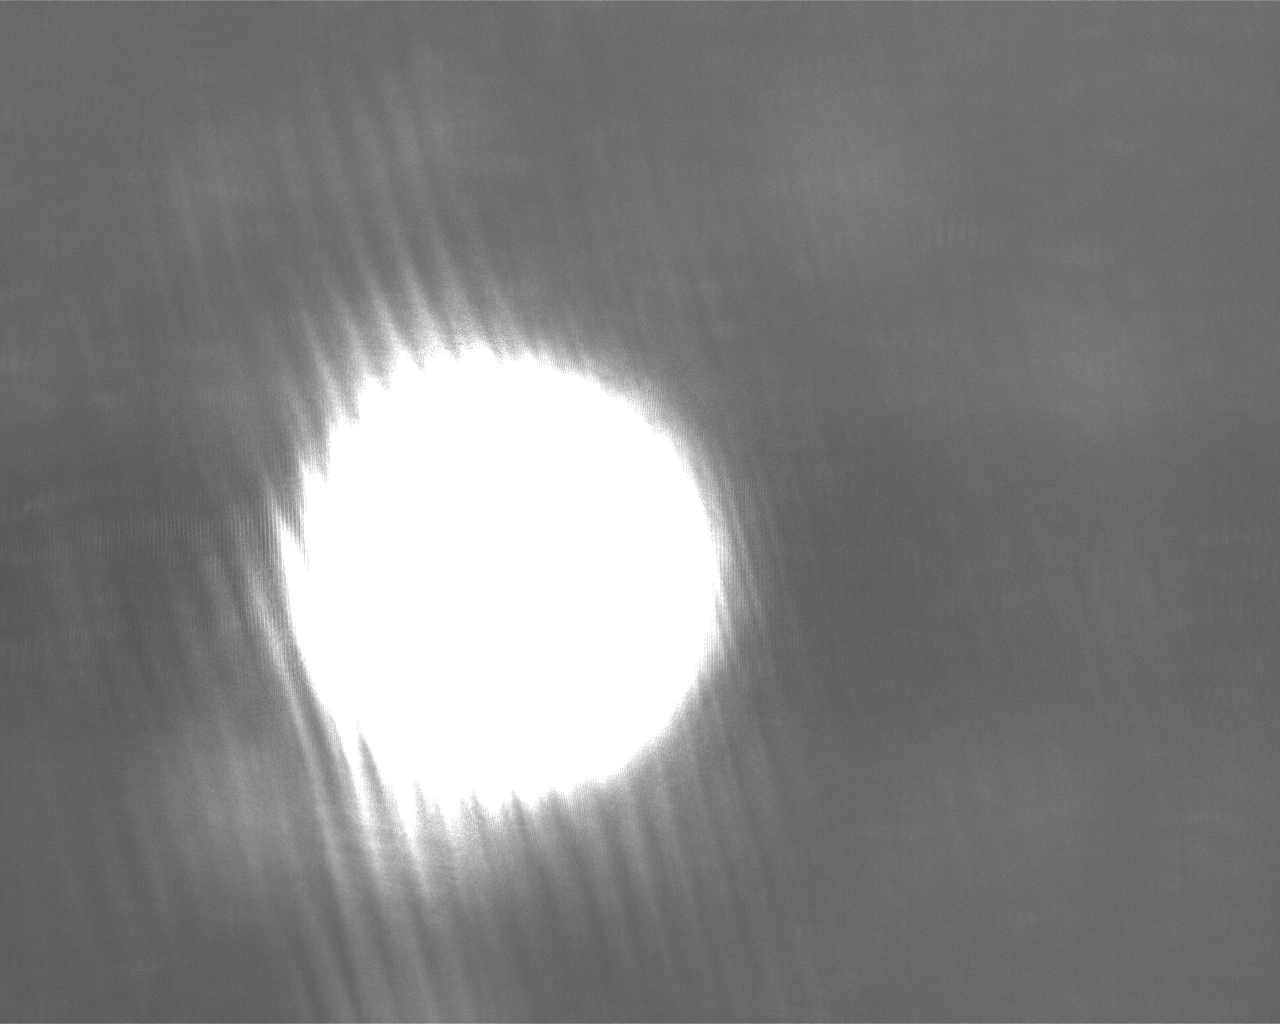
\includegraphics[width=0.6\textwidth]{tem00_lock}
% %     \caption{The Fundamental $\mathrm{TEM}_{0, 0}$ Gaussian mode.}
% %     \label{fig:tem00-lock}
% % \end{figure}	

\subsection{Scale Factor} \label{sec:scale_fact}
The gyroscope table was set into rotation, all the while making sure that the cavity was still locked. The oscilloscope channel was used to read the frequency. In order to get the frequency in Hz, the encoder rate of 10,000 needs to be taken into account. Since one complete rotation corresponds to 10,000 counts, the recorded values need to be divided by 10,000. Since this is the angular frequency of the table, in order to get the rotation rate in $\si{\hertz}$, the final fit value is divided by a factor of $2 \pi$ in order to get the correct dimensions. 

The beat signal was recorded from another channel and evaluated for five different voltages, which correspond to five different rotation rates. Higher rotation rates lead to highly unstable cavity, with stability of the lock not lasting more than 2-3s. Hence, lower rotation rates were preferred for a much more reliable data. Nevertheless, even at low rotation rates, the cavity falls out of lock and we had to re-lock it and continue taking readings. Another interesting thing to note is that this lock could be broken with slight disturbances like banging the table or moving the chair. 

As an example, the unfiltered data for beat frequency at 1.5V is shown in Fig. \ref{fig:unfiltered-Sagnac}. In order to extract usable data from this, first loose upper and lower bounds were set to make sure that unreasonably high and low values do not contribute. From \texttt{scipy.signal}, the package \texttt{savgol-filter} was used to filter the data. The filtered data is shown in Fig. \ref{fig:filtered-Sagnac}. 

% \begin{figure}
% 	\centering
% 	\begin{subfigure}[!h]{0.5\textwidth}
% 		\centering
% 		\includegraphics[width=0.8\linewidth]{unfiltered_Sagnac_15}
% 		\caption{Unfiltered data of Sagnac beat frequency with 1.5V applied to the rotation table.}
% 		\label{fig:unfiltered-Sagnac}
% 	\end{subfigure}
% 	\begin{subfigure}[!h]{0.5\textwidth}
% 			\centering
% 			\includegraphics[width=0.8\linewidth]{filtered_Sagnac_15}
% 			\caption{Filtered data of Sagnac beat frequency with 1.5V applied to the rotation table.}
% 			\label{fig:filtered-Sagnac}
% 	\end{subfigure}
% 	\caption{Unfiltered and filtered data for 1.5V.}
% \end{figure}

\begin{figure*}[h!]
	\centering
	\subfloat[Unfiltered data of Sagnac beat frequency with 1.5V applied to the rotation table. \label{fig:unfiltered-Sagnac}]{{\includegraphics[width=0.8\columnwidth]{unfiltered_Sagnac_15}}}
	\quad
	\centering
	\subfloat[Filtered data of Sagnac beat frequency with 1.5V applied to the rotation table. \label{fig:filtered-Sagnac}]{{\includegraphics[width=0.8\columnwidth]{filtered_Sagnac_15}}}
	\caption{Unfiltered and filtered data for 1.5V.}
	%\label{fig:}
\end{figure*}

Similarly, in order to get the rate of rotation of the table, the data was first filtered. As an example for this, we look at the data corresponding to 2V. This can be seen in Fig. \ref{fig:filter-freq}. 

\begin{figure*}[h!]
	\centering
	\subfloat[Unfiltered data of rate of rotation of table  with 2V. \label{fig:unfiltered-Sagnac}]{{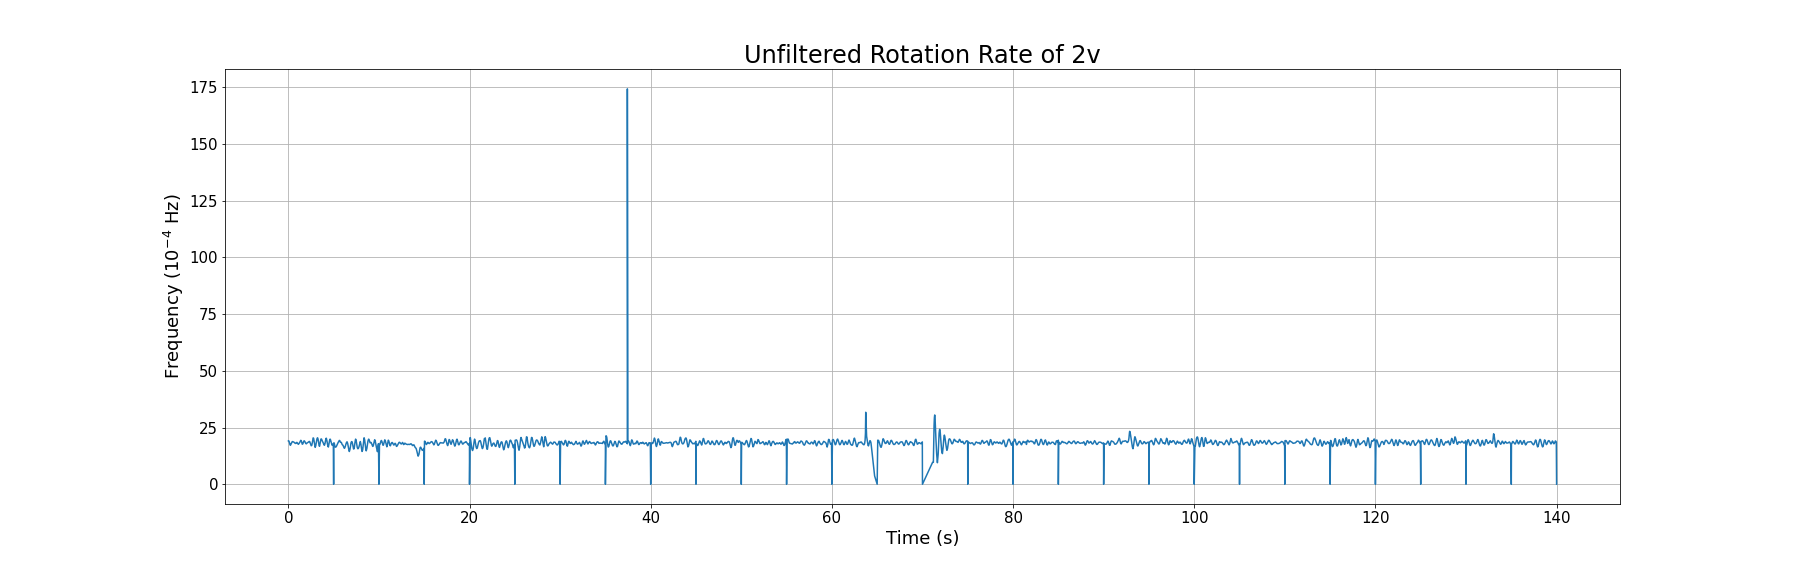
\includegraphics[width=0.8\columnwidth]{unfiltered_freq_2}}}
	\quad
	\centering
	\subfloat[Filtered data of rate of rotation of table  with 2V. \label{fig:filtered-Sagnac}]{{\includegraphics[width=0.8\columnwidth]{filtered_freq_2}}}
	\caption{Unfiltered and filtered data for 2V.}
	\label{fig:filter-freq}
\end{figure*}

% \begin{figure}
% 		\centering
% 		\begin{subfigure}[!h]{0.5\textwidth}
% 				\centering
% 				\includegraphics[width=0.8\linewidth]{unfiltered_freq_2}
% 				\caption{Unfiltered data of rate of rotation of table  with 2V.}
% 		\end{subfigure}
% 		\begin{subfigure}[!h]{0.5\textwidth}
% 				\centering
% 				\includegraphics[width=0.8\linewidth]{filtered_freq_2}
% 				\caption{Filtered data of rate of rotation of table  with 2V.}
% 		\end{subfigure}
% 		\caption{Unfiltered and filtered data for 2V.}
% 		\label{fig:filter-freq}
% \end{figure}

In order to extract the Sagnac frequency and the rate of rotation, the average of the filtered data was taken. Averages were calculated for six different rotation rates. These were then plotted against each other and a fit was made using the package \texttt{np.polyfit}. A standard systematic error of $\pm 2500 \text{Hz}$ was taken in order to account for the noise and fluctuations. Statistical error was computed using assuming a gaussian distribution and error propagation was done. 


\subsection{Allan Deviation}

Finally, we measured the Allan deviation of the laser gyroscope. We performed the same procedure as with the scale factor measurement. 
Using the same PID parameters as before, we set the rotation frequency to rotate with $\SI{0.75}{\volt}$, so that the laser will 
remain locked as long as possible. The gyroscope was rotated until the cable connecting the gyroscope did not extend or contract
any further, then the same analysis was performed in the opposite rotation direction. The measurement was taken continuously for 
approximately 1.5 hours. The unprocessed time series for the frequency measurement can be seen in Fig. \ref{fig:allan_ts_raw}. \par 


\begin{figure*}[h!]
	\centering
	\includegraphics[width=0.8\columnwidth]{allan_ts_raw.png}
	\caption{Unprocessed time series obtained from Allan deviation measurements. We observe large
			spikes at numerous locations as well as regions with zero frequency.}
	\label{fig:allan_ts_raw}
\end{figure*}

From the raw data, we first removed any measurements that were taken while the laser was unlocked and when the 
rotation of the table was switched. We then apply filtering towards our data using \texttt{scipy.signal.sosfilt} to remove
fluctuations of the signal. Fig. \ref{fig:allan_ts_filt} shows the measured data after filtering. We observe that the signal of 
the Sagnac frequency differs in the region $t \in [1800, 3800]$ as compared to the other regions, yielding an average frequency
of $\sim \SI{2000}{\hertz}$ larger than the others. This is due to the fact that we have rotated the table counter-clockwise
for that duration. The rotation rate of the table, however, was kept the same, and as such this has no impact in the 
calculation of the Allan deviation. \par 

\begin{figure*}[h!]
	\centering
	\includegraphics[width=0.8\columnwidth]{allan_ts_filt.png}
	\caption{Time series of Allan deviation measurement after filtering and removing unwanted data measurements.}
	\label{fig:allan_ts_filt}
\end{figure*}

We then performed the same procedure as with the Pre-lab tasks in Sec. \ref{sec:prelab_allan_dev} to determine the Allan deviation, namely to first determine the frequency spectrum of the signal using \texttt{scipy.fft} before passing through the frequency data into \texttt{allantools.oadev}
to obtain the Allan deviation for each integration time $\tau$. We also determined the shot-noise limited time $\tau$ by observing the time duration in which the instability of the 
measurement starts. For the rotation frequency of the table, we followed the same procedure from Sec. \ref{sec:scale_fact}. \par 

% $\Omega = \SI{5.95\pm 0.75}{\hertz}$


\chapter{Results and Discussion}

\section{Free Spectral Range} \label{sec:fsr}

Table \ref{tab:mod_times} shows the corresponding conversion time obtained from each sideband using the modulation frequency of $\SI{10}{\mega\hertz}$.
The mean conversion time that we obtained was $\SI{2.104 \pm 0.066}{\milli\second}$ which is the conversion time
that we used to determine the free spectral range. Fig. \ref{fig:res_peaks} shows the corresponding resonant peaks in both the time and frequency axis. \par


\begin{table}[h!]
	\centering
	\begin{tabular}{|c|c|}
		\hline 
		Sideband & Conversion time [ms] \\ \hline
		1 & 2.385 \\ \hline
		2 & 2.226 \\ \hline
		3 & 2.110 \\ \hline
		4 & 2.003 \\ \hline
		5 & 1.998 \\ \hline
		6 & 1.900 \\ \hline
		\textbf{Mean} & \textbf{$2.104 \pm 0.066$} \\ \hline
	\end{tabular}
	\caption{The conversion time determined from each sideband with the three resonant peaks obtained from Fig. \ref{fig:threeres_raw}.
	\hl{Fix table width}}
	\label{tab:mod_times}
\end{table}


\begin{figure*}[h!]
	\centering
	\subfloat[]{{\includegraphics[width=0.45\columnwidth]{res_peaks_time.png}}}
	\quad
	\centering
	\subfloat[]{{\includegraphics[width=0.45\columnwidth]{res_peaks_freq.png}}}
	\caption{The observed resonant peaks from the ring cavity in the laser gyroscope. (a) and (b) show the 
	same plot in the time and frequency domain respectively.}
	\label{fig:res_peaks}
\end{figure*}

From the obtained conversion time, we obtained two values of the free spectral range from the peak-to-peak difference
between each resonance peak. Correspondingly we also obtained two values for the cavity perimeter. Table \ref{tab:fsr_peri} shows the 
obtained free spectral range and cavity perimeter for each peak-to-peak difference as well as their weighted average.


\begin{table}[h!]
	\centering
	\begin{tabular}{|c|c|c|}
		\hline 
		Peak & $\delta\nu_{\mathrm{FSR}}$ [$\si{\mega\hertz}$] & Cavity Perimeter [$\si{\centi\meter}$]\\ \hline
		1-2 & $310.60 \pm 0.12$ & $96.587 \pm 0.039$ \\ \hline
		2-3 & $291.12 \pm 0.11$ & $103.050 \pm 0.040$ \\ \hline
		\textbf{Mean} & \textbf{$299.778 \pm 0.083$} & \textbf{$99.760 \pm 0.028$} \\ \hline
	\end{tabular}
	\caption{The free spectral range $\delta\nu_{\mathrm{FSR}}$ and the cavity perimeter $P$ obtained for each
			peak-to-peak. The weighted average is also shown. \hl{Fix table width}}
	\label{tab:fsr_peri}
\end{table}

When comparing the average cavity perimeter to the measured values given in Ref. \cite{Groh2021},
we observed that the experimental value were $1.52\sigma$ away. This indicates that the 
result we have obtained is in good, but not great agreement with the measured value. Such results may be caused by \par 

\section{PDH Error Signal}

Once applying the linear fit within the region of interest, we obtain 
the following parameters: $a = \SI{-1168 \pm 580}{\joule\per\second\squared}, \quad b = \SI{639.82 \pm 0.13}{\milli\joule\per\second}$
for a linear fit of $\epsilon_{\mathrm{fit}} = a t + b$. The filtered data within the region of interest
 with the linear fit is shown on Fig. \ref{fig:pdh_err_filt_fit}. As we can see, the slope is not truly vertical, indicating that there is some broadening of the 
 cavity linewidth, as $a \sim \sqrt{P_c P_s} \delta\nu_{\frac{1}{2}}$. 
 This is to be expected as thermal fluctuations as well as other disturbances can cause such broadening of the spectrum.  

 \begin{figure*}[h!]
	\centering
	\includegraphics[width=0.8\columnwidth]{pdh_err_filt_fit.png}
	\caption{The filtered signal from PDH locking in a zoomed-in region. The linear fit with associated fit parameters are 
	also shown.}
	\label{fig:pdh_err_filt_fit}
\end{figure*}

As we can observe from Fig. \ref{fig:pdh_err_filt}, the signal cannot truly exhibit the sharp peaks as observed in the 
Fig. \ref{fig:error-signal}. Such behavior is caused by the noise of the signal generated by the surrounding environment, as well as the
 oscillatory behavior of the signal, which causes the zero values to be oscillatory. Thus true peaks cannot be observed which 
 prevents us from applying a true linear fit to the data. \par 

\section{Cavity Ring-down}
The fit parameters and the errors associated with them are shown in Table \ref{tab:params}. The corresponding values of reflectivity and finesse is summarized in Table \ref{tab:ref-fin}. Lastly, the weighted mean and error were calculated and are shown in Table \ref{tab:mean-ref}. 

\begin{table}[!ht]
    \centering
    \begin{tabular}{|c|c|c|}
    \hline
        Amplitude & Decay constant ($\si{\micro\second}$) & Constant \\ \hline
        66.121 $\pm$ 0.200 & 3.049 $\pm$ 3.504 $\cross 10^{-6}$ & 17.995 $\pm$ 0.132 \\ \hline
        64.770 $\pm$ 0.152 & 2.911 $\pm$ 2.908 $\cross 10^{-6}$ & 20.862 $\pm$ 0.098 \\ \hline
        61.846 $\pm$ 0.144 & 2.978 $\pm$ 2.954 $\cross 10^{-6}$ & 18.201 $\pm$ 0.094 \\ \hline
        61.787 $\pm$ 0.124 & 2.915 $\pm$ 2.605 $\cross 10^{-6}$ & 18.501 $\pm$ 0.080 \\ \hline
        59.468 $\pm$ 0.136 & 3.098 $\pm$ 2.899 $\cross 10^{-6}$ & 18.823 $\pm$ 0.090 \\ \hline
        56.683 $\pm$ 0.129 & 2.887 $\pm$ 3.271 $\cross 10^{-6}$ & 19.797 $\pm$ 0.083 \\ \hline
        63.604 $\pm$ 0.156 & 3.031 $\pm$ 2.972 $\cross 10^{-6}$ & 16.951 $\pm$ 0.103 \\ \hline
        59.921 $\pm$ 0.167 & 2.899 $\pm$ 3.755 $\cross 10^{-6}$ & 19.726 $\pm$ 0.108 \\ \hline
        58.560 $\pm$ 0.140 & 2.959 $\pm$ 3.238 $\cross 10^{-6}$ & 19.142 $\pm$ 0.091 \\ \hline
        59.752 $\pm$ 0.142 & 2.839 $\pm$ 3.272 $\cross 10^{-6}$ & 20.856 $\pm$ 0.091 \\ \hline
        63.945 $\pm$ 0.160 & 3.008 $\pm$ 3.042 $\cross 10^{-6}$ & 17.469 $\pm$ 0.105 \\ \hline
        65.165 $\pm$ 0.132 & 2.970 $\pm$ 2.461 $\cross 10^{-6}$ & 17.501 $\pm$ 0.087 \\ \hline
    \end{tabular}
    \caption{Fit parameters.}
    \label{tab:params}
\end{table}

\begin{table}[!ht]
    \centering
    \begin{tabular}{|c|c|}
    \hline
        Reflectivity & Finesse \\ \hline
        0.999454 $\pm$ 1.516 $\cross 10^{-7}$ & 5757.144 $\pm$ 0.509 \\ \hline
        0.999428 $\pm$ 1.587 $\cross 10^{-7}$ & 5498.087 $\pm$ 0.486 \\ \hline
        0.999441 $\pm$ 1.552 $\cross 10^{-7}$ & 5623.439 $\pm$ 0.497 \\ \hline
        0.999429 $\pm$ 1.585 $\cross 10^{-7}$ & 5505.279 $\pm$ 0.487 \\ \hline
        0.999463 $\pm$ 1.491 $\cross 10^{-7}$ & 5850.284 $\pm$ 0.517 \\ \hline
        0.999423 $\pm$ 1.600 $\cross 10^{-7}$ & 5452.519 $\pm$ 0.482 \\ \hline
        0.999451 $\pm$ 1.524 $\cross 10^{-7}$ & 5723.937 $\pm$ 0.506 \\ \hline
        0.999426 $\pm$ 1.594 $\cross 10^{-7}$ & 5474.940 $\pm$ 0.484 \\ \hline
        0.999437 $\pm$ 1.562 $\cross 10^{-7}$ & 5587.268 $\pm$ 0.494 \\ \hline
        0.999414 $\pm$ 1.627 $\cross 10^{-7}$ & 5362.187 $\pm$ 0.474 \\ \hline
        0.999447 $\pm$ 1.536 $\cross 10^{-7}$ & 5680.210 $\pm$ 0.502 \\ \hline
        0.999440 $\pm$ 1.556 $\cross 10^{-7}$ & 5608.913 $\pm$ 0.496 \\ \hline
    \end{tabular}
    \caption{Reflectivity and Finesse of each measurement.}
    \label{tab:ref-fin}
\end{table}


\begin{table}[!ht]
    \centering
    \begin{tabular}{|c|c|}
    \hline
        Mean Reflectivity & Mean Finesse \\ \hline
        0.999438 $\pm$ 4.503 $\cross 10^{-8}$ & 5587.0880 $\pm$ 0.142 \\ \hline
    \end{tabular}
    \caption{Weighted mean of reflectivity and finesse.}
    \label{tab:mean-ref}
\end{table}


\section{Scale Factor}
From the filtered data, the average Sagnac frequencies and the rotation rate were computed. These values can be found in Table \ref{tab:sagnac}. 

\begin{table}[!ht]
    \centering
    \begin{tabular}{|c|c|c|}
    \hline
        Voltage & Average Sagnac Frequency (Hz) & Rotation Rate (rad/s) \\ \hline
        1V & 3693.55 $\pm$ 0.27 & 8.44 $\pm$ 0.00012 \\ \hline
        1.5V & 6062.34 $\pm$ 0.39 & 13.41 $\pm$ 0.00019 \\ \hline
        2V & 9143.27 $\pm$ 0.63 & 18.25 $\pm$ 0.00020 \\ \hline
        2.5V & 14975.54 $\pm$ 0.71 & 22.86 $\pm$ 0.00026 \\ \hline
        3V & 14935.25 $\pm$ 2.36 & 28.20 $\pm$ 0.00028 \\ \hline
        5V & 26884.50 $\pm$ 2.51 & 47.95 $\pm$ 0.00031 \\ \hline
    \end{tabular}
    \caption{Average Sagnac Frequency and corresponding Rotation Rate of the table.}
    \label{tab:sagnac}
\end{table}

The scale factor is shown in Fig. \ref{fig:scale-factor}. The slope of the fit function is $941102.493 \pm 0.203$. The theoretical value is estimated using the arm length which was calculated to be $0.24$m and the wavelength of $1064$nm, giving 225563.909. Our estimated value deviates from the expected value by 31.52\%. This could be because the intensity of the lock was unable to reach an the ideal value of approximately 1V. It could also be due to the fact that our data did not include the direction of rotation (CW or CCW). This could lead to higher or lower Sagnac beat frequencies, depending on the direction of rotation, which should be considered separately. 

\begin{figure}[htpb]
	\centering
	\includegraphics[width=0.7\textwidth]{scale_factor}
	\caption{The Sagnac frequency and their linear fit, which gives the scale factor.}
	\label{fig:scale-factor}
\end{figure}


\section{Allan Deviation}

In Fig. \ref{fig:allan_fs}, we show the frequency spectrum of the measurement obtained for the Allan deviation. We observe that the laser gyroscope is 
at least sensitive to rotations starting from $\sim \num{5e-4}$. This can be noted due to the cutoff between the noise and the 
actual signal. 

\begin{figure*}[h!]
	\centering
	\includegraphics[width=0.8\columnwidth]{allan_fs.png}
	\caption{The frequency spectrum of the Allan deviation measurement.}
	\label{fig:allan_fs}
\end{figure*}

Fig. \ref{fig:allan} shows the Allan deviation obtained for each integration time. We observe that the shot-noise time interval is approximately $\tau_{\mathrm{sn}} = \SI{4}{\second}$, which is extensively small 
compared to those in typical experiments, which can yield values as high as $\tau_{\mathrm{sn}} \sim 10^{5}$ \cite{Groh2021}. 
Further, when we perform the linear fit, we obtain the following values for our fit parameters: 
\begin{equation}
	m = -0.6966511 \pm 0.0000016 \quad \mathcal{A} = 51163.064 \pm 0.094. 
\end{equation}
When comparing with the expected power of $-0.5$, we see that the residual gives $0.196$, giving a relatively large deviation. 
A possible cause for this may be due to the lack of errors that needed to be taken into account. As we can see from the errors in 
the fit parameters, the errors are largely underestimated, indicating that we have neglected to consider other errors into account.
A possible error that we have not accounted for may be due to the temperature fluctuations in the room. As the measurement was performed
over an extensive period of time, the difference in the temperature in the room can affect the degree of locking, causing larger 
deviations in the measurement. Other possible causes may be due to the dust accumulation on the mirrors, decreasing the reflectivity of the 
mirrors. \par 

\begin{figure*}[h!]
	\centering
	\includegraphics[width=0.8\columnwidth]{allan.png}
	\caption{The Allan deviation of the laser gyroscope, plotted against the integration time in a log-log plot. The log-linear fit
	is also shown.}
	\label{fig:allan}
\end{figure*}

To obtain the gyroscopic sensitivity, we use the scale factor obtained from Sec. \ref{sec:scale_fact} using Eq. \ref{eq:allan_sensitivity}.
Evaluating the Allan deviation at the shot-noise time interval, we then obtain the shot-noise limited sensitivity of our laser gyroscope as 
$\delta\Omega_{\mathrm{ad}} = \SI[]{0.0896211 \pm 0.0000025}[]{\micro\radian\per\second}$. We compare this value to the theoretical one,
assuming that $\SI[]{1}[]{\micro\watt}$ of optical power is available for detection. With this assumption, along with the 
values for the finesse of the cavity, the laser wavelength, and area of the cavity, we obtain a theoretical gyroscopic sensitivity
of $\delta_Omega = \SI{0.031357 \pm 0.000018}{\micro\radian\per\second}$. Comparing the two sensitivity values, we observe that the relative
difference is approximately $0.650$, yielding relatively accurate results. When comparing the values, however, we did not take the values 
of the errors into account as they are too small. This is again caused by the underestimation of the possible errors in our experiment. \par 





% From Fig. \ref{fig:allan},  This is a


% We observe that from performing a linear fit of the logarithm of Eq. \ref{eq:allan_shotnoise}, we obtain the 
% following values for the parameters: $m = -0.43326504 \pm 0.00000012$ and $\mathcal{A} = \SI{114818.268 \pm 0.035}{\radian\per\second\per\sqrt\hertz}$. \par 
% make notes about the slope not being ~ -1/2, integration time (shot noise limited integration) and comparison with gyroscopic sensitivity
% also about small error and why
\section{Rotation Rate of the Earth}

In theory, the methods that we have performed above is sufficient to determine the rotation rate of the Earth. As we are 
working with a ring cavity system, however, we need to consider the lock-in effect as described in Sec. \ref{sec:lockin_effect}. 
To determine the lock-in threshold, we use our known laser wavelength of $\lambda = \SI{1064}{\nano\metre}$ and assume that the
 beam diameter is $d = \SI{300}{\micro\metre}$ as given in Ref. \cite{Groh2021}.
We also use the value of the cavity area from the obtained cavity perimeter from Sec. \ref{sec:fsr}, yielding
$A = L^2 = P / 16 = \SI{622.01 \pm 0.35}{\centi\meter\squared}$. To consider the fraction of backscattering, we assume that the 
fraction has an upper limit of $r_s \leq \sqrt{4 - sqrt{\mathcal{R}}}$, giving us $r_{s, \mathrm{max}} = 0.047377 \pm 0.0000019$. \par 

Considering all such values, we evaluate the lock-in threshold using Eq. \ref{eq:lockin_thresh} to be $\Omega_L = \SI{8.5774 +- 0.0049}{\milli\radian\per\second}$. 
Comparing this to the rotation rate of the Earth of $\SI{72.92}{\micro\radian\per\second}$, we observe that the lock-in effect will 
prevent us to measure the rotation rate. As of such, our laser gyroscope is not capable to measure the rotation rate of the Earth. To be 
able to measure such quantity, the lock-in threshold must be lowered. This can be done by either increasing the effective area of 
the cavity or decreasing the laser wavelength. The mirrors should also have higher reflectivity to prevent backscattering 
from influencing the beat frequency pattern.\par 


\chapter{Conclusion and Outlook}

\chapter{Acknowledgements}

\printbibliography

\chapter{Appendix} \label{chap:appendix}

In the following section, we include additional plots and figures for the sake completeness. 


% ring down stuff
\begin{figure*}[h!]
	\centering
	\subfloat[]{{\includegraphics[width=0.4\columnwidth]{ring_down_0}}}
	\quad
	\centering
	\subfloat[]{{\includegraphics[width=0.4\columnwidth]{ring_down_1}}}
	\quad
	\centering
	\subfloat[]{{\includegraphics[width=0.4\columnwidth]{ring_down_2}}}
	\quad
	\centering
	\subfloat[]{{\includegraphics[width=0.4\columnwidth]{ring_down_3}}}
	\caption{Additional plots showing the exponential decay, with fit, in the ring down technique.}
	% \label{fig:filter-freq}
\end{figure*}


% scale factor stuff 
\begin{figure*}[h!]
	\centering
	\subfloat[]{{\includegraphics[width=0.8\columnwidth]{unfiltered_sagnac_1}}}
	\quad
	\centering
	\subfloat[]{{\includegraphics[width=0.8\columnwidth]{unfiltered_sagnac_5}}}
	\caption{Unfiltered Sagnac frequency corresponding to 1V and 5V being applied to the rotation table.}
	% \label{fig:filter-freq}
\end{figure*}

\begin{figure*}[h!]
	\centering
	\subfloat[]{{\includegraphics[width=0.8\columnwidth]{filtered_sagnac_1}}}
	\quad
	\centering
	\subfloat[]{{\includegraphics[width=0.8\columnwidth]{filtered_sagnac_5}}}
	\caption{Filtered Sagnac frequency corresponding to 1V and 5V being applied to the rotation table.}
	% \label{fig:filter-freq}
\end{figure*}


\printbibliography

\end{document}
